\documentclass[a4paper, 12pt]{article}

\usepackage{natbib}
\bibpunct{(}{)}{;}{a}{}{,} 

\usepackage{amsthm, amsmath, amssymb, mathrsfs, multirow, url}
\usepackage{graphicx} 
\usepackage{ifthen} 
\usepackage{amsfonts}
\usepackage[usenames,dvipsnames]{color}
\usepackage{fullpage}
\usepackage{booktabs}
\usepackage{caption}
\usepackage{subfigure}

\ifthenelse{1=0}{
\usepackage{fullpage}
}{
\usepackage[a4paper]{geometry}
\geometry{top=1.0in, bottom=1.0in, left=1.0in, right=1.0in}
}

%\thetamberwithin{equation}{section} 

\theoremstyle{plain} 
\newtheorem*{theorem}{Theorem}
\newtheorem*{prop}{Proposition}
\newtheorem*{lem}{Lemma}
\newtheorem*{corollary}{Corollary}

\theoremstyle{definition}
\newtheorem*{defn}{Definition}

\theoremstyle{remark} 
\newtheorem*{example}{Example}
\newtheorem*{remark}{Remark}




\newcommand{\prob}{\mathsf{P}} 
\newcommand{\E}{\mathsf{E}}
\newcommand{\var}{\mathsf{V}}

\newcommand{\A}{\mathcal{A}} 
\newcommand{\B}{\mathsf{B}} 
\newcommand{\RR}{\mathbb{R}}
\newcommand{\X}{\mathcal{X}} 
\newcommand{\U}{\mathscr{U}}
\newcommand{\XX}{\mathbb{X}}
\newcommand{\TT}{\mathbb{T}}
\newcommand{\UU}{\mathbb{U}}
\newcommand{\VV}{\mathbb{V}}
\newcommand{\WW}{\mathbb{W}}
\newcommand{\YY}{\mathbb{Y}}

\newcommand{\KK}{\mathbb{K}}
\newcommand{\PP}{\mathbb{P}}

\newcommand{\Xbar}{\bar{X}}
\newcommand{\xbar}{\bar{x}}
\newcommand{\Ybar}{\bar{Y}}
\newcommand{\ybar}{\bar{y}}
\newcommand{\Ubar}{\bar{U}}
\newcommand{\ubar}{\bar{u}}
\newcommand{\Zbar}{\bar{Z}}


\newcommand{\G}{\mathscr{G}}
\newcommand{\GG}{\mathbb{G}}
\newcommand{\Gbar}{\overline{\mathscr{G}}}
\newcommand{\gbar}{\overline{g}}

\newcommand{\thetastar}{\theta^{\star}}
\newcommand{\Ustar}{U^{\star}}
\newcommand{\ustar}{u^\star}

\renewcommand{\S}{\mathcal{S}}
\renewcommand{\SS}{\mathbb{S}}
\newcommand{\Sbar}{\bar{\mathcal{S}}}

\newcommand{\del}{\partial}
\newcommand{\sign}{\mathrm{sign}}
\newcommand{\supp}{\mathrm{supp}}

\renewcommand{\phi}{\varphi} 
\newcommand{\eps}{\varepsilon}

\newcommand{\unif}{\mathsf{Unif}}
\newcommand{\nm}{\mathsf{N}}
\newcommand{\chisq}{\mathsf{ChiSq}}

\newcommand{\iid}{\overset{\text{\tiny iid}}{\,\sim\,}}
\newcommand{\ind}{\overset{\text{\tiny ind}}{\,\sim\,}}


\title{ST512: Statistics For Biological Sciences II \\ {\em Running Lecture Notes}}
\author{
Ryan Martin \\
Department of Statistics \\
North Carolina State University \\
\url{www4.stat.ncsu.edu/~rmartin} 
}
\date{{\color{blue} {\em Current as of: \today}}}


\begin{document}

\maketitle

\begin{abstract}
This document is a running, semi-detailed summary of what I discussed in each lecture.  I don't want to have notes prepared in advance because then it's like the lectures are scripted, which would be boring for all of us. So I'll do the process in reverse, i.e., write notes based on ({\em only the good parts of}) what I said in the class. 
\end{abstract}

\tableofcontents



\pagebreak


\section{Introduction}

\subsection*{01/08/2019 -- and part of 01/10/2019}

The kind of statistics one learns in an intro class is pretty boring---no one thinks calculating z-scores or reading numbers off a t-table is interesting.  What makes it boring is that the focus tends to be more on the calculations than on the bigger picture.  I believe that statistics is a beautiful subject, with nice mathematics, logic, and philosophy, all focused on the progression of science.  In fact, at the core of the {\em scientific method} one learns (maybe) in elementary school is something like ``formulate hypotheses and design experiments to test them.''  This is exactly what statistics is about---and what we will cover in ST512---which I think is exciting.  

Towards a connection between statistics and science, I like to start with a quote:
\begin{quote}
{\em Science is a culture of doubt.} -- R.~Feynman
\end{quote}
That is, scientific progress relies on doubting any new claims or ideas, not taking anything on faith.  If you're in a PhD program, you'll eventually write a dissertation and have a defense.  There your committee members will ask questions and scrutinize your work, not because they're jerks, but because that's their job as scientists.  So, in many ways, a scientist's job is very much like that of a lawyer: he/she has a duty to prove their case and the strategy is to present evidence and logical arguments, and to anticipate the kinds of scrutiny that might come from the opposition and be prepared to respond.  This last part---anticipating potential scrutiny---is hard to do, because it requires considering all the possible ways you could be wrong, but it essential to being a good scientist:
\begin{quote}
{\em I'm talking about a specific, extra type of integrity that is beyond not lying, but bending over backwards to show how you're maybe wrong, that you ought to have when acting as a scientist.} -- R.~Feynman
\end{quote}
The kinds of arguments one could give to justify a conclusion would be different from field to field, from problem to problem.  For example, in mathematics or physics, the convincing argument of a conclusion would be logical proof, a {\em deductive argument}.  But that's not the only kind of argument, and may not be appropriate or realistic in some contexts.  What's probably most common in biological sciences is to design experiments and collect and analyze data towards justifying a conclusion.  Since this mode of argument is to make a case from a specific instance (experimental data) to something general (some law or phenomenon), this is called an {\em inductive argument} and the conclusion is a type of {\em inference}.  Care, of course, is needed to make an inductive argument stick, and that's where the concepts from ST512 come into play.  I described three ``principles'' of effective statistical practice, namely, 
\begin{enumerate}
\item The data must be relevant;
\item The model must be sound;
\item The inference must be valid;
\end{enumerate}
which are overly simple and, for the sake of generality, purposely vague, but intended to help in making that inductive argument stick.  In some cases, it will be easy to make these arguments but, in general, this will require both a statistician and someone with subject-matter knowledge.  That is, a statistician like me can't tell you that one analysis is wrong and another is right without some context.  And, in some sense, there is no such thing as right and wrong when it comes to a data analysis---it boils down to whether or not an analysis can stand up to scrutiny.  This latter remark is somewhat controversial and, to support it, I feel it's worth continuing the analogy with law.  The prosecution's job is to prove their claims and the defense's job is to scrutinize the arguments.  There is no sense in which the prosecution is right or wrong, if their arguments can't stand up to this scrutiny, then they lose---it doesn't matter whether the defendant is actually guilty or innocent.  In science, I could have a beautiful theory, that might in fact be ``true,'' but if I can't present a strong case to support it, then I've got nothing.  I have to build up more evidence to support it. 

In addition to understanding the context, being a good scientist requires having some {\em skin in the game}.\footnote{Nassim Nicholas Taleb has an interesting series of books on this theme of risk and behavior.  I've read {\em Anti-fragile}, I'm still working on {\em Skin in the Game}, and eventually I'll get to {\em Black Swan}.}  That is, unless I have some stake in what happens with my results, something at risk if I screw up, my heart won't be in the process of trying to tease out all the possible ways that I could be wrong.  That is, the analysis you do for your dissertation---the one that will determine if you earn a PhD, which is relate to job opportunities and your livelihood---or the one that's testing the safety of a new cancer drug scheduled to go onto the market would certainly be done much more cautiously and thoroughly than an illustrative example I give in ST512 lecture.  I say this mainly as a warning: {\em don't take the examples I give in ST512 as a template for the amount of care that should go in to data analysis.}  These are intended only to be illustrations of the methods employed, not models of how a scientist ought to operate.  

To see some of the above philosophical ideas in action---and also as a sort of ``review'' of what you would have seen in a previous statistics course (e.g., normal distribution, sampling variability, hypothesis testing)---I started an example on 01/08/2019 that spilled over into the lecture on 01/10/2019.  The setup of that example is as follows.  A manufacturing plant is located on the banks of a river and the local community is concerned that perhaps the plant is dumping chemicals that are polluting the river.  To help build their case against the company, a team of investigators takes water samples both up- and downstream from the plant, and measures the chemical content in the samples.  The premise is that, if the chemical content in the downstream water samples is higher than that in the upstream samples, then that is evidence to support the claim the plant is indeed polluting the water.  But even if the investigators see higher chemical content in downstream measurements, this does not {\em prove} that it's a result of the company's actions, so their argument requires some care.  

First, a bit of exploratory data analysis, i.e., graphical and numerical summaries of the data.  {\color{red} Insert details here...}

Since the data seems to support the community's claim, the next step is to build a strong case.  This is where things get more difficult, but also more interesting.  The community's claim is not that {their} downstream measurements have higher chemical content than their upstream measurements; it's just an arithmetic exercise to see if this is true or not, it's not a scientific hypothesis.  That is, if we write $\hat\mu_{\text{up}}$ and $\hat\mu_{\text{down}}$ for the mean chemical content in the up- and downstream parts of the river, respectively, then we immediately see that 
\[ \hat\mu_{\text{down}} - \hat\mu_{\text{up}} = 4.64 > 0. \]
We're not done, however, because the relevant claim is that {\em the river} has higher chemical content downstream than upstream.  We have only estimates based on limited samples, so conclusions about $\mu_{\text{down}} - \mu_{\text{up}}$ are uncertain.  For example, the manufacturing plant could argue that the river samples are different from day-to-day, so it's possible that if the difference were calculated based on new samples today, then the inequality could be reversed.  To account for this sampling variability requires more than arithmetic, because the few samples we have are a necessarily limited description of the river, it requires some additional structure.  The kind of structure we need is in the form of a statistical model.  The simplest assumption---which may not be appropriate in all cases---is to assume measurements taken from the up- and downstream parts of the river have $\nm(\mu_{\text{up}}, \sigma^2)$ and $\nm(\mu_{\text{down}}, \sigma^2)$ distributions, respectively.  (I can justify using the same $\sigma$ for both the up- and downstream populations because the graphical and numerical results suggested a common spread/standard deviation.)  With this assumption, we can capture the variability and possibly refute the manufacturer's claim.  If we set up a {\em null hypothesis} 
\[ H_0: \mu_{\text{down}} = \mu_{\text{up}}, \]
which says that the plant is not polluting the river, then 
\[ \text{variance of $\hat\mu_{\text{down}} - \hat\mu_{\text{up}}$} = \sigma^2 \Bigl(\frac{1}{n_{\text{up}}} + \frac{1}{n_{\text{down}}} \Bigr). \]
So we can standardize the difference as follows:
\[ t = \frac{\hat\mu_{\text{down}} - \hat\mu_{\text{up}}}{\hat\sigma \sqrt{ \frac{1}{n_{\text{up}}} + \frac{1}{n_{\text{down}}} }}. \]
If $t$ is sufficiently large, then we can be sure that the difference is larger than what would be expected if the hypothesis were true, i.e., the difference is ``significant.''  This judgment can be made based on critical values from a Student-t distribution or by calculating a {\em p-value}.  I interpret p-value as a measure of {\em how plausible is $H_0$ based on the data}.  So if p-value is small, we might be inclined to reject $H_0$.  

All these calculations are done by software, here are the results from R:
{\small
\begin{verbatim}
	Two Sample t-test

data:  down and up
t = 4.6433, df = 23, p-value = 0.0001132
alternative hypothesis: true difference in means is not equal to 0
95 percent confidence interval:
 3.509887 9.150113
sample estimates:
mean of x mean of y 
    29.88     23.55 
\end{verbatim}
}
Here the p-value is very small so I would conclude that the hypothesis $H_0$ is high {\em implausible}, which means that evidence supports the claim that chemical content of the river is significantly higher downstream than up; whether this means the manufacturing plant is at fault is a more difficult argument to make, depends on other circumstances.  

\vfill

\pagebreak

\section{Simple linear regression}

\subsection*{01/10/2019}

Much of what is done in intro courses like ST511 is the analysis of data on a single variable.  (The two-sample comparison like that above is maybe the one exception.)  A focus of ST512 is on understanding relationships between  variables.  For this we need different techniques---we can't understand relationships by analyzing variables individually.  

I'll start with the case of two variables, denoted as $x$ and $y$.  The interpretation or role of the two variables will be different.  That is, 
\begin{align*}
y & = \text{response / dependent variable} \\
x & = \text{predictor/explanatory / independent variable}.
\end{align*}
The latter names are the most informative, the idea being that $x$ is free (independent) but the value of $y$ depends in some way on the value of $x$.  This also suggests a strategy for visualizing these data, since we are used to having the independent variable on the horizontal axis and dependent variable on the vertical axis.  

As a spreadsheet, the data would be arranged in columns.  That is, there is a column for $x$ and a column for $y$, each row corresponds to a unit on which $x$ and $y$ are measured.  If we index the rows by $i=1,2,\ldots,n$, then the values in the columns will be expressed as $x_i$ and $y_i$, $i=1,\ldots,n$.  It's hard to glean features of the data just by looking at a list of numbers, so a plot is helpful.  A {\em scatterplot} displays all the pairs $(x_i, y_i)$, $i=1,\ldots,n$ as points on the $x$-$y$ axes.  From this plot, we can see relationships.  

In the beer consumption example in class, saw the intuitively obvious increasing trend, i.e., consuming more beers makes the blood alcohol content higher.  But it is not a strict mathematical relationship, there is some ``variability'' or ``noise.''  But if we assume some structure, then it is possible to use the data to inform us about that structure, to separate the signal/structure from the noise.  The kind of structure we'll focus on now is {\em linear}, that is, the underlying relationship between $x$ and $y$ is of the form 
\[ \text{``$y = \beta_0 + \beta_1 x$''} \]
The quotes around this expression are to indicate that our data pairs are not expected to follow this precise rule, this is a representation of the underlying structure that gets clouded by noise; more precisely, we should substitute ``$y$'' in the above expression with ``$\E(y)$,'' the ``expected value'' of the response.  Anyway, this linear structure is captured by a pair of parameters, $(\beta_0, \beta_1)$, the intercept and slope.  Can we use the data to estimate $(\beta_0, \beta_1)$?  Yes, but this requires some effort.  We need a way to measure if a line is a ``good fit.''  A general strategy is to define a mathematical function 
\[ g(\beta_0, \beta_1) = \text{distance}(\text{data points}, \text{line: $\beta_0 + \beta_1 x$}). \]
Then choose $(\beta_0, \beta_1)$ to minimize this distance.  The kind of distance typically used is 
\[ g(\beta_0, \beta_1) = \sum_{i=1}^n \{ y_i - (\beta_0 + \beta_1 x_i)\}^2. \]
It's a calculus problem to carry out the minimization, but I won't work it out here.  The corresponding {\em least squares} estimates of $\beta_0$ and $\beta_1$ are 
\[ \hat\beta_1 = \frac{S_{xy}}{S_{xx}} \quad \text{and} \quad \hat\beta_0 = \bar y - \hat\beta_1 \bar x, \]
where $\bar x$ and $\bar y$ are the sample means of $x$ and $y$, and 
\[ S_{xx} = \sum_{i=1}^n (x_i - \bar x)^2 \quad \text{and} \quad S_{xy} = \sum_{i=1}^n (x_i - \bar x) (y_i - \bar y). \]
Fortunately, we don't have to do these calculations by hand, the software does it for us.  We can also plot this ``best-fit'' least squares regression line on top of the beer data scatterplot to see that, indeed, it does pass through the points nicely.  

Next time we'll talk about what else we might want to do with this line; we'll also see SAS for the first time.


\subsection*{01/15/2019}

As discussed above, we can use a {\em least squares} approach to produce estimates of the slope and intercept corresponding to the underlying linear structure; I'll be more precise about what I mean by ``underlying linear structure'' below.  That is, for a given data set, consisting of $(x_i, y_i)$ pairs, we get estimates $\hat\beta_0$ and $\hat\beta_1$ of the intercept and slope.  Here's the code and output from R fitting this {\bf l}inear regression {\bf mo}del---using the {\tt lm} function---to the beer and blood alcohol data:
{\small 
\begin{verbatim}
> o <- lm(y ~ x)
> summary(o)

Call:
lm(formula = y ~ x)

Residuals:
      Min        1Q    Median        3Q       Max 
-0.027118 -0.017350  0.001773  0.008623  0.041027 

Coefficients:
             Estimate Std. Error t value Pr(>|t|)    
(Intercept) -0.012701   0.012638  -1.005    0.332    
x            0.017964   0.002402   7.480 2.97e-06 ***
---
Signif. codes:  0 ‘***’ 0.001 ‘**’ 0.01 ‘*’ 0.05 ‘.’ 0.1 ‘ ’ 1

Residual standard error: 0.02044 on 14 degrees of freedom
Multiple R-squared:  0.7998,	Adjusted R-squared:  0.7855 
F-statistic: 55.94 on 1 and 14 DF,  p-value: 2.969e-06
\end{verbatim}
}
There's a lot of stuff here (SAS gives similar results) so we need to learn how to find the information we care about.  For now, focus on the section {\tt Coefficients}, and the column {\tt Estimate}.  In that row you see the estimate of the intercept, $\hat\beta_0 = -0.013$, and the estimate of the slope, $\hat\beta_1=0.018$.  The interpretation of the slope estimate is as follows: if an additional beer is consumed, then the blood alcohol level will increase by about 0.018 units.  

One immediate thing we can do with the estimated intercept and slope is get an {\em estimated regression line}, 
\[ \hat y(x) = \hat\beta_0 + \hat\beta_1 \, x, \]
which, in the example above, becomes 
\[ \hat y(x) = -0.013 + 0.018 \, x. \]
From this, we can plug in (basically) any value of the independent variable $x$ we'd like and get a prediction of the value of the dependent variable $y$.  For example, in the beer and blood alcohol context, if we wanted to know roughly how high the blood alcohol would be for an individual who consumed 3.5 beers, we do the simple calculation
\[ \hat y(3.5) = -0.013 + 0.018 \cdot 3.5 = 0.05. \]
One thing we have to be concerned about when predicting values of the response is {\em extrapolation}.  For example, would you feel comfortable to predict, based on the data and analysis we have here, the blood alcohol level of an individual who consumed 20 beers?  I hope not, because we don't have any information in the data about the relationship between blood alcohol content and beer consumption at that level.  Of course, there's nothing stopping us from plugging in $x=20$ into the above equation, so it's up to us as data analysts to realize that this is potentially dangerous.  

\begin{example}[11-4 in Ott \& Longnecker] 
SAS and R code on the course website. 
% Do the work for this and all the examples in R in these notes!
\end{example}

Scientists usually are not interested in the relationship between the $x$ and $y$ variables {\em in the data set}.  They are interested in the relationship between these variables {\em in the population}.  The assumption is that the data are relevant, i.e., that the data is a representative sample of that population.  In order to formally connect the data to that population in a meaningful way, we need to introduce more structure via a statistical model.  Among other things, this will allow us to formulate the scientific questions precisely in terms of the unknown parameters of that model.  

The specific model being assumed\footnote{I need to be clear that I am not suggesting that it's right for you to assume such a model in your own data analysis.  This is just a standard model that is very often useful; it may or may not be an appropriate assumption in your own individual research problem, I can't say one way or the other.  But we will talk later about how to check if the assumption is reasonable.} here is
\[ y_i = \underbrace{\beta_0 + \beta_1 x_i}_{\text{linear structure}} + \underbrace{\eps_i}_{\text{error}}, \quad i=1,\ldots,n, \]
where 
\[ \eps_1, \ldots, \eps_n \iid \nm(0, \sigma_\eps^2), \quad \text{(``iid'' = independent and identically distributed)}. \]
This says that there is an underlying linear structure, but we can't see it exactly.  Our observations are corrupted by some errors, the $\eps_i$'s.  The ``errors'' are not necessarily measurement errors, they can include other features that we don't have access to.  The assumption that the errors have mean 0 says they tend to be near 0, so whatever else goes into the errors must not be so important; if there are important variable, etc., being lumped in to the errors then hopefully our model checking steps (later) will catch this.  

This model introduces a third parameter, $\sigma_\eps^2$, in addition to the $\beta_0$ and $\beta_1$ that we had before.  Incidentally, the subscript ``$\eps$'' is to indicate that this is the variance of the errors, the $\eps_i$'s; later we'll have other variances and we want to distinguish those from $\sigma_\eps^2$.  We know already how to estimate $\beta_0$ and $\beta_1$, using least squares, but what about $\sigma_\eps^2$.  If we could measure the errors, then estimating the variance would be simple, just like in ST511.  The challenge here, however, is that we can't measure the $\eps_i$'s.  Fortunately, we can produce a substitute or proxy for the $\eps_i$'s, and these are called {\em residuals}.  Define 
\[ e_i = \text{$i^\text{th}$ residual} = y_i - \hat y_i, \quad i=1,\ldots,n, \]
where $\hat y_i = \hat y(x_i)$ is the predicted or fitted value.  That is the residual measures the distance (could be positive or negative) of the observed $y_i$ from the corresponding point on the estimated regression line.  These residuals will be very useful for our model checking later.  For now, if the goal is just to estimate the variance of the errors, a natural idea is to just compute the variance of the residuals, the substitutes for the errors.  That's almost correct, the precise estimate is 
\[ \hat\sigma_\eps^2 = \frac{1}{n-2} \sum_{i=1}^n e_i^2. \]
We won't have to do this calculation by hand, the software does it for us.  There are different conventions, however, from one software program to the next, so you have to be careful when looking for it.  In SAS, in the analysis of variance table of the output, there is a ``MSE'' quantity---which stands for {\em mean squared error}---which is exactly $\hat\sigma_\eps^2$ above; R reports a {\tt Residual standard error} which is $\hat\sigma_\eps = \sqrt{\hat\sigma_\eps^2}$, the estimate of the error standard deviation, the square root of the variance.  

We now have a statistical model---one that involves parameters $(\beta_0, \beta_1, \sigma_\eps^2)$---that states specifically how the data are related to some underlying population of interest.  And we now know how to estimate those parameters, so the next step will be to formulate the relevant scientific questions as hypotheses concerning the model parameters which we can then test.  More next time...


\subsection*{01/17/2019}

Recall the formal statistical model from last time, the one that relates the observations $(x_i, y_i)$, $i=1,\ldots,n$, to the parameters that (are assumed to) characterize the population from which the samples are taken.  It says 
\[ y_i = \beta_0 + \beta_1 x_i + \eps_i, \quad \eps_i \sim \nm(0, \sigma_\eps^2), \quad i=1,\ldots,n, \quad \text{independent}. \]
There's a lot packed in to this single line.  Besides the assumption that there is an underlying linear structure, things that are important and worth fleshing out are:
\begin{itemize}
\item {\em errors are independent},
\vspace{-2mm} 
\item {\em errors have mean 0 and constant variance}, i.e., $\var(\eps_i)$ doesn't depend on $x_i$,
\vspace{-2mm}
\item and {\em errors are normally distributed}.  
\end{itemize}
Part of our duty as a data analyst is to justify the conclusions we draw, which requires justifying the assumptions we make.  The {\em residuals} defined last time will help us to check these assumptions; more on this later.

Having connected data to the population via a model, we are now able to formulate relevant scientific hypotheses in terms of those model parameters.  For example, a very basic question is {\em are $x$ and $y$ related?}  According to our model formulation, the only connection between $x$ and $y$ is in the linear structure, and only if $\beta_1$ is non-zero.  So the question {\em are $x$ and $y$ related?}~can be expressed in terms of a hypothesis about $\beta_1$, i.e., 
\[ H_0: \beta_1 = 0. \]
We can ask the software to produce an estimate, $\hat\beta_1$, of $\beta_1$ and almost surely the estimate will not be equal to 0.  For example, in Example~11-4 from the textbook, $\hat\beta_1 = -7.86$, which isn't 0.  But the estimate being non-zero doesn't necessarily mean that the hypothesis is false or even implausible.  Remember in the river chemical example, the manufacturing plant tried to argue that the observed difference between up- and downstream measurements might have just been due to chance, i.e., if a different sample was taken today, the conclusion might have been different.  And we countered this argument by showing that the observed difference was large enough to be {\em statistically significant}, larger than would be expected due to chance alone.  This required knowing something about the sampling distribution of the estimator, or at least its variance.  

Here, using the model assumptions\footnote{This and some other calculations, e.g., p-values, depend on the model assumptions; that is, if the normality assumption is violated, then the variance formulas are {\em wrong}.} it can be shown that 
\[ \sigma_{\hat\beta_1}^2 = \text{variance of $\hat\beta_1$} = \frac{\sigma_\eps^2}{S_{xx}}, \]
where $S_{xx} = \sum_{i=1}^n (x_i - \bar x)^2$ is as above.  We can now create a ``variability-corrected'' estimate of the slope, which is our {\em test statistic}, namely, 
\[ t = \frac{\hat\beta_1}{{\sf se}(\hat\beta_1)}, \quad \text{where} \quad {\sf se}(\hat\beta_1) = \frac{\hat\sigma_\eps}{\sqrt{S_{xx}}}. \]
If the magnitude of $t$ is sufficiently large, then that's evidence against the hypothesis $H_0$, which suggests we might reject $H_0$.  How you decide if $t$ is of sufficiently large magnitude is by looking at the p-value, which is provided by the software.  It measures the {\em plausibility of $H_0$} based on the data, so small p-value says the hypothesis is implausible, etc.  

\begin{example}[11-4 in Ott \& Longnecker, cont]
Revisiting that previous example, where $x$ is the pH level of the soil and $y$ is the measure of growth retardation of trees, we fit the linear model in R and get the following output.  
{\small 
\begin{verbatim}
Coefficients:
            Estimate Std. Error t value Pr(>|t|)    
(Intercept)   47.475      4.428  10.721 3.03e-09 ***
x             -7.859      1.090  -7.212 1.04e-06 ***
---
Signif. codes:  0 ‘***’ 0.001 ‘**’ 0.01 ‘*’ 0.05 ‘.’ 0.1 ‘ ’ 1
\end{verbatim}
}
In this case, $\hat\beta_1=-7.86$, which is not too close to 0.  The standard error of the estimate is also displayed, equal to 1.1 in this case.  So the $t$ statistic is still relatively large, magnitude near 7, so we suspect that there would be little support for $H_0: \beta_1=0$ in this example.  Indeed, the p-value is very small, so $H_0$ is highly implausible based on these data.  If I have to make a decision, since p-value is less than 0.05, I would reject the hypothesis and conclude that soil pH level and growth retardation are, in fact, related.  
\end{example}

As I mentioned in class, I don't like to think about testing as a {\em procedure} but, unfortunately, this kind of language is used in the textbook and elsewhere in the scientific literature, so you need to at least be able to read and understand it, even if (like me) you don't like it.  Here's how the procedure is stated.  Start with a significance level $\alpha$, usually $\alpha=0.05$ but could be something else, like $\alpha=0.10$ or $\alpha=0.01$, the standards vary from one scientific area to the next.  Calculate the p-value and, if $p < \alpha$, decide to reject $H_0$; otherwise, do not reject.  However you prefer to think about the hypothesis testing problem, I must emphasize that the conclusion made {\em is not proof} that $H_0$ is true or false.  It's possible that you were just ``unlucky'' and your data happened to be inconsistent with a true hypothesis or consistent with a false one.  You have no control over this, the only option is to follow the data.  But this is why it's important to have a justifiable model and use inferential methods (e.g., tests, confidence intervals, etc.) that can properly control the probability of making errors.  Anyway, again, small p-value says $H_0$ is implausible based on the data, which suggests a decision ``reject $H_0$,'' but this doesn't imply that $H_0$ is false, only that the data is inconsistent with $H_0$.  Similarly, if p-value is not small, then $H_0$ is plausible based on the data, which suggests a decision ``do not reject $H_0$,'' but this doesn't imply that $H_0$ is true, only that data is consistent with $H_0$. 

There is nothing special, from a mathematical point of view, about testing that the slope is 0.  We can similarly test $H_0: \beta_1 = 7$, say, with minor adjustment to the formulation.  Software doesn't produce output for this test by default because there is no obvious scientific question that it corresponds to; if you have a reason for testing if $\beta_1=7$ an an application, then you certainly can do so, no problem.  

A slightly different question one could ask is {\em which values of $\beta_1$ are plausible based on the data?}  This leads naturally to a discussion of confidence intervals, something you would have been exposed to in a previous course.  Towards understanding this, certain the estimated value, $\hat\beta_1$, is plausible---otherwise it wouldn't be a good estimate.  Also, values ``nearby'' the estimate would also be plausible, but how close is ``nearby''?  Since we needed to account for sampling variability in our assessment of how far $\hat\beta_1$ was from 0 in our testing problem above, you might expect that ``nearby'' would have something to do with the standard error.  Indeed, we get a range of plausible values for $\beta_1$ by considering all values within a multiple of the standard error from the estimate.  More specifically, if $\alpha$ is some small number, like 0.05, then a $100(1-\alpha)$\% confidence interval for $\beta_1$ is 
\[ \hat\beta_1 \pm t_{n-2}^\star(\alpha/2) \, {\sf se}(\hat\beta_1), \]
where ${\sf se}(\hat\beta_1)$ is the same as above and $t_{n-2}^\star(\alpha/2)$ is the upper critical value for a Student-t distribution with $n-2$ degrees of freedom.  

\begin{example}[11-4 in Ott \& Longnecker, cont]
From above, we have $\hat\beta_1=-7.86$ and ${\sf se}(\hat\beta_1) = 1.1$.  Since $n=20$ in this case, the degrees of freedom is 18 and, if $\alpha=0.05$, we have 
{\small
\begin{verbatim}
> qt(0.975, df=18)
[1] 2.100922
\end{verbatim}
}
\noindent Then a 95\% confidence interval for $\beta_1$ is 
\[ -7.86 \pm 2.1 \times 1.1 = [-10.17, -5.15]. \]
All the values between $-10.17$ and $-5.15$ are sufficiently plausible (in the sense of 95\% confidence) based on the data.  Of course, the value of $\hat\beta_1$ is inside this interval.  
\end{example}


\subsection*{01/22/2019}

In addition to inference (estimation, tests, confidence intervals, etc.) about the slope, $\beta_1$, we might be interested in properties of the response variable.  For example, 
\begin{itemize}
\item Estimate the mean response,\footnote{It might not be familiar to you (the book doesn't explain it well, if at all), but I'm using the notation ``$\E$'' to denote {\em expected value}.  This is basically the same as {\em mean}.} $\E(y_{n+1})$, for a given value $x_{n+1}$.
\vspace{-2mm}
\item Predict the actual response, $y_{n+1}$, for a given value $x_{n+1}$. 
\end{itemize}
There are, of course, some similarities between these two tasks, but there are some differences too.  The key difference is that the mean response is a fixed but unknown quantity, while the actual response has a fixed but unknown mean AND some inherent variability.  

The mean response is the easier of the two, so we'll start there.  To simplify notation, let me write $\mu_{n+1}$ instead of $\E(y_{n+1})$.  An estimate of $\mu_{n+1}$ is easy and we've done this before: just plug in $x_{n+1}$ into the estimated regression function, 
\[ \hat\mu_{n+1} = \hat\beta_0 + \hat\beta_1 \, x_{n+1}. \]
This estimate has sampling variability, and we need to understand that if we are to produce confidence intervals, etc.  It can be shown (under the stated assumptions) that 
\[ \var(\hat\mu_{n+1}) = \sigma_\eps^2 \Bigl\{ \frac1n + \frac{(x_{n+1} - \bar x)^2}{S_{xx}} \Bigr\}. \]
This formula doesn't mean too much without something to compare to.  But one observation that can be made is that there is a built in {\em extrapolation penalty}, i.e., the variance gets larger the farther the new $x_{n+1}$ is from the center $\bar x$ of the data.  From this variance formula, the construction of a confidence interval for $\mu_{n+1}$ is straightforward.  That is, we just take our estimate of the mean response plus/minus a multiple of its standard deviation.  In this case, the $100(1-\alpha)$\% confidence interval is 
\[ \hat\mu_{n+1} \pm t_{n-2}^\star(\alpha/2) \, \hat\sigma_\eps \sqrt{\frac1n + \frac{(x_{n+1} - \bar x)^2}{S_{xx}}}. \]
The extrapolation penalty maybe makes more sense now: if you try to estimate the mean response at $x_{n+1}$ very far from the center, $\bar x$, of your data, the price you pay is having a wide confidence interval.  

For the prediction task, for given $x_{n+1}$, we want to make a guess of what $y_{n+1}$ will be.  There's no reason not to use as this guess the same estimate, $\hat\mu_{n+1}$, as for the mean response.  That is, my point prediction for $y_{n+1}$ would be $\hat\mu_{n+1}$.  But since $y_{n+1}$ consists of both a fixed and unknown mean and some inherent randomness, we expect the variation in our prediction to be greater than the variance of $\hat\mu_{n+1}$.  Since we assume the errors---the randomness generators---are independent, this variability adds.  Therefore, the variance of our prediction is 
\begin{align*} 
\var(\hat\mu_{n+1}) + \var(\eps_{n+1}) & = \sigma_\eps^2 \Bigl\{ \frac1n + \frac{(x_{n+1} - \bar x)^2}{S_{xx}} \Bigr\} + \sigma_\eps^2 \\
& = \sigma_\eps^2 \Bigl\{ 1 + \frac1n + \frac{(x_{n+1} - \bar x)^2}{S_{xx}} \Bigr\}.
\end{align*}
The only difference between this formula and the one give above is ``$1+$'' but the effect this has is to make the variance in the prediction larger.  We can construct a $100(1-\alpha)$\% prediction interval for $y_{n+1}$ in the usual way:
\[ \hat\mu_{n+1} \pm t_{n-2}^\star(\alpha/2) \, \hat\sigma_\eps \sqrt{1 + \frac1n + \frac{(x_{n+1} - \bar x)^2}{S_{xx}}}. \]
Again, the only difference between the prediction and confidence intervals is the ``$1+$'' in the variance expression, which makes the prediction interval wider than the confidence interval.  This makes sense intuitively because, compared to a fixed target, if we want to hit a moving target with the same amount of accuracy, then we need a bigger net.  

Of course, we don't need to do these calculations by hand; the software can do it.  But whether you use R or SAS, some extra effort is needed, beyond fitting the model to the data, to get the confidence intervals for the mean response and/or prediction intervals.  %See the provided codes.

Changing gears slightly, we've focused so far on the kinds of analyses we can do {\em if the stated assumptions are satisfied}.  But in order for these tests, confidence intervals, etc.~to be meaningful at all in a specific example, we need some way to check if those assumptions are reasonable.  Recall that those assumptions were all about the errors: $\eps_1,\ldots,\eps_n$.  We don't observe these errors so, for example, we can't directly check if they're normally distributed by plotting them.  Fortunately, the residuals---$e_1,\ldots,e_n$---are available and can serve as substitutes or proxies for the errors.  So our strategy for checking these assumptions is to draw various plots of the residuals.  %That's what all those plots that SAS returns are for!

Checking whether our regression model assumptions are satisfied or, more generally, making a determination whether a model is appropriate, is very hard work.  In some sense, doing this reliably is impossible because data can be consistent with more than one model.\footnote{For example, if all we know is that the sun rises and sets each day, then our data is consistent with a model where the Earth revolves around the sun and with a model where the sun revolves around the Earth.  Only with data at higher precision and resolution is it possible to rule out the latter model.  But the sun--Earth relationship is one we can study over and over; in many other examples, where data comes once and for all, at a given precision and resolution, it may not be possible to say, with any amount of certainty, if a particular model is appropriate.}  Therefore, certain judgment calls will need to be made, and the point of our investigation here is to help you know how to formulate and back up your judgments.  There's also some general principles we can appeal to, e.g., {\em Occam's Razor}, which says that given two models that explain a phenomenon roughly equally well, the simpler of the two is better.  More on this later.  

Anyway, we want to draw certain residual plots and use these to help determine if the assumptions are reasonable.  It's hard for me to draw pictures in these typed notes, so I suggest that you look back at your in-class notes for the sketches I draw; the book also has some nice illustrations to help calibrate your expectations of what the plots can/should look like.  Here I'll just list the assumptions and the corresponding plots.  
{%\small
\begin{center}
\begin{tabular}{cc}
\hline 
Assumption & Diagnostic plot \\
\hline
linear relationship & $e_i$ vs $\hat y_i$ \\
errors independent & $e_i$ vs $i$ \\
errors are normally distributed & histogram/QQ plot $e_i$'s \\
errors have constant variance & $e_i$ versus $x_i$ \\
\hline
\end{tabular}
\end{center}
}
\noindent More on this next time...


\subsection*{01/24/2019}

Today we continue our discussion of how to check the model assumptions.  As I mentioned last time, the typical way to assess these assumptions is to draw a suite of diagnostic plots; that collection of plots that SAS's PROC REG returns includes the ones that we'll be looking at for ST512.  You might not be satisfied with the apparent imprecision of simply looking at plots, and that's understandable.  There are a number of challenges with doing something more formal, however.  First, often any kind of formal test of these assumptions would require its own set of assumptions which would need to be verified, and so on.  This creates a loop that you might get stuck in. Second, usually a formal test will only be good at detecting {\em certain} violations of the assumptions, so you'd have to see the plots first anyway to determine what test is most appropriate.  Third, formal tests of the assumptions can detect violations that aren't particularly important.  And, finally, a formal test might determine that the assumption isn't satisfied, but it won't suggest a better choice, so you'd have to look at the plot.  The book talks about a ``lack of fit test'' which can be used in certain cases where there's {\em replication}.  I'll discuss this later.  

Back to the diagnostic plots.  There's not too much to say about the plots in general, so it's best just to jump into some examples and see what the stuff looks like.  

\begin{example}[11-4 in Ott \& Longnecker, cont]
The data and R code for this example are posted on the course website.  The four diagnostic plots are displayed in Figure~\ref{fig:11-4_diagnostic}.  The independence and normality assumptions look fine according to these plots.  The plots in the upper left and lower right are actually ``the same'' in a certain sense; the only difference is the horizontal axis scale and that they're mirror images of each other.  In any case, in both plots there is an empty white space that draws your eye, suggests there's potentially something other than just random scattering of points.  In both cases, however, this is due to the fact that there is a relatively wide separation between the three large-$x$ values and all the others.  Even just one additional point in the intermediate-$x$ range would likely change our assessment.  Therefore, I see no serious reason to doubt that the linearity and constant variance assumptions hold.  
\end{example}

\begin{figure}
\begin{center}
\scalebox{0.75}{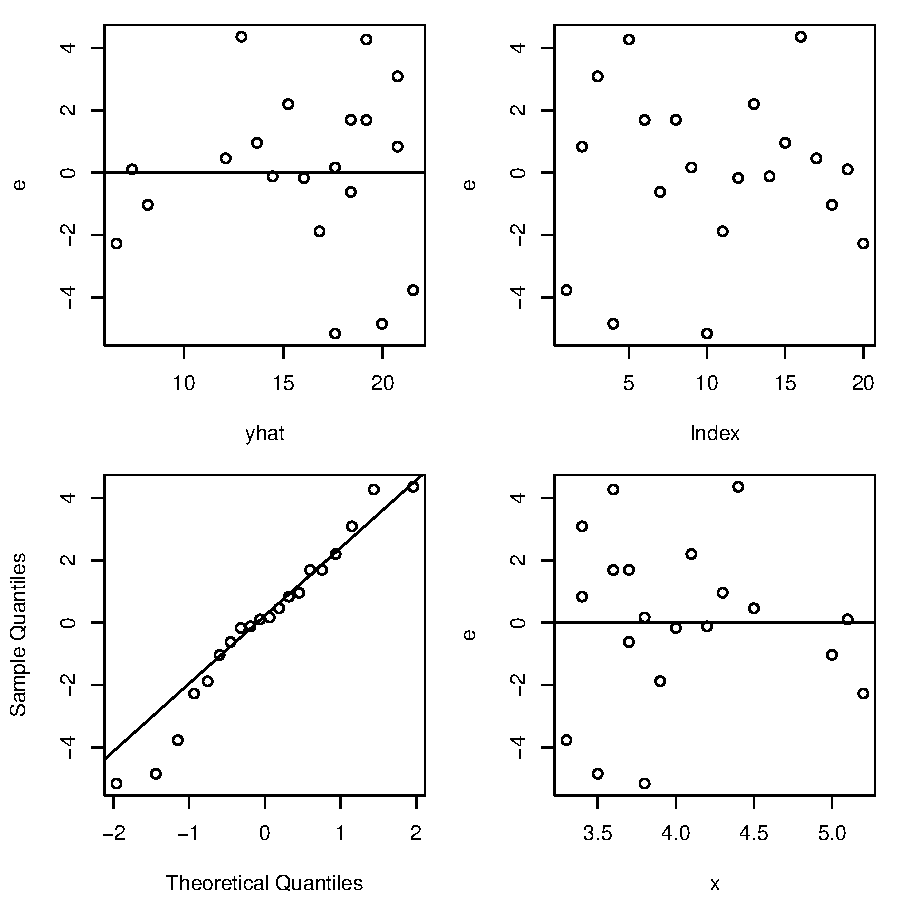
\includegraphics{11-4_diagnostic}}
\end{center}
\caption{Diagnostic plots for the data in Example~11-4 of Ott \& Longnecker.}
\label{fig:11-4_diagnostic}
\end{figure}

\begin{example}[11-10 in Ott \& Longnecker]
The data and R code for this example are posted on the course website.  The four diagnostic plots are displayed in Figure~\ref{fig:11-10_diagnostic}.  In this case, we see a clear pattern in the first of the four plots, indicating that there is some structure that was not accounted for by the linear part of the model.  A natural strategy would be to include an extra variable, e.g., $x^2$, to capture that structure.  You saw this in lab and the R code on the website also shows this.  
\end{example}

\begin{figure}
\begin{center}
\scalebox{0.75}{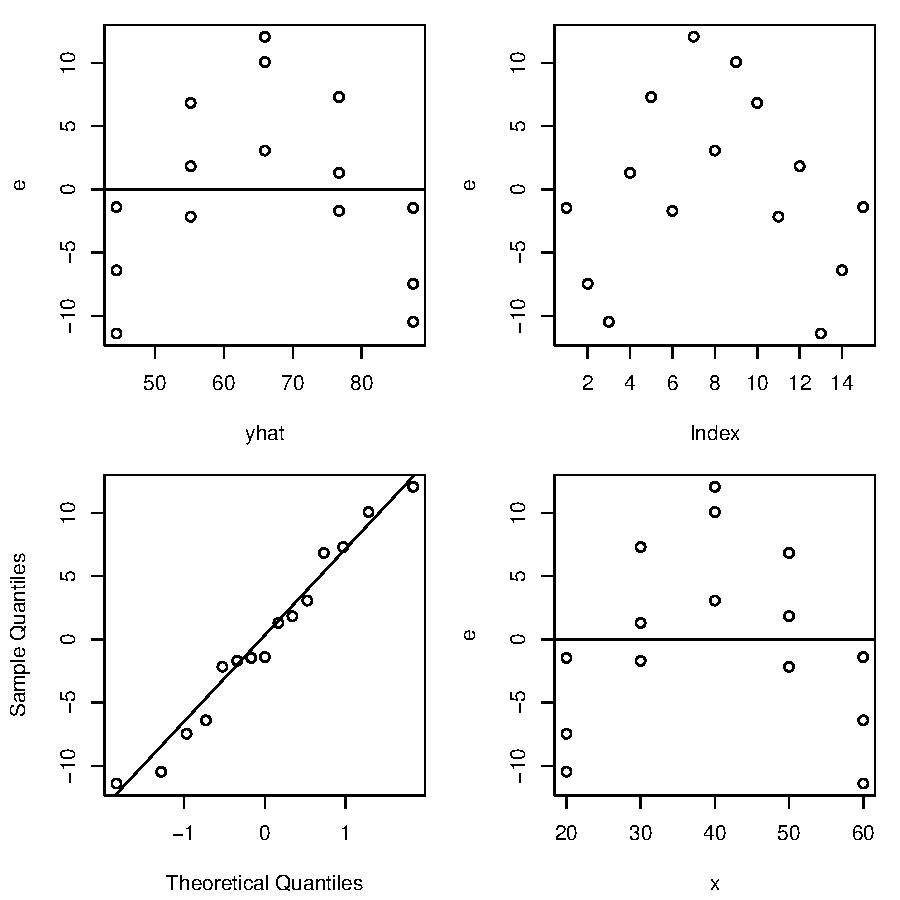
\includegraphics{11-10_diagnostic}}
\end{center}
\caption{Diagnostic plots for the data in Example~11-10 of Ott \& Longnecker.}
\label{fig:11-10_diagnostic}
\end{figure}

You've now seen two examples where we've looked at the diagnostic plots and tried to make a judgment about whether the assumptions of the linear model appear to be reasonable.  Two examples is definitely not enough to make you an expert, so don't worry if you're still unsure about how to deal with this.  One thing that can help is to {\em simulate} some fake data where you know the assumption is satisfied, and then see what the corresponding plots look like.  Doing this multiple times can help to calibrate your expectations for real examples.\footnote{We did this in class with the QQ plot, and we found that, in three separate data sets, twice the points were close to the diagonal line and once they weren't.  How far the points were from the line in the latter case helps to inform us about how far away the points need to be in a real data example for us have serious concerns about the normality assumption.}  Aside from telling you what plots to look at and showing you how to calibrate your expectations about what these plots ought to look like if the assumptions are satisfied, there's not much else I can say here.  There will be certain instances in ST512 where there will be some feature I expect for you to see in a diagnostic plot (e.g., on an exam), and not spotting that feature will make you ``wrong,'' but in real life there is no right/wrong with these plots.  Your PhD committee members or a reviewer of your research paper might question a choice you made, but they aren't right/wrong either, they just have a different opinion.  So what matters is how you justify the choices you make, and that's what these plots are for.  For example, if your advisor asks you why a normality assumption is reasonable, you can show her the plot and say something like this: ``as the QQ plot on page~7 shows, the quantiles of the residuals are within an acceptable range of the quantiles of the normal distribution, so there is no serious reason to doubt the normality assumption.''  

\begin{example}[BUPA]
One last example, which is not from the textbook, investigates the relationship between two blood measurements that relate to liver disorder.\footnote{See \url{http://archive.ics.uci.edu/ml/datasets/Liver+Disorders}}  The two variables we consider here are the 3rd and the 5th, namely, {\tt sgpt} ({\em alanine aminotransferase}) and {\tt gammagt} ({\em gamma-glutamyl transpeptidase}).  Here I am taking the response variable, $y$, to be {\tt sgpt} and the explanatory variable, $x$, to be the logarithm of {\tt gammagt}.  (I don't know if there's any scientific reason for looking at this particular pair of variables or in this order.)  The top row of Figure~\ref{fig:bupa} shows the scatter plot of $y$ vs $x$ along with the fitted regression line.  We can immediately see some potential trouble because the cloud of points fans out on the right.  The effect of this fanning is seen in the residual plot next to it, there's a very obvious megaphone shape, suggesting the constant variance assumption is questionable.  A strategy that often works to correct for non-constant variance is to make a (cleverly-chosen) transformation.  In this case, a transformation that seems to work well\footnote{There is some ``advanced'' statistical method that suggests this logarithmic transformation, but we won't discuss this in ST512.  If you're interested, the method is called the {\em Box--Cox power transformation} and a summary of the main idea is here: \url{https://en.wikipedia.org/wiki/Power_transform}} is to replace $y$ with $\log y$.  After making this change, fitting the regression model with the new/transformed response, we get generate the same plots as before, shown in the bottom row of Figure~\ref{fig:bupa}.  There's a lot less fanning the left-most panel and, as a result, we no longer see the megaphone shape in the right-most panel.  Therefore, the constant variance assumption would be satisfied for a model that relates $\log y$ to $x$.  Such a model would still allow researchers to understand the relationship between the original variables {\tt sgpt} and {\tt gammagt}, but there's some math needed to see this precisely:
\[ \log {\tt sgpt} \approx \beta_0 + \beta_1 \log ({\tt gammagt}) \iff {\tt sgpt} \approx e^{\beta_0} ({\tt gammagt})^{\beta_1}. \]
\end{example}

\begin{figure}
\begin{center}
\scalebox{0.75}{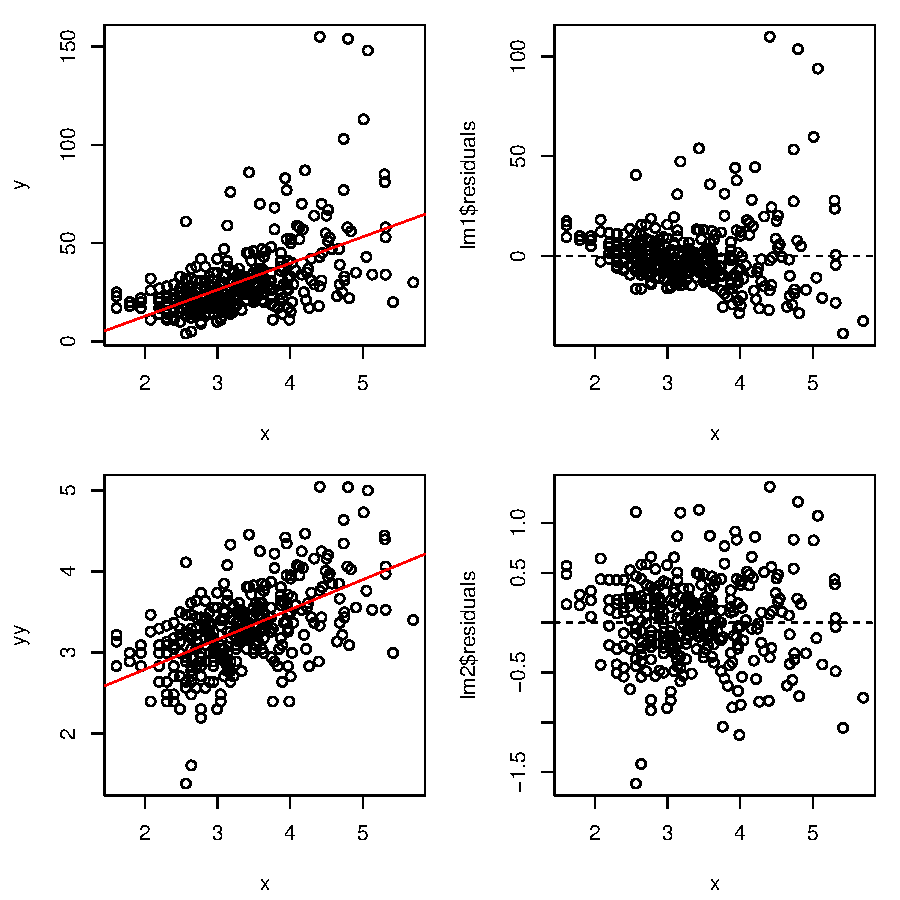
\includegraphics{bupa}}
\end{center}
\caption{Plots for the BUPA data example.}
\label{fig:bupa}
\end{figure}

%A few comments about p-hacking, etc...

(01/29/2019) The last topic for this section is {\em correlation}.  This is a measure of the strength and direction of a {\bf linear} relationship between two variables.  We can rely on the software to do the necessary computations for us, but it may help to keep in mind that correlation is just a number calculated from the $(x,y)$ data pairs:
\[ r = \frac{\sum_{i=1}^n (x_i - \bar x)(y_i - \bar y)}{\sqrt{ \sum_{i=1}^n (x_i - \bar x)^2 \cdot \sum_{i=1}^n (y_i - \bar y)^2}}. \]
We will look at the {\em magnitude} and {\em sign} of the correlation coefficient, $r$.  
\begin{itemize}
\item $-1 \leq r \leq 1$, and larger magnitude indicates stronger relationship; 
\vspace{-2mm}
\item The sign, positive or negative, describes the direction of the linear relationship.
\end{itemize}
Therefore, $r \approx 1$ means a strong positive linear relationship; $r \approx -1$ means a strong negative linear relationship; and $r \approx 0$ means basically no linear relationship.  Figure~11.21 in Ott \& Longnecker shows illustrations of a bunch of different cases.  We won't rely too much on correlation in ST512, but it's an important concept to know.  From time to time, I may talk about a pair of variables being {\em highly correlated} which means their correlation is close to $\pm 1$.  

I also need to emphasize that correlation should only be used for measuring the strength/direction of {\em linear relationships}.  In fact, it is possible for a pair of variables to be strongly related (but in a non-linear way) and for the correlation to be zero or near zero.  So, just blindly looking at $r \approx 0$ might lead you to (incorrectly) conclude that the variables aren't related when, in fact, they are strongly related, just in a non-linear way.  





\section{Multiple linear regression}

\subsection*{01/29/2019}

So far, we have been focusing on situations in which there are only two variables in question, a response variable $y$ and an explanatory variable $x$.  For these situations, we might be able to use simple linear regression to capture the relationship between the two, e.g., for predicting the value of $y$ and a value of $x$.  But in any interesting real problem, there are likely to be more than two relevant variables.  For example, with the beer consumption and blood alcohol content data from a while back, we only had number of beers consumed ($x$) and blood alcohol level ($y$).  But it's likely that the individual's size, gender, age, etc., would also affect how beer consumption is converted to alcohol level in the blood, so if we had that information available to us, then we'd naturally want to make use of it.  We are familiar with weather predictions on the news, and the weatherman will often talk about a ``computer model'' that describes the weather patterns and produces the predictions; this is just a more complicated version of what we're going to talk about, i.e., incorporating information in several explanatory variables to help in understanding/predicting the response.  

Imagine a spreadsheet that has several columns: one for the response, $y$, and one for each of the variables $x_1, x_2, \ldots, x_k$.  We'll see concrete versions of these spreadsheets in our examples.  The natural generalization of that simple linear regression model from before is 
\[ y_i = \beta_0 + \beta_1 x_{i,1} + \beta_2 x_{i,2} + \cdots + \beta_k x_{i,k} + \eps_i, \quad i=1,\ldots,n, \]
where $x_{i,j}$ denotes the value of variable $j$ for individual $i$, $\beta_0$ is the intercept, $\beta_j$ is the slope corresponding to variable $x_j$, and the errors---$\eps_1,\eps_2,\ldots,\eps_n$---are assumed to be independent and identically distributed, $\nm(0,\sigma_\eps^2)$, just like before.  

Following the same path as in the simple linear regression setting, the first task is to estimate the unknown parameters.  Here we have potentially a lot more parameters than before, but we will continue to rely on the software to do the computations.  That is, we can read off the estimates $\hat\beta_j$ of $\beta_j$ from the SAS/R output; similarly, the estimate $\hat\sigma_\eps^2$ of $\sigma_\eps^2$ is just the mean square error (MSE).  There is a fitted regression line 
\[ \hat y(\tilde x_1, \ldots, \tilde x_k) = \hat\beta_0 + \hat\beta_1 \tilde x_1 + \cdots + \hat\beta_k \tilde x_k, \]
which we can get for any tuple $(\tilde x_1, \ldots, \tilde x_k)$.  Like before, the fitted value at the $x$ values for individual $i$ are denoted as $\hat y_i$.  Unfortunately, we can rarely draw a plot of this fitted model because now there is no ``line.''  In the case with only two explanatory variables, $x_1$ and $x_2$, the object $\hat y(\cdot)$ is a plane in three-space.  In the general case, $\hat y(\cdot)$ is a {\em hyperplane} in $(k+1)$-space and it can't be visualized.  So we have to rely on other tools for visualization.  

Note also that the interpretation of $\hat\beta_j$ is as the change in the mean response corresponding to a unit change in variable $x_j$, holding everything else fixed.  

Since the assumptions about the errors are the same as before, you might expect that the diagnostics plots we use to check those assumptions are the same, and you'd be correct.  We still rely on the residuals vs.~fitted, QQ plot of residuals, and residuals vs.~individual $x_j$'s to check our assumptions.  The residual vs.~fitted plays a much more important role now than it did before, because this is the only plot we have for checking if the linearity assumption seems reasonable---remember, we can't draw a scatterplot to visualize the $y \times (x_1,\ldots,x_k)$ relationship anymore because the dimensions are too high.  Discernible patters in this residuals vs.~fitted plot would indicate that a linear relationship between $y$ and $(x_1,\ldots,x_k)$ might not be appropriate.  

More on hypothesis tests, etc., next time...


\subsection*{01/31/2019}

Following the fit of the model and an assessment of the underlying assumptions, we're ready to start asking (scientific and statistical) questions about the relationship between the response $y$ and the available predictor variables $x_1,\ldots,x_k$.  There's a first basic question that should always be asked, that is, {\em is $y$ related to any of the $x$'s?}  If the answer to this question is NO, then there is no reason to proceed with consideration of the model that is based on there being a relationship.  For example, if there's no relationship, then it wouldn't make sense to use the $x$ variables to predict the $y$ value.  So, before we do anything, we should first establish the existence of a relationship to be explored further.  

Just like in simple linear regression (and in the examples before we started regression), we want to encode this scientific question into statistical terms.  In this case, the question about there being any relationship between $y$ and $x_1,\ldots,x_k$ corresponds to a hypothesis
\[ H_0: \beta_1 = \beta_2 = \cdots = \beta_k = 0, \]
i.e., that all the slope coefficients are simultaneously equal to 0.  The point is that, if all the $\beta$'s are 0, then changing any of the $x$ variables won't change $y$, hence no relationship.  This is a very weak hypothesis so you should almost always expect that it will be rejected, the point being that you probably wouldn't have collected these variables in the first place if there really was no relationship.  So the point of this test is basically to determine if the data is of sufficient quality (e.g., not too much noise) to be able to assess even a most basic question.  

Our test of this hypothesis relies on an importance concept, namely, the {\em partitioning of the sum of squares}.  This is fundamental to most of the theory underlying the methods used in ST512 and, perhaps surprisingly, is just an application of the Pythagorean Theorem from high-school geometry.  This is expressed mathematically as follows:
\[ \underbrace{\sum_{i=1}^n (y_i - \bar y)^2}_{\text{SS(Total)}} = \underbrace{\sum_{i=1}^n (y_i - \hat y_i)^2}_{\text{SS(Error)}} + \underbrace{\sum_{i=1}^n (\hat y_i - \bar y)^2}_{\text{SS(Model)}}, \]
where $\bar y$ is the sample mean of the response and $\hat y_i$ is the fitted value.  The abbreviations underneath are ``SS'' for Sum of Squares, so we have a decomposition of the total sum of squares into a sum of squares corresponding to error (this is the sum of the squared residuals, $e_i^2$) and a sum of squares corresponding to the regression model.  Notice that the SS(Total) is a feature of the data and cannot be changed by any analysis we choose to perform.  But SS(Error) and SS(Model) can be changed by our choice of what model to fit.  A model that is ``good'' is one that has small errors and, in such cases, the majority of SS(Total) would be made up of SS(Model).  The {\em coefficient of determination}, a basic measure of model fit, is based on this:
\[ R^2 = \frac{\text{SS(Model)}}{\text{SS(Total)}} = \text{proportion of variation in $y$ explained by model}. \]
If $R^2$ is relatively large, then SS(Model) is relatively close to SS(Total), which means that SS(Error) is relatively small; therefore, relatively large $R^2$ is an indication of good model fit.  I'll have to add some extra qualifications to this statement later...

Back to the hypothesis test.  Intuitively, if SS(Model) is relatively large or, equivalently, if SS(Error) is relatively small, then there must be something good about including the $x$ variables in the model and, hence, there must be some relationship between $y$ and the $x$ variables.  The specific measure of the relative magnitudes of SS(Model) and SS(Error) used in this context is the following F statistic:
\[ F = \frac{\text{MS(Model)}}{\text{MS(Error)}} = \frac{\text{SS(Model)} / \text{df(Model)}}{\text{SS(Error)} / \text{df(Error)}}. \]
There's some adjustment factor in terms of the degrees of freedom, but this is basically just the ratio of SS(Model) to SS(Error) and, therefore, is basically just $R^2$.  We will reject $H_0$ if $R^2$ is too close to 1 or, equivalently, if $F$ is too large.  The specific scale on which $F$ is to be assessed is determined by a F-distribution,\footnote{There are tables of F-distribution critical values in Ott \& Longnecker.} a close relative to the t-distribution.  For us, it's fine to rely on the p-value calculation from R/SAS.  The point is that p-value will be small when $F$ is large.  I call this the {\em overall F-test}.  

\begin{example}[12-6 in Ott \& Longnecker]
SAS code on the course website.  Look for the SS and MS in the Analysis of Variance table; you can see the partitioning of sum of squares and also the $F$ statistic and p-value. 
\end{example}

In some sense, we haven't done anything yet.  This overall F-test answers only the first basic question: is there anything interesting going on between $y$ and these $x$'s.  Usually we already know something should be going on, otherwise we wouldn't have done the study, so this is test is effectively just a check that the data meets some minimal quality standards.  What comes after rejecting the overall F-test is a series of more interesting follow-up questions.  

One type of follow-up question is if $y$ is related to a specific $x$ variable.  For example, we can address the question {\em is $y$ related to $x_1$?} by testing a hypothesis $H_0: \beta_1 = 0$.  This can be done exactly like we did in the simple linear regression case, using the $t$-statistic and p-value that shows up in the ``Parameter Estimates'' table from the software.  

There are intermediate cases between tests about all variables and tests about single variables.  In particular, we can ask about any subset of the variables.  This generalizes what we did above with the individual t-test.  The way we carry out these tests is to effectively fit two different models and compare their quality of fit.  More next time...


\subsection*{02/05/2019}

We will encounter cases where there are a subset of the variables whose importance is in question.  Suppose that we have $k$ predictor variables: $x_1,x_2,\ldots,x_k$.  Next, suppose there is a subset of $g$ many variables, say, $x_1,\ldots,x_g$, with $g < k$ that are assumed to be important, and the remaining variables, $x_{g+1},\ldots,x_k$, are of questionable importance.  That is, we are considering the question {\em are $x_{g+1},\ldots,x_k$ related to $y$?}  If the $\beta$ coefficients attached to these questionable variables are all equal to 0, then changing these variables won't impact $y$, hence we'd say that they're not important.  So the version of this question in hypothesis form is like this
\[ H_0: \beta_{g+1} = \cdots = \beta_k = 0. \]
I'll refer to the test we will carry out here as the {\em partial F-test} because it's like the overall F-test but only involves a subset of the predictor variables.  It proceeds by considering two different models, a {\em full model} and a {\em reduced model}.  The full model includes all the variables while the reduced model only includes those variables {\em not} in the questionable set, that is, variables $x_1,\ldots,x_g$.  In the example that follows, the response variable is {\tt catch} and there are $k=4$ variables: {\tt residence}, {\tt size}, {\tt access}, and {\tt structure} and it is assumed that {\tt residence} and {\tt size} are important, but {\tt access} and {\tt structure} might not be.  So the full and reduced models are 
{\small
\begin{verbatim}
      Full: model catch = residence size access structure;
   Reduced: model catch = residence size; 
\end{verbatim}
}
Both of these model fits have a corresponding partitioning of the sum of squares, and these can be easily obtained from the model fits in SAS or R.  From these, we can form the test statistic
\[ F = \frac{\{\text{SS(Model, full)} - \text{SS(Model, reduced)}\}/(k-g)}{\text{MS(Error, full)}}. \]
If this $F$ value is large, then that means $\text{SS(Model, full)}$ is quite a bit larger than $\text{SS(Model, reduced)}$ and, therefore, by the Pythagorean theorem stuff before, it must be that $\text{SS(Error, reduced)}$ is quite a bit larger than $\text{SS(Error, full)}$.  And if the reduced model has a lot more error than the full model, then it must be that the omitted variables in the reduced model are important, which is evidence against $H_0$.  Similarly, if $F$ is small, then it must be that the error sums of squares for the full and reduced models are about the same, hence those omitted variables are not important, which is evidence for $H_0$.  So, we reject $H_0$ if and only if $F$ is sufficiently large.  The easiest way to tell if $F$ is large or not is to convert it to a p-value.  There are a number of ways to do this, one is to ask SAS to carry out the specific partial F test.  This requires adding a line to the code, with keyword {\tt test}.  This will give you a special table with the numerical values of the numerator and denominator in the expression for $F$ above, along with the $F$ ratio and the corresponding p-value.  

\begin{example}[12-17 in Ott \& Longnecker]
SAS code on the course website.  Check that you get the same value for $F$ by reading the sums of squares from the individual Analysis of Variance tables and plugging into the above formula as you do in the table based on the {\tt test} request.  The results from the partial F test in R are given below; the p-value is very small so we would be inclined to reject $H_0$, and conclude that {\tt access} and {\tt structure} are important variables. 
{\small 
\begin{verbatim}
   Analysis of Variance Table

   Model 1: catch ~ residence + size
   Model 2: catch ~ residence + size + access + structure
     Res.Df     RSS Df Sum of Sq      F    Pr(>F)    
   1     16 23.4248                                  
   2     14  2.2749  2     21.15 65.079 8.147e-08 ***
   ---
   Signif. codes:  0 ‘***’ 0.001 ‘**’ 0.01 ‘*’ 0.05 ‘.’ 0.1 ‘ ’ 1
\end{verbatim}
}
\end{example}

Changing gears a bit, I want to talk about the different kinds of predictor variables we might encounter.  What we're most familiar with are {\em numerical variables}, e.g., number of beers consumed, blood alcohol content, etc.  But we might also encounter {\em categorical variables}, e.g., {\tt size} taking values ``small,'' ``medium,'' and ``large,'' or {\tt dose} taking values ``low'' and ``high,'' or {\tt drug} taking values ``A,'' ``B,'' and ``C.''  The challenge with categorical variables is that we can't put these into a mathematical model like regression because it doesn't make sense to multiply ``medium'' by 7, or to add 3.3 to it.  We can only do these mathematical operations on numbers, but categorical variables don't have numerical values.  An idea would be to convert ``low'' and ``high'' to, say, values 1 and 2, but it's not so simple.  For example, does it make sense to say that ``high'' is twice as much as ``low''?  Maybe not.  And the values 1 and 2 were totally arbitrary, one could have alternatively said ``low'' was 17 and ``high'' was 92.  Care is needed to convert categorical variables into numerical variables that we can include in our regression models.  

The specific approach we use here is to create {\em dummy variables}.  If a categorical variable has $L$ levels, then it will require the construction of $L-1$ dummy variables.  For example, consider variable {\tt drug} with $L=3$ levels, labeled A, B, and C.  One way\footnote{There are lots of different ways to do the coding of a categorical variable into a set of dummy variables, all equally good.  The only difference is in the interpretation of the parameter estimates, which comes later.} to express this in terms of dummy variables, say, $x_1$ and $x_2$ is as follows:
\[ x_1 = \begin{cases} 1 & \text{if {\tt drug} is A} \\ 0 & \text{otherwise} \end{cases} \quad \text{and} \quad x_2 = \begin{cases} 1 & \text{if {\tt drug} is B} \\ 0 & \text{otherwise}. \end{cases} \]
That is, level A corresponds to $(x_1,x_2) = (1,0)$, level B corresponds to $(x_1,x_2)=(0,1)$, and level C corresponds to $(x_1,x_2) = (0,0)$.  There will be some more convenient ways to deal with categorical variables, which we'll see a bit later, but for now we have to do the dummy variable construction.  The SAS code for Example 12-21 in Ott \& Longnecker on the website shows how to create a dummy variable in the data step.  

Categorical variables is another situation where variables are naturally grouped and a partial F test may be required.  For example, we might want to include variable {\tt drug} in a multiple linear regression model using the two dummy variables as above.  If we wanted then to test if the {\tt drug} variable is important, we need to consider the pair $(x_1,x_2)$ together; the individual dummy variables themselves are meaningless, only together do they have an interpretation.  So, if the model is 
\[ y = \beta_0 + \beta_1 x_1 + \beta_2 x_2 + \cdots + \eps, \]
and we want to know if {\tt drug} is an important variable, we would consider a null hypothesis $H_0: \beta_1 = \beta_2 = 0$, for which we would employ a partial F test as described above.  

More on the analysis of models involving categorical predictors next time...



\subsection*{02/07/2019}

Last time we discussed categorical predictor variables and how they're coded in terms of a set of dummy variables.  We'll get lots of experience working with the categorical variables when we finish with the section on multiple linear regression, but for now I want to focus on an interesting special case of regression, one where we have a single numerical predictor variable, $x_1$, and a categorical predictor with two levels that can, therefore, be described by a single dummy variable, $x_2$, which takes values 0 or 1 only.  The example discussed in class is one where the numerical predictor variable is a dose level of a drug while the categorical variable is the type of drug being administered.  The model to be considered is 
\[ y = \beta_0 + \beta_1 x_1 + \beta_2 x_2 + \eps. \]
All the usual assumptions are in play here.  We are primarily interested in the way that the categorical/dummy variable $x_2$ impacts the relationship between the response $y$ and the numerical variable $x_1$.  

Towards this, let's consider what happens for the two cases of $x_2$ separately.
\begin{itemize}
\item {\em Assume $x_2=0$}.  If $x_2=0$, then $\beta_2$ doesn't enter into the equation at all, so the model becomes 
\[ y = \beta_0 + \beta_1 x_1 + \eps, \]
which is exactly like our simple linear regression discussed before.  
\item {\em Assume $x_2=1$}.  If $x_2=1$, then $\beta_2$ does enter into the equation, and the model becomes 
\[ y = (\beta_0 + \beta_2) + \beta_1 x_1 + \eps. \]
That is, $\beta_2$ shows up but {\em not} like a slope as we're used to.  In this case, it plays the role of an intercept adjustment. 
\end{itemize}
In this {\em additive} model (to be compared to the {\em interaction} model below), the impact of the categorical predictor variable on the $(x_1,y)$ relationship is a shift or change-in-intercept only.  That is, the level of $x_2$ doesn't impact the rate at which $y$ changes with $x_1$.  In the context of the example, patients' response to a change in the dose level is the same for both types of drugs.  That's at least what the additive model assumes---the data may not be consistent with that assumption, however.

As hinted at above, there is another model involving these two variables that we might consider.  If we multiply the two predictor variables, then we call the product $x_1x_2$ the {\em interaction}, and we can include this interaction term in the model as follows:
\[ y = \beta_0 + \beta_1 x_1 + \beta_2 x_2 + \beta_3 x_1x_2 + \eps. \]
To understand the role of the interaction term, let's do the same breakdown as before.
\begin{itemize}
\item {\em Assume $x_2=0$}.  If $x_2=0$, then neither $\beta_2$ nor $\beta_3$ enters the model, which is
\[ y = \beta_0 + \beta_1 x_1 + \eps, \]
which again is exactly like our simple linear regression discussed before.  
\item {\em Assume $x_2=1$}.  If $x_2=1$, then $\beta_2$ and $\beta_3$ enter into the equation, and we get 
\[ y = (\beta_0 + \beta_2) + (\beta_1 + \beta_3) x_1 + \eps. \]
That is, $\beta_2$ shows up as a change in intercept and $\beta$ as a change in slope.  In this more general model, the categorical predictor variable does impact the rate (and possibly even the direction) in which $y$ changes with $x_1$.  
\end{itemize}
In terms of our example, the interaction model says that patients' response to a change in the dose level depends on which drug they are taking.  

There's an important scientific question that can now be easily addressed using this model setup.  The question is: {\em does the type of drug affect the way in which patients respond to changes in the dose level?}  To answer this, it is clear that we want to test 
\[ H_0: \beta_3 = 0, \]
and we already know how to handle this, it's just an individual t-test on the coefficient attached to the interaction term.  

\begin{example}[12-21 in Ott \& Longnecker]
SAS code on the website.
\end{example}

The last bit of material I want to cover for the section on multiple linear regression is {\em model building and assessment}.  There can (and maybe should) be an entire course devoted to this single topic because it's easily the most difficult part of statistical analysis and there are so many things that could be said.  The point, as I mentioned a while back in various contexts, is that there is generally no ``right'' model and ``wrong'' model, so you have to make a judgment call.  All I can do here in ST512 is to present some of the tools that can be used to help you make that judgment.  If it were a real context, then I could look at all the available information and formulate my own judgment/recommendation to the scientist, but there's more that goes into such a formulation than can be covered in a single ST512 lecture and, ultimately, even my own ``expert'' recommendation would come with no guarantees of being correct, since ``correct'' isn't even defined in this context.  Anyway, my goal is to focus here on basics.  

To set the scene, we have a response variable that we're interested in, and a bunch of candidate predictor variables, say, $x_1,\ldots,x_k$.  Note that some of these predictor variables could be transformations (e.g., quadratic or interaction terms) involving some of the other variables, that's fine.  Once the set of variables is in place, the hard work begins.  The key question is: {\em which variables to include in the model?}  One possibility is the full model 
\[ y = \beta_0 + \beta_1 x_1 + \beta_2 x_2 + \cdots + \beta_k x_k + \eps, \]  
the model with all the variables.  But there are {\em lots} of possible reduced models that could be considered, often too many to actually consider all of them.\footnote{Later I'll have a few things to say about the dangers in searching over all or many candidate models...}  Here I believe it's best to rely on expert knowledge about the context, not just on statistical methods.  If there are variables you expect to be important, then put them in.  This expert knowledge likely won't be enough to fully determine a sound model, but it simplifies the search tremendously.  I'll focus here on only the {\em statistical} considerations, because that's all we can do here, but please keep in mind that {\em scientific} considerations are more important.  

In terms of statistical considerations, an obvious first question is {\em why not just pick the model that fits the best?}  Good idea, but there's one problem: the full model always fits the best.  As is true in any kind of optimization problem, you can always do better with more flexibility.  The full model, in our case, has the most flexibility and, therefore, if we want to optimize fit, then we would always pick the full model.  But this is not satisfactory for several reasons.  First, some of the variables we start with surely are not important. As an extreme example, plants in a study might be given an ID number and, surely, that ID number wouldn't be relevant to the plant's response to a fertilizer treatment; but including that ID variable definitely will not make the model fit worse.  Second, having more variables in the model makes it more difficult to estimate the parameters in that model accurately so, even though the model might ``fit well,'' we may not be able to answer the relevant scientific questions definitively because, say, the test about $\beta_1$ has too low of power.  So fit alone is not a useful metric for determining a sound model.  

There are various ways to get around this, differing in their technical details, but they all share a common motivation.  That is, the revised goal is to balance {\em quality of fit} with {\em complexity of the model} in some suitable way.  This is an application of {\em Occam's Razor},\footnote{\url{https://en.wikipedia.org/wiki/Occam\%27s_razor}} the law of parsimony.  That is, try to find the simplest model that also has good fit.  One strategy is to work with a so-called {\em adjusted $R^2$}.  Recall, the original $R^2$ is a measure of fit alone, so it is always the case that the full model has the largest $R^2$ value among the candidate models.  But this formula can be adjusted to take into account the complexity (number of variables) included in model.  The book gives a formula for the adjusted $R^2$ on page~719 but that's not important for us here.  What matters is that the adjusted $R^2$ is not necessarily increasing when a variable is added, i.e., that adding a variable of little importance might make the adjusted $R^2$ go down.  So if we choose a model that makes the adjusted $R^2$ as large (or nearly as large) as possible, then in some sense we've accomplished the balance between fit and complexity.  Other kinds of scores besides adjusted $R^2$ are possible too, e.g., the Akaike Information Criterion (AIC) and the Bayesian Information Criterion (BIC), also defined in the book.  The thing to keep in mind is that you're looking for adjusted $R^2$ to be large, but you look for small values of AIC and BIC.  

\begin{example}[13-3 in Ott \& Longnecker]
SAS code on the website.
\end{example}

%{\color{red} There's some (technical) points I may not have time to make during the class but I'll add them here later.}


\subsection*{02/19/2019}

There's a few points I'd like to make here to wrap up the presentation about multiple linear regression.  Both are technical in nature but important enough that I feel obligated to discuss even though this is a non-technical course.  

The first is about {\em multicollinearity}, i.e., when there is strong correlation/dependence between predictor variables.  Remember that strong correlation between predictor variables and the response variable is desirable, because it suggests the predictors are informative, but strong correlation between the predictors themselves can cause problems.  The reason for the problems is technical, so I won't get into those details,\footnote{Virtually all of the calculations SAS is doing behind the scenes are linear algebra operations, e.g., matrix/vector multiplication, matrix inversion, etc.  When variables are highly correlated, it can happen that the particular matrix SAS needs to invert is almost non-invertible, so the inverse operation is unstable.  Also, standard errors of the $\beta$ estimates are related to this inverse matrix; just like dividing by a very small number makes the ratio big, if you try to invert a ``very small'' matrix, then you get large standard errors.} but I can say that the problems caused by multicollinearity usually manifest in the form of very large standard errors on the $\beta$ parameter estimates (which might cause individual t-tests to fail to reject) and some inconsistent conclusions, e.g., where the overall F-test rejects but none of the individual t-tests do.  If you see such things in your output, then this might be a sign of multicollinearity so you should investigate the correlation between predictors more carefully and take some action to remedy it.  The simplest action is to remove one of a pair of predictor variables that are highly correlated, but this may require some scientific judgment; there are other more sophisticated approaches (e.g., principle component analysis) that can be used to remove redundant variables, but this is beyond what we cover in ST512.  

The second is about {\em selection bias}.  The theory that all the tests, confidence intervals, etc., presented in ST512 are based assumes that the model being fit is pre-determined, in particular, that the data itself {\em doesn't} inform our choice of model, or hypotheses to test, etc.  However, our model-building strategies are all based on the idea that we fit one model, check if it seems good in some sense based on the SAS output, and then revise if necessary.  So, at the end of this process, the data informed our choice of the model being fit and, since some predictor variables likely have been omitted, it informs what hypotheses we choose to test.  For example, if predictor variable $x_1$ remains in my model at the end of the building steps, then I might want to report a confidence interval for the corresponding $\beta_1$; but I wouldn't report such a confidence interval if $x_1$ had been excluded from the model.  This is a concern because it affects our ability to justify the conclusions we make based on the final model fit.  Here's a simple example.

\begin{example}
If I have a single data observation, $Z_1$, which is assumed to be $\nm(\mu_1,1)$ for some unknown mean $\mu_1$.  In ST511 you discuss how to test $H_0: \mu_1 = 0$.  That is, if $|Z_1| > 1.96$, then you reject $H_0$.  Why is this testing procedure justified?  Because it guarantees that you make a Type~I error only 5\% of the time.  Now consider a different scenario, where $Z_j$ is $\nm(\mu_j, 1)$, for $j=1,2,\ldots,10$, say.  The point is that there's different means to test.  Suppose I choose which mean to test by finding the ``most extreme'' data point.  That is, let $j^\star$ be such that $|Z_{j^\star}| = \max_j |Z_j|$,corresponding to the ``most extreme'' observation, and consider testing $H_0: \mu_{j^\star}=0$.  At this point, the problem looks similar to the one above, so it is tempting to adopt the following testing procedure: reject $H_0$ if $|Z_{j^\star}| > 1.96$.  The question is: {\em does this testing procedure control Type~I error at 5\%?}  No it does not, that this is the selection bias.  Here's an R code simulation to check my claim:
{\small
\begin{verbatim}
> p <- 0
> for(i in 1:5000) p <- p + (max(abs(rnorm(10))) > 1.96) / 5000
> print(p)
[1] 0.399
\end{verbatim}
}
\noindent In this simulation, all of the $\mu_j$'s are 0 so, in particular, $\mu_{j^\star}$ is 0, and hence the null hypothesis is true.  The quantity {\tt p} reported above represents the proportion (out of 5000 tests) that a Type~I error was made, and we see that it's about 40\%.  So that testing rule that was theoretically justified with just a single test to consider because faulty if applied after data was used to select the hypothesis to be tested.  
\end{example}

This phenomenon can arise in more complicated/realistic problems too, in perhaps more severe forms.  The following, which is still illustrative in nature, will hopefully reveal the potential risk.

\begin{example}
Consider a regression setting with, say, 10 predictor variables.  We discussed the use of AIC to select a good model; in what follows, nothing is specific to AIC, it's just that AIC-based selection is relatively easy in R.  Here's the experiment: first I'm going to simulated data such that the null hypothesis, $H_0: \beta_1 = \cdots = \beta_{10} = 0$, is true; then I'm going to pick the subset of those 10 predictor variables that is best according to the AIC criterion; finally, I'm going to carry out the overall F-test {\em on the selected set of variables} and return the p-value.  Since the null hypothesis is true, the theory for the overall F-test suggests that the p-values should be uniformly distributed, so we only get p-value less than 0.05 in 5\% of the cases.  Figure~\ref{fig:aic.ftest} shows the distribution of these p-values and we see that far more than 5\% of the p-values are less than 0.05, hence lots of Type~I errors.  
\end{example}

\begin{figure}
\begin{center}
\scalebox{0.75}{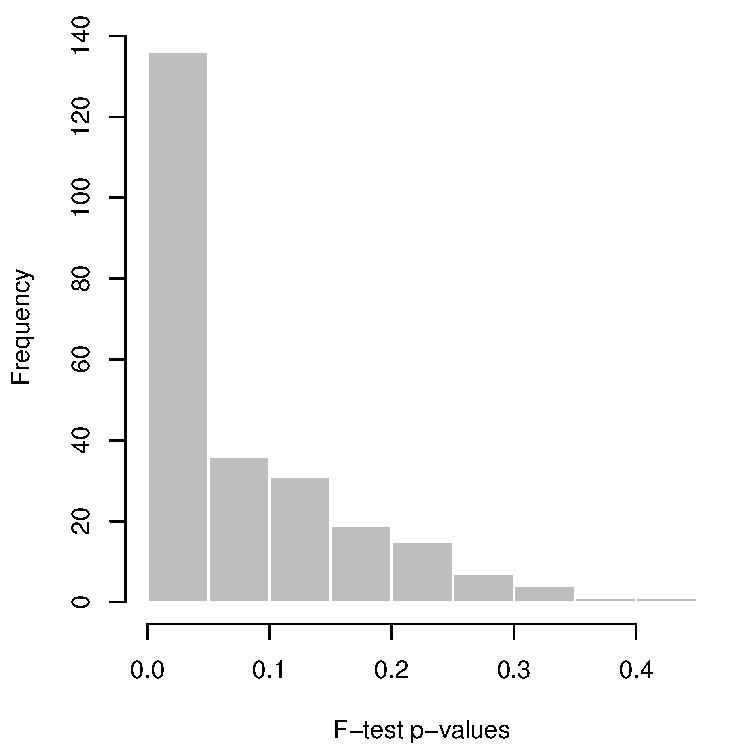
\includegraphics{aic_ftest_hist}}
\end{center}
\caption{Histogram of p-values for the overall F-test under the null hypothesis applied {\em after} a model selection step.}
\label{fig:aic.ftest}
\end{figure}

To be clear, this is not a sign that the theory is faulty: the problematic tests in the examples above are the result of procedures being applied in situations where they were not intended to be applied.  This is why an understanding of the theory is important---and why ST511--512 is not a sufficient introduction to applied statistics.  Anyway, statisticians are in the process of trying to understand the selection bias and developing new methods to overcome it, but this is a very challenging problem.\footnote{I wrote a paper (\url{https://arxiv.org/abs/1712.02379}) about some of these issues, but mine was more along the lines of identifying a particular problem/bias, not about fixing it, unfortunately.}  All I can say here is that the data-driven model-building techniques discussed in class before (e.g., ranking candidate models based on AIC) is a valuable tool, but be aware of the risks in carrying out inferences (and predictions) about parameters in the selected model using approaches developed around the classical theory.  




\section{Analysis of variance for factorial designs}

\subsection*{02/19/2019, cont.}

So far, we've mostly been thinking about {\em observational studies}, where we get a sample and the measurements on those units are what they are, i.e., we don't have any control on the values of the predictor variables.  We're now going to shift gears into the {\em designed experiment} setting where we control the values of some/all of the predictor variables.  Although the basic statistical machinery of the linear regression model applies for these designed experiments problems as well, we will think about things differently and will find it's more convenient to use a different procedure in SAS.  

What's the most important thing to start off with is an understanding of {\em why} we want to design an experiment.  This is important because, in fact, it's harder to do a good designed experiment than to carry out an observational study, so there must be some benefit to putting in the additional effort.  In an observational study, one where we don't have control over the settings, it is only possible to conclude that two variables are associated, which is a relatively weak conclusion.  However, in a carefully designed experiment, one has the opportunity to make a {\em causal} conclusion.  For example, a classical (now out-dated) example concerns the connection between smoking and lung cancer.  If I sample some individuals and record who smokes and who has lung cancer, then the best that I can hope for is to conclude that lung cancer is associated with smoking.  I can't conclude that smoking causes lung cancer because I don't know that there isn't some other factor, potentially hidden to me, that is actually causing the cancer.  Maybe the people who smoke also tend to make other poor health choices, and it's this general ``unhealthiness'' that's actually the cause of cancer, not the smoking specifically.  If I want to be able to conclude that smoking causes lung cancer, then I'd have to take a set of individuals who are all about the same, expose some to smoke and others not, and then see if the smokers have a higher tendency to develop lung cancer.  That specific experiment I just described is unethical---I can't force study participants to smoke when I think it might be deadly---but it is possible, albeit complicated, to design trials that can ethically assess such questions.  But the point of going through this trouble is to be able to justify the conclusion that smoking causes lung cancer, a much stronger conclusion than association.  

What's key to the above example, and common across all design related considerations, is that one needs to have control over all the relevant factors.  If I can isolate the effect of the factor of interest (e.g., smoker versus non-smoker), so that nothing else is influencing the outcome (e.g., lung cancer), then I can argue that the factor causes the outcome.  This, of course, is very much an ideal, one can rarely if ever be achieved in practice, so our goal is to do our best to control as many of the influential factors as we can.  Fortunately, there's a valuable trick that we can use to effectively control even for influential factors we're not aware of, namely, {\em randomization}. 


\subsection*{02/21/2019}

Recall that the goal of an experimental design is to have the opportunity to make stronger conclusions, of a {\em causal} nature, than can be made based on an observational study.  But to do so, we have to protect ourselves from possible {\em confounding factors}, i.e., other characteristics of the experimental units which are not controlled that happen to line up exactly/closely with how the treatment levels are assigned.  More on this below.  

I think the best way to introduce the concepts of confounding, randomization, etc.~is in the context of a specific design, namely, a {\em completely randomized design} (CRD).  As the course proceeds, I'll be introducing new designs, randomization strategies (in particular, constraints on randomization), and different models that can be used to analyze such data.  This is the first and simplest of these designs.  

Suppose the goal is to investigate if/how diet impacts growth in sheep.  Consider two types of diet---standard and high protein---so that there are $T=2$ levels.  My experimental units are sheep and suppose I have a collection of (presumably) homogeneous sheep to work with, enough for me to do 10 replications, i.e., 10 sheep will be given one diet and 10 the other, i.e., a {\em balanced} design with equal replications per treatment level.  (There's nothing special about a balanced design in this case, we can easily handle different number of replications per treatment level; see the model statement below.)  Then, as the name suggests, the CRD assigns the sheep to diet type completely at random.  Roughly, imagine putting all the sheep in bag, shaking up the bag, and with a blindfold pulling them out one-by-one and placing them in the diet type categories.  Of course, we don't actually do the random allocation in this way.  Back in the day, textbooks would publish pages of random digits which could be used to do the randomization.  Nowadays we have more sophisticated computer programs that can handle it.  Presumably SAS has some design construction procedures but I don't know about that; so, for a simple balanced CRD I wrote my own R code (see {\tt crd\_balance.R} on the course website) that will do the random allocation of experimental units to treatment levels.  

But I haven't said why randomization is necessary/helpful.  Suppose after analyzing the data I find that sheep with a high protein diet tend to grow faster.  If this is an interesting conclusion, then I'd like to publish that result.  Surely other experts would scrutinize my analysis and they could ask, e.g., ``How do you know that the difference in growth wasn't that the sheep given standard diet were ill and those given the high protein diet were healthy?''  In other words, how do I know that the diet treatment isn't confounded with some kind of health index?  That's a valid question and, at the time it's being asked, there's a good chance it's impossible for me to say for sure one way or the other.  Does that mean I have to scrap my study?  Not necessarily.  If the sheep were genuinely {randomly} assigned to treatment levels, then it's {\em unlikely} that I just happened to pick a bad allocation that put healthy sheep in one group and unhealthy in the other.\footnote{You may not be able to follow these calculations but at least you'll be able to appreciate the final results: if 10 sheep are healthy and 10 are unhealthy, and I randomly allocation them to the two groups, then the probability that all 10 healthy go to the high protein diet group is $1/\binom{20}{10} \approx 5 \times 10^{-6} \approx 0$!}  Without randomization, it may be hard for me to make a convincing case that I wasn't somehow (perhaps subconsciously) influenced by biases when the sheep-to-diet allocations were made.  For example, deep down I want my study to have a positive and impactful conclusion, so if I'm directly involved in this allocation, I might unknowingly put the healthier looking sheep in the high protein diet group and the others in the regular diet group.  In that case, confounding would be present and the conclusions of my study would lack strong justification.  It's worth emphasizing that randomization does not guarantee there's no confounding, but making the ``probability of confounding'' small is the best I can do, and is often enough to help me justify my conclusions in the face of scrutiny.  

After the design has been constructed and randomization has been carried out, it is time to do the actual experiment.  This is the scientific part and the details would vary from application to application.  In the end, some measurements will be taken on the experimental units and these are make up the data that we will analyze.  In the sheep example, I would measure the growth of each sheep from the start to the end of the study.  More generally, there will be a response variable measurement for each experimental unit.  The way this will be represented is 
\[ y_{ij} = \text{measurement on unit $j$ under treatment level $i$}, \quad i=1,\ldots,T, \quad j=1,\ldots,r_i. \]
Here $i$ is the treatment level index and $j$ is the replication index.  Note that the number of replications, $r_i$, can vary depending on the treatment level; in the balanced case, where $r_1 = \cdots = r_T$, I'll write $r$ for the number of replications.  Then the total sample size, or the number of experimental units, is $n = \sum_{i=1}^T r_i$, which is equal to $Tr$ in the balanced case.  The typical way you will see this arranged in a spreadsheet for analysis in SAS is like we saw in regression with a categorical variable; see the SAS code for Example~14-2 in Ott \& Longnecker on the course website.  

To analyze data of these type, a statistical model will be specified.  This is a very common model but please keep in mind that not every situation one might encounter in life should be treated this way.  This is called a {\em one-way analysis of variance model}.  There are two (equivalent) versions of this model: I'll start with the easiest one and then shift to the more practical one.  

First, remember from the first part of the course, that the purpose of the model is to provide some structure, some context, in which the scientific questions can be precisely framed in terms of things statistical methods can help with.  The statistical model doesn't make the scientific questions, it's just provides a specific way to phrase them.  In this context, the scientific question is if the treatment levels have any impact on features of the response variable being measured.  The hypotheses we will consider testing correspond to a particular representation of this question in terms of the model parameters.  

\begin{description}
\item[\it Version 1, means.] The means version of the one-way ANOVA model says 
\[ y_{ij} = \mu_i + \eps_{ij}, \]
where the errors, $\eps_{ij}$'s, satisfy the same assumptions as we saw previously:
\begin{itemize}
\item independent
\item normally distributed
\item mean 0 and variance $\sigma_\eps^2$ that doesn't depend on the treatment level.
\end{itemize}
These assumptions can be checked using diagnostic plots just like before; more on this later.  Here $\mu_i$ represents the mean response for units assigned to treatment level $i$, and the basic scientific question boils down to asking if all the $\mu_i$'s are equal or not.  Therefore, we will consider testing a hypothesis of the form
\[ H_0: \mu_1 = \mu_2 = \cdots = \mu_T. \]
This looks similar to the hypothesis corresponding to our overall F-test from regression; one key difference is that it doesn't specify a value for the common treatment level mean, only that they're equal.  
\item[\it Version 2, effects.] The effects version of the model says 
\[ y_{ij} = \underbrace{\mu + \tau_i}_{\mu_i} + \eps_{ij}, \]
with exactly the same assumptions as above.  This one splits the treatment level mean into two parts: a {\em baseline} level mean $\mu$ and the difference $\tau_i = \mu_i - \mu$ of the $i^\text{th}$ treatment level mean and the baseline.  (This implies that exactly one of the $\tau_i$'s will be exactly 0 always, more on this later.)  With this effects parametrization, the basic scientific question corresponds to a test of the hypothesis 
\[ H_0: \tau_1 = \tau_2 = \cdots = \tau_T = 0. \]
Now this should look very much like what we did with the overall F-test in the regression setting.  Interestingly, it is exactly the same mathematically, just the setup looks different because of the particular level/replications layout.  
\end{description}

Since we're not really doing anything different here than we did in regression, there's not too much new we need to learn in terms of technical details.  That is, we'll use the same overall F-test to answer this first basic scientific question; and if we determine that some of the treatment level means differ, then we'll have follow-up questions to ask about how specifically they're different.  


\subsection*{02/26/2019}

I was out of town for this lecture but Professor Osborne graciously agreed to cover the class for me.  After his lecture, he sent me the following summary of what he went over.  

{\small
\begin{quote}

I used an example from Rao, (Table 8.2).  The example was a completely randomized design involving 5 safelight treatments on plant heights, 
measured after 4 weeks of treatment.  20 plants were randomized to 5 treatments:
\begin{verbatim}
1-darkness
2-Light source A, low intensity
3-Light source A, high intensity
4-Light source B, low intensity
5-Light source B, high intensity
\end{verbatim}
I wrote out a probability model for the data.  I paid some attention to the error variance parameter, $\sigma^2$.

I covered partioning total sum of squares into the sum of the treatment sum of squares and the error sum of squares. I did so symbolically and algebraically and it was somewhat messy.  I showed them why the cross-product in an expansion of 
\[ \sum_i \sum_j (y_{ij} - \bar y_i + \bar y_i - \bar y)^2 = \sum_i \sum_j (y_{ij} - \bar y_i)^2 + \sum_i \sum_j (\bar y_i - \bar y)^2 + \text{cross-prod} \]
is zero.  I showed them output from SAS {\tt PROC GLM} and tried to point to elements from the output.  I pointed out that ``r-squared" was $\text{SS(Trt)}/\text{SS(Tot)}$ and asked for another name---one student answered ``coefficent of determination,'' Hurray!

I discussed the overall F-test for $H_0: \mu_1=\mu_2=\cdots=\mu_5$.   I went over the entire ANOVA table and included a column for the
expectation of the mean square column, though I did not discuss expectation in much detail.  I pointed out that degrees
of freedom were the necessary denominators to get the expectations of mean squares to be the error variance under $H_0$, then
pointed out that the observed F-ratio, $F=9.4$, for the plant heights was a lot bigger than 1.  Under $H_0$, I pointed out
that the expected numerator and denominator are equal to the error variance, so the F-ratio should be near one.  9.4 is a 
lot bigger than 1.  Then I looked up critical values for F-tests of level .05 and .01 and verbalized the notion of a p-value 
as the smallest level at which $H_0$ can be rejected.  I did not say much about the theoretical F sampling distribution of the
F-ratio under $H_0$, beyond the critical value and p-value.

In the last 7 minutes of class, I introduced a contrast of the average of the means for treatments 2 and 3 with the average 
of the means for treatments 4 and 5.  I introduced the {\tt ESTIMATE} statement in SAS.  I got a nice question about why we divide 
the coefficients by 2, instead of just using 1s in the {\tt ESTIMATE} statement.  I pointed out that though we'd get the same p-value 
regardless of whether we divided/multiplied the contrast by a constant, we wanted averages.

I made allusions to future quantifications of multiple factors in an experiment, such as the effect of light type we looked at
here, the effect of light intensity and interaction.

I did not formally introduce contrasts, rather, I just began with a particular complex contrast.
\end{quote}
}


\subsection*{02/28/2019 and more}

In the one-way ANOVA model, when the overall F-test rejects, our conclusion is that at least some of the treatment level means $\mu_1, \mu_2, \ldots, \mu_T$ are different; or, in other words, at least one of the treatment level effects $\tau_1, \tau_2, \ldots, \tau_T$ are non-zero.  So then it makes sense to consider some follow-up questions.  For example, maybe we want to know if $\mu_1$ and $\mu_5$ are the same or different; or maybe we want to know if the average, $\frac14(\mu_1 + \mu_2 + \mu_3 + \mu_4)$, of the first four means and $\mu_5$ are the same or different.  Statistics can't/won't tell you what the relevant follow-up questions should be, this comes from the context of the scientific problem.  But once those follow-up questions have been identified, then statistics can tell us how to answer them.  

The particular tool that can be used to characterize and answer these follow-up questions is what's called a {\em contrast}.  Remember that one of the reasons why we formulate a statistical model is so that scientific questions can be phrased in terms of the parameters of that model.  This is all we're doing here.  A contrast is just a parameter that reflects a particular follow-up question we'd like to consider.  For example, if I wanted to know if $\mu_1$ and $\mu_5$ are the same different, then I could consider the difference $\mu_1 - \mu_5$, which is a parameter, and write a null hypothesis $H_0: \mu_1 - \mu_5 = 0$ to test.  A contrast is a parameter, which we'll denote here as $\theta$, that you define such that the answer to your scientific question boils down to testing the hypothesis $H_0: \theta = 0$.  

Contrasts are quite general and, given that multiple contrasts can be considered simultaneously (more on this below), there is virtually no limit to the kinds of follow-up questions that can be phrased in terms of tests about contrasts.  However, there are some constraints on what is considered contrast and later we'll see some technical properties that we need to be aware of when working with contrasts.  In what follows, I will focus on contrasts defined in terms of the treatment level means rather than effects, because I think this way is easier to understand, but SAS defines the contrasts in terms of the effects.  Fortunately, these turn out to be equivalent, as I'll show below.  

Formally, a contrast is just a linear combination of the treatment level means, i.e., 
\[ \theta = w_1 \mu_1 + w_2 \mu_2 + \cdots + w_T \mu_T, \]
where the coefficients $(w_1,w_2,\ldots,w_T)$ must satisfy the constraint $\sum_{i=1}^T w_i = 0$.  This constraint forces the contrast to be something like a ``difference'' so that it can be interpreted as a sort of comparison between the treatment level means.  For example, $\mu_1 - \mu_2$ is a contrast, and testing if it equals 0 corresponds to comparing $\mu_1$ and $\mu_2$, whereas $\mu_1 + \mu_2$ is {\em not} a contrast and testing if it equals 0 is not a comparison.  Often the kinds of contrasts we'll be interested in are pairwise comparisons like this one, but other comparisons, like $\frac14(\mu_1 + \mu_2 + \mu_3 + \mu_4)$ with $\mu_5$ as above, can arise and these too can be handled via contrasts.  

As promised, here I'll show that it doesn't matter if we express contrasts in terms of means or effects parameters.  Remember that the connection between means and effects is that $\mu_i = \mu + \tau_i$.  So if we have a contrast $\theta$ expressed in terms of the means, then lets just plug in this alternative parametrization and simplify:
\begin{align*}
\theta & = w_1 \mu_1 + w_2 \mu_2 + \cdots + w_T \mu_T \\
& = w_1 (\mu + \tau_1) + w_2 (\mu + \tau_2) + \cdots + w_T(\mu + \tau_T) \\
& = (w_1 + w_2 + \cdots + w_T) \mu + w_1 \tau_1 + \cdots + w_T \tau_T \\
& = 0 + w_1 \tau_1 + w_2 \tau_2 + \cdots + w_T \tau_T \\
& = w_1 \tau_1 + w_2 \tau_2 + \cdots + w_T \tau_T,
\end{align*}
where the last ``0'' appears because the weights have to sum to 0.  Therefore, defining the contrast as a linear combination of the means or of the effects gives the same results.  

In practice, when defining a contrast, we just need to select the appropriate weights so that testing $H_0: \theta=0$ corresponds to the scientific question of interest.  There's one small obstacle that we need to be aware of when it comes to the specification of the weights.  That is, we need to know what order the treatment levels are put in.  For example, we might label the treatment levels as {\tt small}, {\tt medium}, and {\tt large} in our data set but these (probably) will not correspond to labels 1, 2, and 3 like above.  That is, SAS will put the treatment level names in {\em lexicographical order}, which means first by numbers then by letters alphabetically.  So in the above example, SAS would order the treatment levels as 
\[ 1 = \text{\tt large}, \quad 2 = \text{\tt medium}, \quad 3 = \text{\tt small}, \]
the reverse of what you might expect.  This is important because, if we want to compare the means corresponding to {\tt small} and {\tt medium}, we might be tempted to choose the weights as $(w_1,w_2,w_3) = (1,-1,0)$ when, actually, they should be $(w_1,w_2,w_3) = (0, 1, -1)$.  

Mathematically, a contrast is determined by the weights $(w_1,w_2,\ldots,w_T)$; that is, for any such set of weights, and there are infinitely many, there is a corresponding contrast.  Not all of those contrasts would be of interesting in a given scientific problem, however.  The correspondence between contrasts, $\theta$, and weight vectors $(w_1,w_2,\ldots,w_T)$ means that the set of all contrasts is a $(T-1)$-dimensional subspace\footnote{The dimension is $T-1$ because of the linear constraint that the sum of the weights must be zero.  More precisely, the set of all contrasts corresponds to the space of $T$-vectors which are orthogonal to the space spanned by constant vectors.  Since the latter space is a 1-dimensional subspace of the full $T$-dimensional space, its orthogonal complement must be $(T-1)$-dimensional.} of the full $T$-dimensional space.  This is a purely mathematical statement that perhaps you don't fully understand, which is fine, but it needs to be said for reasons that I'll explain later.  

Suppose now that we have a contrast $\theta$ of interest.  This is a parameter so it can be estimated:
\[ \hat\theta = w_1 \hat\mu_1 + w_2 \hat\mu_2 + \cdots + w_T \hat\mu_T, \]
where the treatment level mean estimates, $\hat\mu_i=\bar y_i$, are just the sample means in treatment level $i$; these estimates can be obtained via {\tt PROC MEANS} in SAS.  Alternatively, if we have the {\tt PROC GLM} output (with option {\tt solution}), then we get estimates of the effects parameters, i.e., $\hat\tau_i$ for $i=1,\ldots,T$, and we can get 
\[ \hat\theta = w_1 \hat\tau_1 + w_2 \hat\tau_2 + \cdots + w_T \hat\tau_T. \]
This gives exactly the same estimate as the formula above involving the $\hat\mu_i$'s.  Intuitively, if $\hat\theta$ is close to 0, then we expect that $H_0: \theta=0$ will be relatively plausible, but we need to understand the sampling variability in order to carry out a test.  I'll skip over the formula for the standard error and jump directly to the related {\em sum of squares} associated with the contrast $\theta$.  That is, write 
\[ \text{SS}(\theta) = \frac{\hat\theta^2}{\sum_{i=1}^T (w_i^2/r_i)}, \]
where $r_i$ is the number of replications in treatment level $i$.  I'll refer to this as the contrast sum of squares, and it has 1 degree of freedom associated with it.  Then to test $H_0: \theta=0$ we consider the F ratio
\[ F = \frac{\text{MS}(\theta)}{\text{MSE}} = \frac{\text{SS}(\theta) / 1}{\text{MSE}}, \]
where MSE is from the original analysis of variance table.  All these, along with a p-value, are provided by SAS when we ask it to consider a particular contrast, which we do with the {\tt CONTRAST} command.  

\begin{example}
Does growth of pea plants depend on the type of sugar in the soil?  To answer this question, the soil was treated with one of $T=5$ sugar treatments: two units of fructose ({\tt 2f}), two units of glucose ({\tt 2g}), two units of sucrose ({\tt 2s}), one unit of fructose and one unit of glucose ({\tt 1g1f}), or no units of sugar ({\tt control}).  10 pea plants were randomly assigned to each of the $T=5$ treatment levels and the growth is measured.  Data can be found in the SAS file on the course website; and a side-by-side boxplot summary is in Figure~\ref{fig:pea.boxplot}.  Here, however, I will do this analysis using R.\footnote{Honestly, SAS seems better at handling contrasts than R; I'm sure R can do all the things that SAS can do, it's just not so straightforward, at least to me.}  From the boxplot, we would expect that there are some differences in growth across treatment levels, in particular, the {\tt control} level seems to have a significantly higher mean growth than the others.  To confirm this hunch, we can fit the one-way analysis of variance model.  From the R output, we see that the F statistic is about 49 and the p-value is $7 \times 10^{-16} \approx 0$, which confirms our hunch that there is a difference in the treatment level means.  A particular question that we might want to ask is if mean growth for {\tt control} is different from the average of mean growths for the four sugars.  This question can be addressed using a contrast and, using the level order in the boxplot, it corresponds to weights 
\[ w_1 = w_2 = w_3 = w_4 = 0.25 \quad \text{and} \quad w_5 = -1. \]
We define this weight vector in R and then we do something weird: we assign this contrast as an attribute of the data.  When we do that, and then fit the linear model again, this time the R output includes details about this contrast where the effect parameters used to be listed.  Here the output is 
{\small
\begin{verbatim}
Coefficients:
            Estimate Std. Error t value Pr(>|t|)    
(Intercept)  7.06116    0.03766 187.515  < 2e-16 ***
trtctr      -0.93024    0.07531 -12.352 4.68e-16 ***
trt          0.01551    0.08420   0.184    0.855    
trt          0.56271    0.08420   6.683 3.01e-08 ***
trt         -0.03895    0.08420  -0.463    0.646    
---
Signif. codes:  0 ‘***’ 0.001 ‘**’ 0.01 ‘*’ 0.05 ‘.’ 0.1 ‘ ’ 1
\end{verbatim}
}
The {\tt trtctr} line in this table corresponds to our contrast of interest; the other rows correspond to some other contrasts that are ``orthogonal'' to ours, see below.  In any case, the p-value corresponding to our test about the contrast is $4.7 \times 10^{-16} \approx 0$, so there is strong evidence to support the claim that the mean growth for {\tt control} is different from the average of the mean growths for sugars.  
\end{example}

\begin{figure}[t]
\begin{center}
\scalebox{0.65}{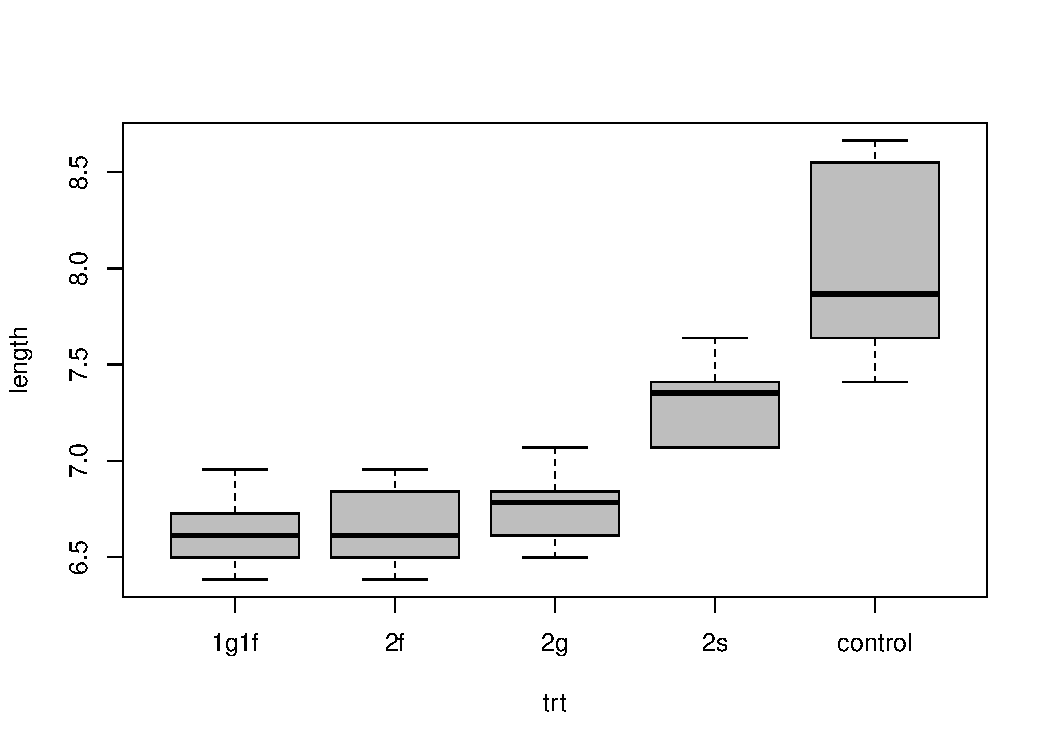
\includegraphics{pea_boxplot}}
\end{center}
\caption{Side-by-side boxplot summarizing data on the growth of pea plants based on different sugar treatments to the soil.}
\label{fig:pea.boxplot}
\end{figure}

There are certain follow-up questions we might like to ask that can't be expressed in terms of a single contrast.  For example, are the means for the four different sugar levels above all the same?  A way to formulate this question is via a hypothesis 
\[ \mu_1 = \mu_2 \quad \text{and} \quad \mu_2 = \mu_3 \quad \text{and} \quad \mu_3 = \mu_4. \]
(This is not the only possible formulation.)  Each one of those equalities above would correspond to a contrast so we might consider to formulate three contrasts and perform a simultaneous test.  That is, define 
\[ \theta_1 = \mu_1 - \mu_2, \quad \theta_2 = \mu_2 - \mu_3, \quad \text{and} \quad \theta_3 = \mu_3 - \mu_4. \]
These three contrasts correspond to three vectors of weights:
\[ w^{(1)} = (1, -1, 0, 0, 0), \quad w^{(2)} = (0, 1, -1, 0, 0), \quad w^{(3)} = (0, 0, 1, -1, 0). \]
Then the question about the four sugar means being equal corresponds to the hypothesis $H_0: \theta_1 = \theta_2 = \theta_3 = 0$.  Hopefully this reminds you of the partial F test from regression.  SAS can handle simultaneous contrasts easily but, to be honest, I don't know how to do it in R; I know how to introduce multiple contrasts but I'm not sure how to get R to pool them together for a simultaneous test.  So I recommend taking a look at the SAS code and output on the website.  

\begin{example}[Pea plants, cont]
...
\end{example}

A point that needs to be made is that not all sets of contrasts can be pooled together like in the above example.  This restriction is mathematical in nature, not so much scientific, and I give the details below for those of you who are interested.  At a high level, the point is that there should be no redundant contrasts in your set.  This is not unlike how, in regression, we run into problems if one of our predictor variables is perfectly correlated with another.  A simple conclusion that comes out of this restriction is that, if there are $T$ treatment levels, then you can pool together at most $T-1$ contrasts; there are still an unlimited number of contrasts to choose from, but there is a fixed limit on how many can be pooled together.  

\begin{quote}
{\em Mathematical details.}  Remember that each contrast corresponds to a vector of weights, and those weights live in a $(T-1)$-dimensional subspace of the full $T$-dimensional space, as a result of the sum constraint.  What is required when considering pooling together of multiple contrasts is that they (or their corresponding weight vectors) be {\em linearly independent}.  A set of $k$ contrasts---$\theta_1,\ldots,\theta_k$---are linearly independent if 
\[ c_1\theta_1 + c_2 \theta_2 + \cdots + c_k \theta_k = 0 \implies c_1 = c_2 = \cdots = c_k = 0. \]
This is just a mathematical representation of the ``no redundant contrasts'' condition.  In other words, there is no way to recover one of the contrasts by taking a linear combination of the others.  As a quick example, let $T=3$ and consider two contrasts 
\[ \theta_1 = \mu_1 - \mu_3 \quad \text{and} \quad \theta_2 = \tfrac12(\mu_1 + \mu_2) - \mu_3. \]
These two are linearly independent and, to see this we multiply each by a constant, add them together, and set equal to 0:
\[ c_1 \theta_1 + c_2 \theta_2 = c_1 (\mu_1 - \mu_3) + c_2 \{\tfrac12(\mu_1 + \mu_2) - \mu_3\} \overset{\text{\tiny set}}{\, = \,} 0. \]
We can do some simplification:
\[ (c_1 + \tfrac{c_2}{2})\mu_1 + \tfrac{c_2}{2} \mu_2 - (c_1 + c_2) \mu_3 \overset{\text{\tiny set}}{\, = \,} 0. \]
The only way that $\mu_2$ doesn't show up on the right-hand side is if $c_2=0$ so we can simplify more:
\[ c_1 (\mu_1 - \mu_3) \overset{\text{\tiny set}}{\, = \,} 0. \]
Since the right-hand side must be 0 for any $\mu_i$'s, the only way we can arrange this is if $c_1=0$ too, so we've shown that $\theta_1$ and $\theta_2$ are linearly independent.  But if we add a third contrast, say, $\theta_3 = \mu_1-\mu_2$, then linear independence fails.  To see this, note that $\theta_1 - \theta_2 + \tfrac12 \theta_3 = 0$.  Anyway, if the $k$ contrasts $\theta_1,\ldots,\theta_k$ are linearly independent, then there is a corresponding contrast sum of squares, $\text{SS}(\theta_1,\ldots,\theta_k)$ and the null hypothesis $H_0: \theta_1 = \cdots = \theta_k = 0$ can be tested with the F statistic 
\[ F = \frac{\text{MS}(\theta_1,\ldots,\theta_k)}{\text{MSE}} = \frac{\text{SS}(\theta_1,\ldots,\theta_k)/k}{\text{MSE}}, \]
where MSE is from the original analysis of variance table.  When we put multiple contrasts all in the same {\tt CONTRASTS} line in the SAS code, it will return to us the results of this F test, including a p-value.  This will fail and SAS will return an error if the contrasts are not linearly independent.  
\end{quote}

There is something interesting that happens if contrasts have a further mathematical property, called {\em orthogonality}.  Remember the original partitioning of the sum of squares was a result of there being a sort of ``right angle,'' or perpendicular lines, and the Pythagorean theorem.  It turns out that if the contrasts have a certain orthogonality property, then there is a further partitioning of the sum of squares.  

\begin{quote}
{\em More mathematical details.}  Let $\theta = \sum_{i=1}^T w_i \mu_i$ and $\theta' = \sum_{i=1}^T w_i' \mu_i$ be two contrasts with weight vectors $w$ and $w'$.  If the design is balanced,\footnote{It is easy to adjust this definition of orthogonality to deal with unbalanced designs where not all of the $r_i$'s are equal.  That is, contrasts $\theta$ and $\theta'$ are orthogonal if $\sum_{i=1}^T r_i^{-1} (w_i w_i') = 0$.} so that there are equal replications in each treatment level, then we say that $\theta$ and $\theta'$ are {\em orthogonal} if $\sum_{i=1}^T w_i w_i' = 0$.  Orthogonality, of course, is a mathematical property that has nothing to do with the scientific context---so the reader should not feel compelled to choose the contrasts they wish to consider based on orthogonality alone.  But it often happens that relevant scientific questions correspond to orthogonal contrasts.  For example, consider the set of contrasts listed in the SAS code for the pea plant growth example above:
\begin{align*}
w^{(1)} & = (0.25, 0.25, 0.25, 0.25, -1) \\
w^{(2)} & = (1, -1, 0, 0, 0) \\
w^{(3)} & = (0, 1, -1, 0, 0) \\
w^{(4)} & = (0, 0, 1, -1, 0).
\end{align*}
These correspond to a question about average of sugars versus control and then some pairwise comparisons among the sugars.  It is easy to check that $w^{(1)}$ is orthogonal to the other three; but the latter three are not orthogonal with each other.  

Why do we care about orthogonality?  There's an interesting property about our analysis of variance that results from following mathematical fact:
\begin{quote}
Let $\theta_1,\ldots,\theta_k$ be a set of linearly independent contrasts and assume that they split into two groups, say, $(\theta_1,\ldots,\theta_m)$ and $(\theta_{m+1},\ldots,\theta_k)$, such that any contrast in one group is orthogonal to any contrast in the other group; they need not be orthogonal within groups.  Then the sum of squares corresponding to the full set of contrasts can be partitioned as follows:
\[ \text{SS}(\theta_1,\ldots,\theta_k) = \text{SS}(\theta_1,\ldots,\theta_m) + \text{SS}(\theta_{m+1},\ldots,\theta_k). \]
\end{quote}
When $k=T-1$, so that the set of contrasts is ``maximal,'' the sum of squares on the left-hand side is SS(Model).  So the above result says that our original partitioning of the total sum of squares---which was the basis for all we've done so far with analysis of variance---can be further partitioned, breaking the model sum of squares down into contributions coming from each set of orthogonal contrasts.  In the pea plant growth example, the contrast corresponding to $w^{(1)}$ above is orthogonal to the other three, and that forms our two groups.  This set of contrasts is maximal because there's $T-1=4$ of them and they're linearly independent.  So we should see that the contrast sums of squares for each of these to add up to the model sum of squares.  And from the SAS output in Figure~\ref{fig:pea.output}, we have 
\[ \text{SS(Model)} \approx 14 \quad \text{and} \quad \begin{cases} \text{SS(``Ctrl vs Avg'')} \approx 10.82 \\ \text{SS(``Sugars'')} \approx 3.18 \end{cases} \]
and, since the two sums of squares on the right add up to the one on the left, we've confirmed what the theory predicted would happen.  
\end{quote}

\begin{figure}[t]
\begin{center}
\scalebox{0.5}{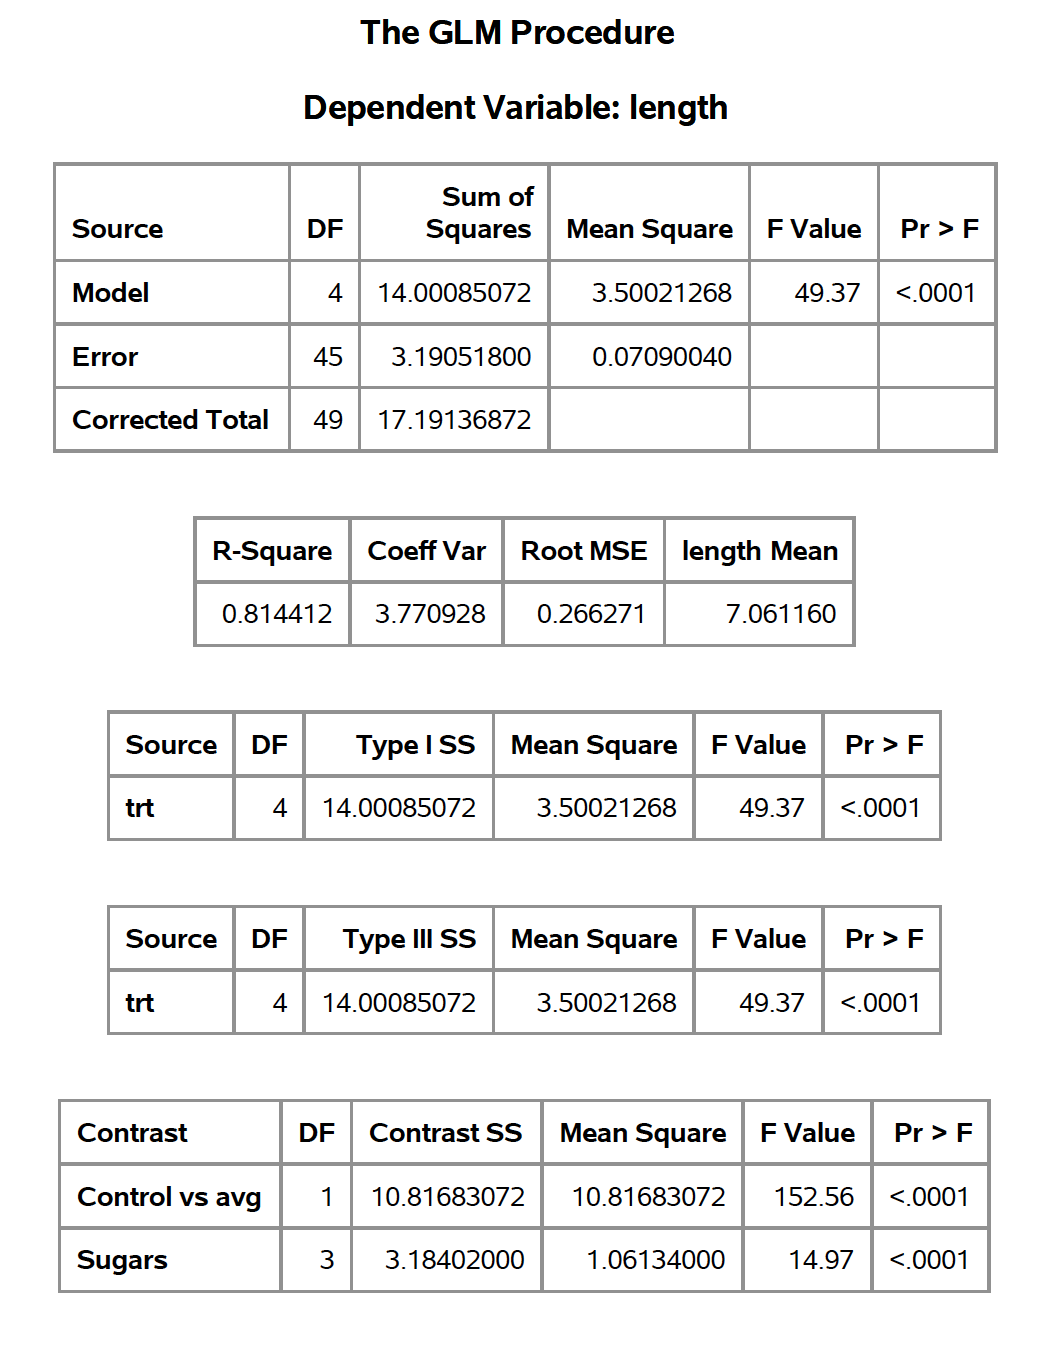
\includegraphics{pea_output}}
\end{center}
\caption{Output from {\tt PROC GLM} for the pea plant growth example.}
\label{fig:pea.output}
\end{figure}

At the moment it likely seems like orthogonality of contrasts has little practical relevance, which is somewhat true.  As we go along, there will be instances where orthogonality plays a role and I'll mention them at least here in these notes even if it's not the best use of time during lectures.  


\subsection*{Extra: Orthogonal contrasts example}

I won't have time to cover this example in class, but it's sufficiently interesting that I want to present the details here in the notes.  Thanks to Professor Kevin Gross for sharing this example with me.  

An experiment is conducted to study the effect of plant row spacing and soybean crop yield.  Here the distance between rows, denoted by {\tt width}, is set at five equally-spaced levels: 18, 24, 30, 36, and 42.  The response variable is {\tt yield}. There are $r=6$ replications at each level of {\tt width}, so there is a total of $n=30$ response variable measurements. The data and SAS code are available on the course website, {\tt spacing.sas}.  A first step is to draw a plot to visualize the relationship between {\tt width} and {\tt yield}.  Figure~\ref{fig:spacing.scatter} shows a plot of {\tt yield} by {\tt width}.  The general pattern here is that as {\tt width} is changed from left to right, the mean {\tt yield} seems to decrease at first and then increase.  An useful feature of this example, which often does not hold for categorical predictor variables, is that the ordering of the {\tt width} levels is meaningful; that is, 24 is really 6 units larger than 18, etc.  So we {\em can}---but don't have to---interpret the relationship in Figure~\ref{fig:spacing.scatter} like we would in a regression setting.  In that light, we see that there is a curved relationship between the two variables, maybe quadratic.  

\begin{figure}[t]
\begin{center}
\scalebox{0.6}{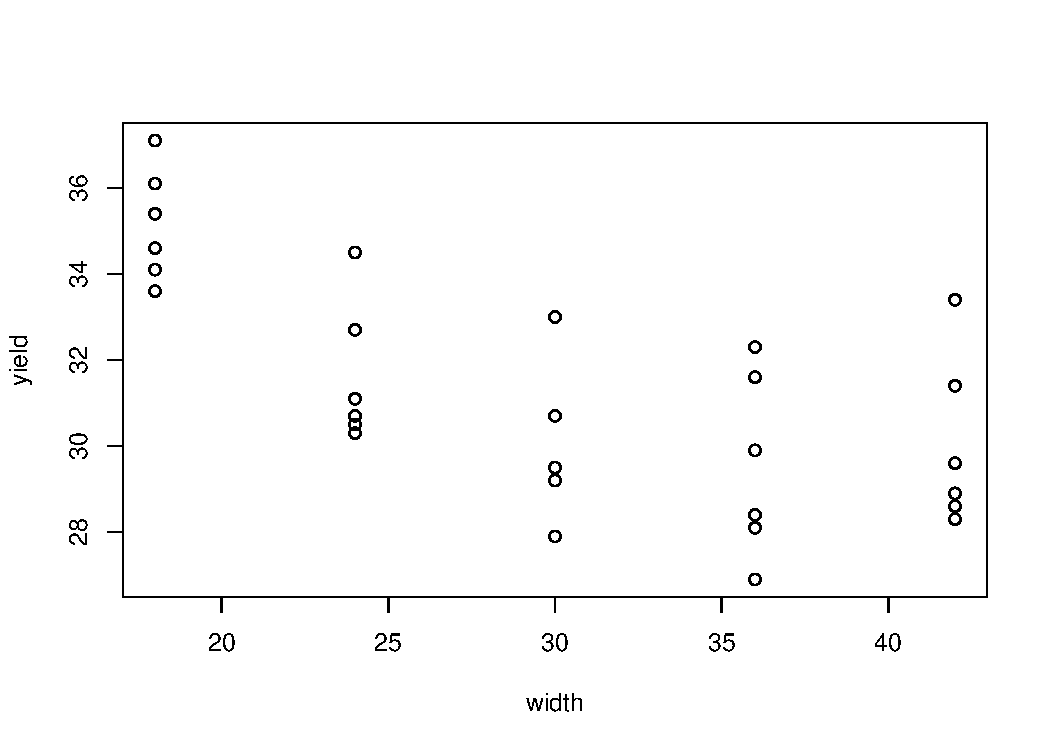
\includegraphics{spacing_scatter}}
\end{center}
\caption{Plot of {\tt yield} versus {\tt width} in the spacings example.}
\label{fig:spacing.scatter}
\end{figure}

Since we have a meaningful ordering of the {\tt width} levels and there seems to be a discernible trend, we have a choice to make: should we treat this like a one-way analysis of variance problem with a categorical predictor, or as a regression problem with a numerical predictor?  Before trying to answer this question, we should first understand why we might consider this in the first place.  Imagine that we did treat this as a regression problem, and that we considered a quadratic model in terms of {\tt width}.  Then to describe the mean structure, we would need three $\beta$ parameters: one intercept, one coefficient on {\tt width}, and one coefficient on ${\tt width}^2$.  Compare this to the one-way analysis of variance model where, sine there are $T=5$ levels, we need five parameters: one baseline mean and four non-zero effects.  So it's actually a simpler model if {\tt width} is treated as a numerical variable in a regression type setting.  How can we tell if this simpler model is adequate?  ({\em Note:} The analysis that follows is applicable only in cases where there are equal replications and the levels of the factor are equally spaced, like here.) 

As the title of this section suggests, orthogonal contrasts will play a role here.  More specifically, we will apply what are called {\em orthogonal polynomial contrasts}.  If we have $T=5$ levels for the {\tt width} factor, then we can decompose the model sum of squares into a sum of four contrast sums of squares, each corresponding to an orthogonal contrast.  Here the four contrasts---labeled ``Linear,'' ``Quadratic,'' ``Cubic,'' and ``Quartic'' in the code and output---are specifically designed to assess whether whether terms of those functional forms are helpful to the model.\footnote{I won't explain where these contrasts come from, but there are references available, e.g., Chapter~4.3 of Oehlert's book, \url{http://users.stat.umn.edu/~gary/book/fcdae.pdf}.}  You can see the contrasts in the SAS code and it is easy to check that they're orthogonal.  Let's check linear and quadratic: 
\[ w_{\text{linear}} = (-2, -1, 0, 1, 2) \quad \text{and} \quad w_{\text{quad}} = (2, -1, -2, -1, 2). \]
Multiplying the corresponding components and summing gives 
\[ %\langle w_{\text{linear}}, w_{\text{quad}} \rangle = 
-2\times 2+(-1)\times(-1)+0\times(-2)+1\times(-1)+2\times2=0, \]
hence, the two contrasts are orthogonal.  Similar verification for the others.  And from SAS output in Figure~\ref{fig:spacing.anova} we can see the sum of squares partitioning:
\begin{align*}
\text{SS(Model)} & = 125.66 \\
& = 91.267+33.693+0.50417+0.197 \\
& = \text{SS}(\theta_{\text{linear}}) + \text{SS}(\theta_{\text{quad}}) + \text{SS}(\theta_{\text{cubic}}) + \text{SS}(\theta_{\text{quartic}}). 
\end{align*}
We see that the cubic and quartic terms contribute only a very small amount to the model sum of squares, which is an indication that they may not be important.  This is confirmed by the large p-values resulting from the corresponding F tests.  Therefore, we conclude that there are no important effects in the cubic and quartic directions, hence only a linear or quadratic model is needed.  

\begin{figure}[t]
\begin{center}
\scalebox{0.5}{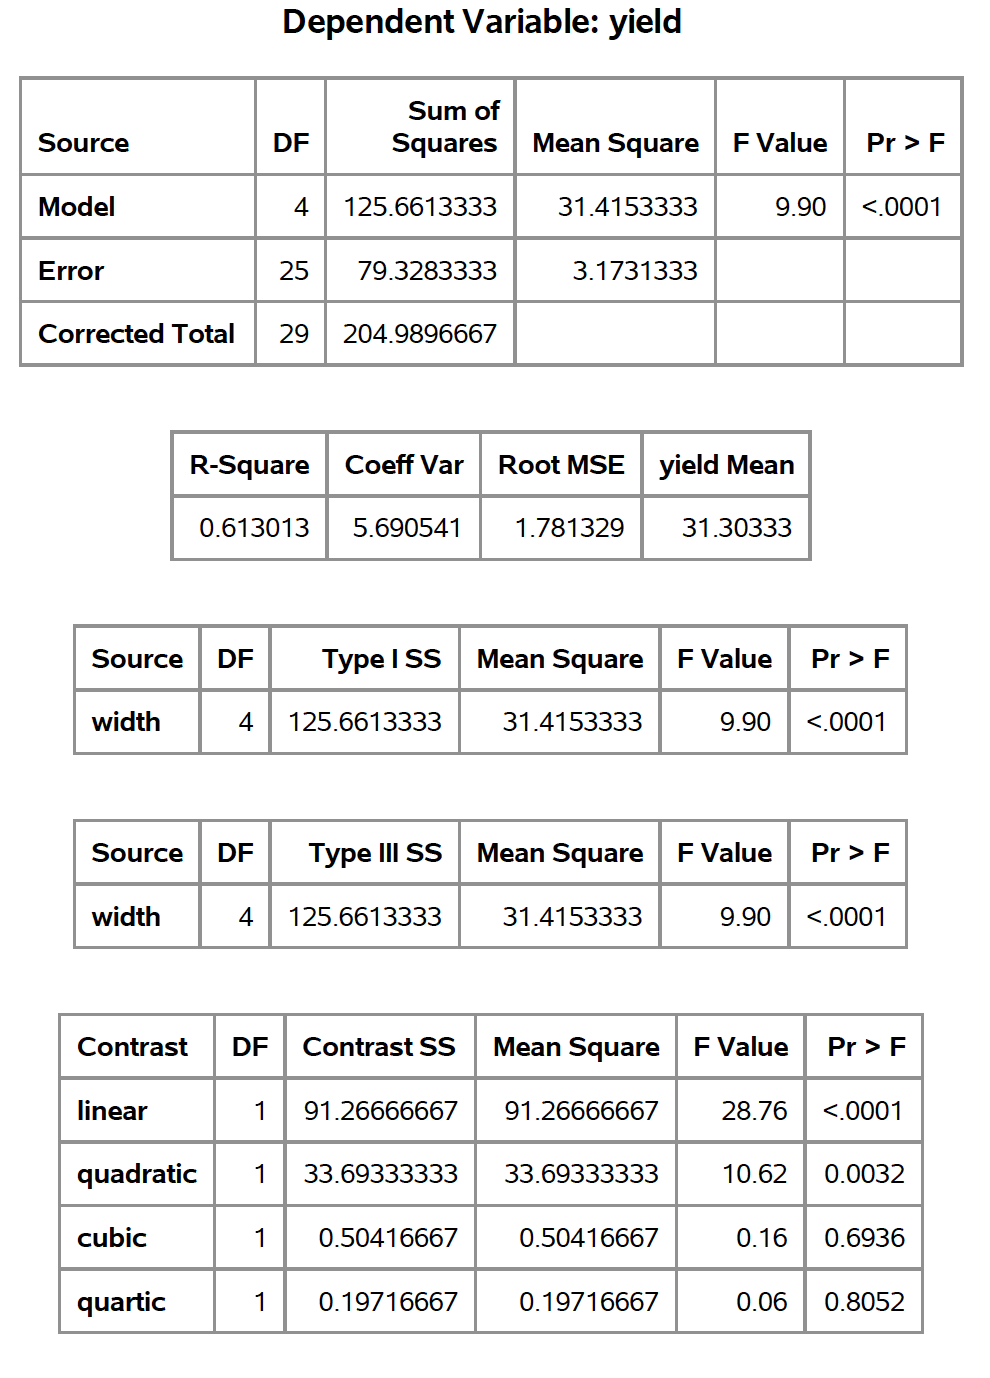
\includegraphics{spacing_anova1}}
\end{center}
\caption{SAS output, with contrasts, for the spacing example.}
\label{fig:spacing.anova}
\end{figure}

If we fit just a quadratic model, then the sum of squares corresponding to cubic and quartic don't disappear, they just get interpreted differently.  Define
\begin{align*}
\text{SS(``Linear'' \& ``Quadratic'')} & = \text{SS(``Linear'')} + \text{SS(``Quadratic'')} \\
\text{SS(``lack of fit'')} & = \text{SS(``Cubic'')} + \text{SS(``Quartic'')}.
\end{align*}
Note that if you add up the sums of squares corresponding to linear and quadratic in the previous output, this equals the model sum of squares in the output corresponding to the quadratic fit in Figure~\ref{fig:spacing.quadratic1}.  This gives a partition of the model sum of squares into a part described by the quadratic model and a part corresponding to a lack of fit. But that latter component now more naturally belongs to a different category.  Going back to our original partitioning of the total sum of squares into a part for the model and a part for error, we can now write 
\[ \text{SS(Total)} = \text{SS(Quadratic Model)} + \text{SS(Lack of Fit)} + \text{SS(Error)}. \]
The discussion in Chapter~11.5 of Ott \& Longnecker on testing for lack of fit in regression is based on this sum of squares partitioning, but they don't present it in terms of orthogonal polynomial contrasts.  Figure~\ref{fig:spacing.quadratic1} also shows estimates of the coefficients in the quadratic model fit, which we can use for prediction at different row widths, etc.  Finally, Figure~\ref{fig:spacing.quadratic2} gives a visualization of the quadratic model fit and we can easily see that the line captures nicely the curvature we say in the original plot of the data above.  

\begin{figure}[t]
\begin{center}
\scalebox{0.5}{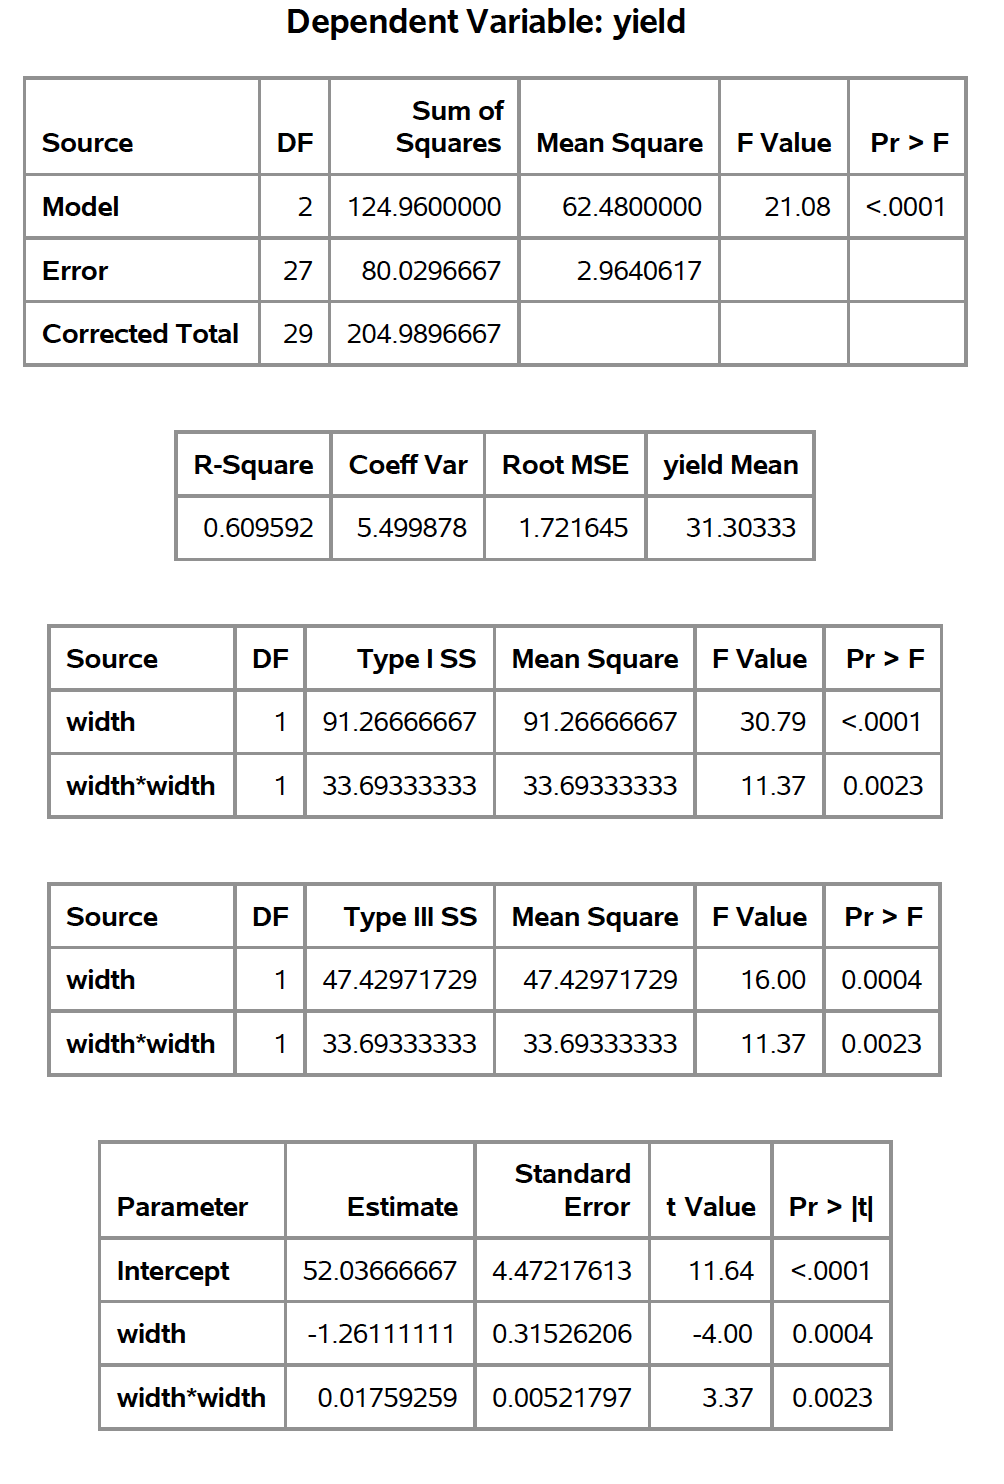
\includegraphics{spacing_anova2}}
\end{center}
\caption{SAS output for the quadratic model fit in spacing example.}
\label{fig:spacing.quadratic1}
\end{figure}

\begin{figure}[t]
\begin{center}
\scalebox{0.35}{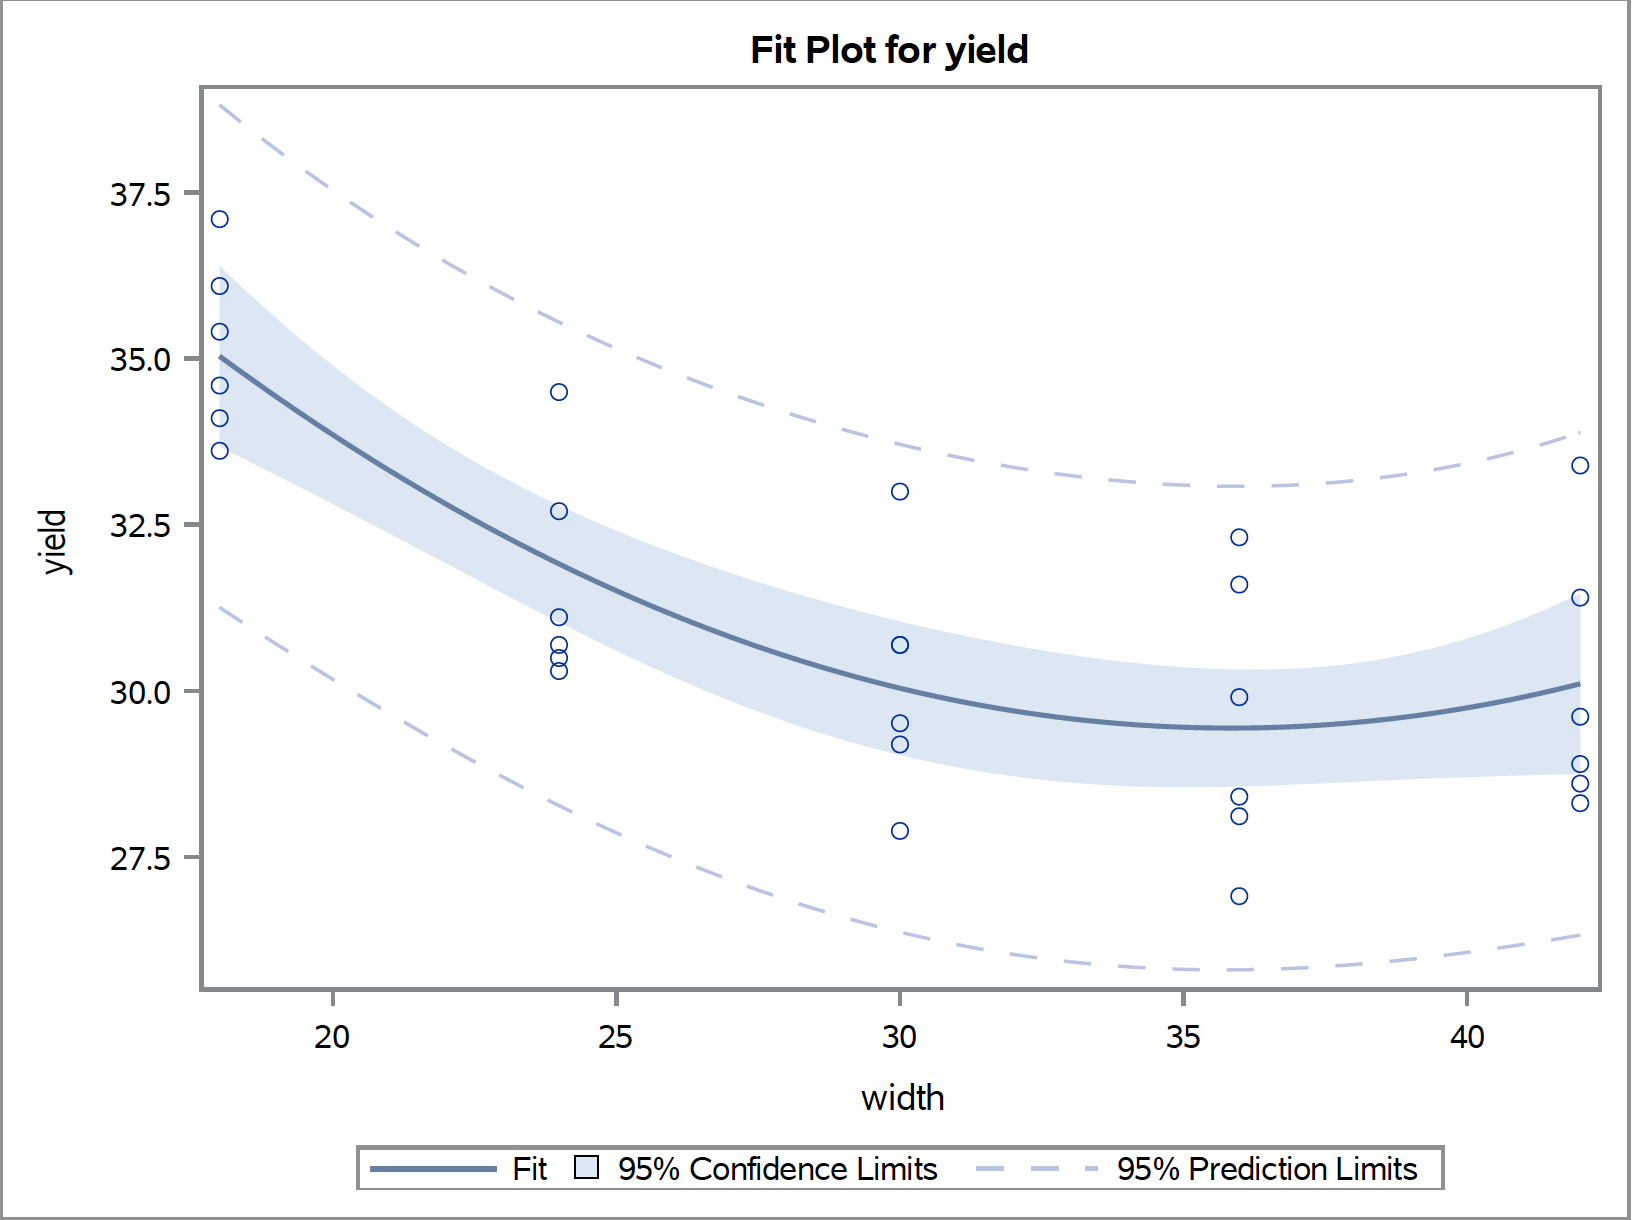
\includegraphics{spacing_quad}}
\end{center}
\caption{Visualization of the quadratic model fit in spacing example.}
\label{fig:spacing.quadratic2}
\end{figure}


\ifthenelse{1=1}{}{

This exercise is based on an example that I wanted to go through in class, but ran out of time.  Here I walk you through the steps; see my SAS codes in the file {\tt spacings.sas}.  This problem won't be graded, but I hope you'll go through it since there's some take-away points that I think are interesting/useful.  

An experiment is conducted to study the effect of plant row spacing and soybean crop yield.  Here the distance between rows, denoted by {\tt width}, is set at five equally-spaced levels: 18, 24, 30, 36, and 42.  The response variable is {\tt yield}.  
\begin{enumerate}
\item Draw a plot of {\tt yield} versus {\tt width}.  Do you think there is any difference between the mean yields at the different row widths?
\item Carry out a formal test to justify the claim that the mean yields are not all the same across row widths.  
\item Since {\tt width} is actually a numerical variable, it might make sense to treat this like a regression problem instead of one-way analysis of variance.  A reason for doing so might be to get a simpler explanation of the relationship between {\tt width} and {\tt yield}, i.e., instead of having 5 mean parameters, maybe we only need a one or two ``$\beta$'s'' to describe a linear/curved relationship.  Based on the plot in Part~(a), if you think of {\tt width} as a numerical variable, what kind of relationship with {\tt yield} do you see?  
%(\emph{and the levels are equally spaced with equal number of replications}), 
\item {Since the levels of {\tt width} are equally spaced, with the same number of replications per level}, we can assess the adequacy of a curved relationship between {\tt width} and {\tt yield} based on \emph{orthogonal polynomial contrasts}.  In the SAS code, you see four CONTRAST statements, labeled ``Linear,'' ``Quadratic,'' ``Cubic,'' and ``Quartic,'' which are specifically designed\footnote{I won't explain where these contrasts come from, but there are references available, e.g., Chapter~4.3 of Oehlert's book, \url{http://users.stat.umn.edu/~gary/book/fcdae.pdf}.} to assess whether those functional forms are helpful to the model.  
\begin{enumerate}
\item Verify that the four contrasts listed in the code are, indeed, orthogonal.  
\item In the SAS output, verify that the sums of squares for these four contrasts add up to the sum of squares for the model in Part~(b) above.
\end{enumerate}
\item Using the F-tests for the individual contrasts, justify the claim that the ``Cubic'' and ``Quartic'' terms are unnecessary.  Compute 
\begin{align*}
SS(\text{``Linear'' \& ``Quadratic''}) & = SS(\text{``Linear''}) + SS(\text{``Quadratic''}) \\
SS(\text{``lack of fit''}) & = SS(\text{``Cubic''}) + SS(\text{``Quartic''}).
\end{align*}
This gives a partition of the model sum of squares into a part described by the quadratic model and a part corresponding to a lack of fit.  
\item Fit the quadratic model directly by treating {\tt width} as a numerical variable.  Compare the model sum of squares in the new analysis of variance table with the $SS(\text{``Linear'' \& ``Quadratic''})$ you calculated above.  

In this case, the $SS(\text{``lack of fit''})$ above is being included in $SS(\text{Error})$, i.e., the overall error sum of squares in this output partitions into a ``pure error'' part and a ``lack of fit'' part.  The discussion in Chapter~11.5 of Ott \& Longnecker on lack of fit testing in regression is based on this partitioning of $SS(\text{Error})$.  
\end{enumerate}


\begin{itemize}
\item[(a)] From the plot below, it does appear that there is difference between the mean yields at the different row widths.
\begin{figure}[ht!]
\centering
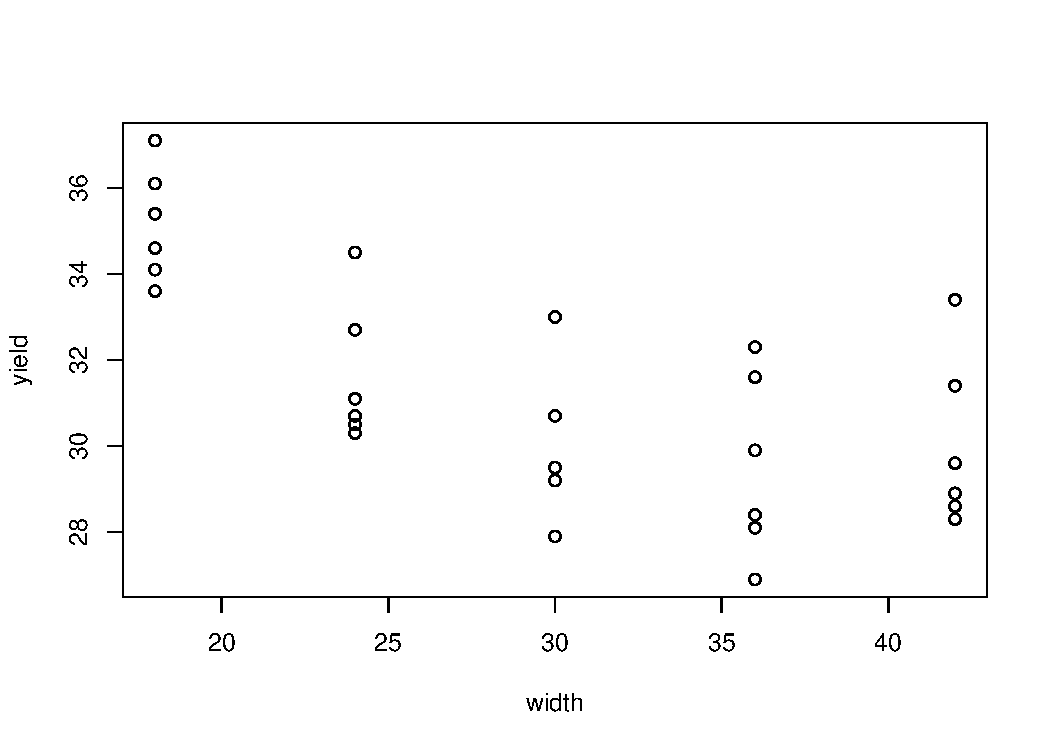
\includegraphics[width=0.6\textwidth]{spacing_scatter.png}
\end{figure}
\item[(b)] First, we write the model as 
\[ y_{ij}=\mu+\tau_i+\epsilon_{ij}, \quad i=1,\ldots,5, \quad j=1,\ldots,6. \] 
The test is equivalent to test $\tau_i=0$ for all $i$ and, from the SAS output (not shown), the F value is 9.9 and the p-value is very small, so we reject the null hypothesis and consider the mean yields are not all the same across row widths.
\item[(c)] Based on the plot above, it looks like maybe a quadratic relationship.  
\item[(d)]
\begin{itemize}
\item[i.] Let's use linear and quadratic for example: 
\[ w_{\text{linear}} = (-2, -1, 0, 1, 2) \quad \text{and} \quad w_{\text{quad}} = (2, -1, -2, -1, 2). \]
Multiplying the corresponding components and summing---in mathematics, this is called ``inner-product''---gives 
\[ \langle w_{\text{linear}}, w_{\text{quad}} \rangle = -2\times 2+(-1)\times(-1)+0\times(-2)+1\times(-1)+2\times2=0, \]
hence, the two contrasts are orthogonal.  Similar verification for the others.
\item[ii.] We can verify this simply by calculation:
\begin{align*}
\text{SS(Model)} & = 125.66 \\
& = 91.267+33.693+0.50417+0.197 \\
& = \text{SS}(\theta_{\text{linear}}) + \text{SS}(\theta_{\text{quad}}) + \text{SS}(\theta_{\text{cubic}}) + \text{SS}(\theta_{\text{quartic}}). 
\end{align*}
\end{itemize}
\item[(e)] From the SAS output (not shown), we get $F_{\text{cubic}} = 0.16$ and $F_{\text{quartic}} = 0.06$, both of which have small p-values, indicating that the cubic and quartic terms are unnecessary. Lumping ``Linear \& Quadratic'' into a group and ``Cubic \& Quartic'' into a group, the calculation in Part~(d) gives a partition of the model sum of squares into a component corresponding to the linear and quadratic parts, and another part that can be called ``lack of fit.''  
\item[(f)] The model sum of squares in the SAS output for the new quadratic model is exactly the same as $\text{SS}(\theta_{\text{linear}}, \theta_{\text{quad}}) = \text{SS}(\theta_{\text{linear}}) + \text{SS}(\theta_{\text{quad}})$ above.  
\end{itemize}

}


\subsection*{03/05/2019}

\subsubsection*{Adjustments for multiple comparisons}

Contrasts are designed specifically for (follow-up) questions about the treatment level means that were formulated even before the data were analyzed.  For example, pairwise comparisons of new fertilizers with a control.  But when the follow-up questions are more exploratory in nature, e.g., {\em the overall F test says there's differences between treatment level means, but where are the differences?}, some additional care is needed, and this comes in the form of certain adjustments, as I describe below.  

When we want to consider all possible pairs of treatment level means, what we're doing is basically carrying out lots of distinct hypothesis tests.  That is, we aim test test 
\[ H_0^{(i,j)}: \mu_i = \mu_j \quad \text{for all pairs $(i,j)$ of the $T$ levels}. \]
In this case, there are potentially a lot of tests to consider.  In particular, if there are $T$ treatment levels, then the number of hypotheses above to be tested can be evaluated by the formula 
\[ \binom{T}{2} = \text{``$T$ choose 2''} = \text{\# of distinct pairs out of $T$} = \frac{T(T-1)}{2}. \]
For example, if $T=5$ as in the pea plant growth example above, then there are 10 pairs and, therefore, 10 hypotheses to be tested.  OK, fine, we need to do a number of pairwise tests.  Why does it matter how many tests are being considered?

From ST511 you know that the decision to reject a null hypothesis when $\text{p-value} < \alpha$ is based on theory that says such a decision rule will commit a Type~I error\footnote{Recall, a Type~I error is rejecting the null hypothesis when it's true; a Type~II error is not rejecting a null hypothesis when it's false.} with probability $\alpha$.  So by making $\alpha$ reasonably small, e.g., $\alpha=0.05$, we have some assurance that a Type~I error will not be committed, which suggests that the testing method is reliable in some sense.  At least when applied to only a single testing problem.  But if we propose to test, say, 10 hypotheses, then we'd want our procedure to be reliable in a sense that's relevant for the 10 tests together, not just for individual tests.  So what we might consider to be a ``mistake'' in the context of 10 simultaneous hypothesis tests is 
\[ \text{\em at least one Type I error is committed}. \]
Unfortunately, equipping each individual test with a certain degree of Type~I error control does not imply the same amount of control on errors of the form above.  Indeed, if we carry out $m$ test simultaneously, all having Type~I error probability $\alpha$, and if all the $m$ tests are {\em independent},\footnote{I'll not get into formal details about independence here, but this basically boils down to the tests being based on distinct subsets of the data.  For the present context of pairwise comparisons, an independence assumption {\em does not} hold, but this specific calculation is just for illustration; and the fact that our pairwise comparisons are not independent doesn't mean that the problems associated with multiplicity are absent, only that they're harder to characterize/understand.} then it is pretty easy to show that 
\[ \prob(\text{at least one Type~I error}) = 1 - (1-\alpha)^m. \]
The quantity on the left-hand side is called the {\em family-wise error rate}.  It is also pretty easy to see that, if $m > 1$, then the right-hand side above is bigger than $\alpha$.  Figure~\ref{fig:fwer} shows a plot of the right-hand side above, as a function of $m$, for $\alpha=0.05$.  As you can see, this is increasing quite rapidly in $m$ so that, even with just $m=10$ tests, the probability of at least one Type~I error is about 0.40!  And if there's a 40\% chance we make at least one Type~I error, then conclusions we draw based on our series of tests cannot be reliable.  

\begin{figure}[t]
\begin{center}
\scalebox{0.65}{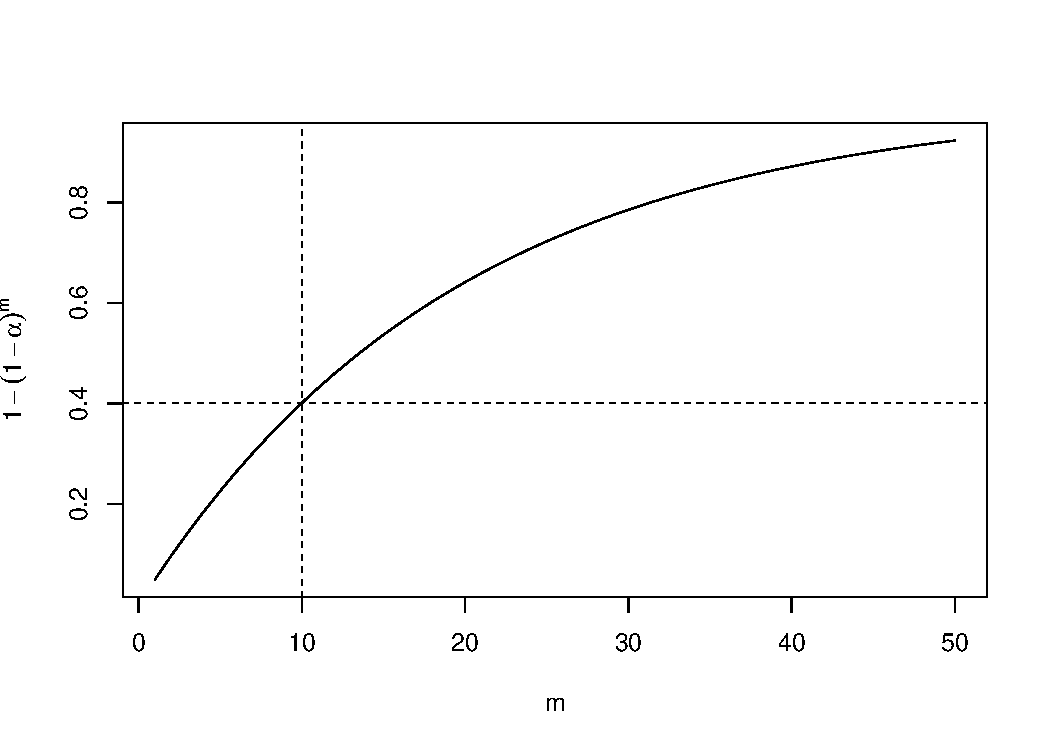
\includegraphics{fwer}}
\end{center}
\caption{Plot of the family-wise error rate, $m \mapsto 1-(1-\alpha)^m$, for $\alpha=0.05$.}
\label{fig:fwer}
\end{figure}

One possible remedy is to adjust the $\alpha$ level for each individual test, i.e., to shrink the level from $\alpha$ to some $\alpha' < \alpha$ so that $1-(1-\alpha')^m$ is no larger than the target family-wise error rate.  This is a good idea, but what should $\alpha'$ be?  The simplest adjustment is called the {\em Bonferroni correction} and it goes as follows.  If we want to carry out $m$ tests, and we want our family-wise error rate to be no more than $\alpha$, then we should take $\alpha' = \alpha / m$.  The proof that this correction works is based on an elementary probability inequality:
\[ \prob(\text{at least one Type~I error}) \leq \sum_{i=1}^m \prob(\text{Type I error on test $i$}) = m\alpha' = \alpha. \]
The downside to such an adjustment is that, using the smaller $\alpha'$ to perform each test makes it harder to reject, i.e., a larger difference between $\hat\mu_i$ and $\hat\mu_j$ is needed to conclude that the corresponding means are significantly different.  In other words, multiplicity corrections make the individual tests more conservative and, hence, there is a loss of power.  Some kind of additional conservatism is necessary when carrying out multiple tests simultaneously, but there are more sophisticated methods that do better than the simple Bonferroni adjustment described above.  One that Ott \& Longnecker discuss is {\em Tukey's method}, but there are others.  We'll be able to use these more sophisticated methods, such as Tukey's, even if we haven't gone through the technical details.  In SAS, by adding a {\tt MEANS} line in the PROC GLM code, with an option {\tt BON} (or {\tt TUKEY}) then we can get the results of such methods.  They all return a grouping of the different means based on which ones are not significantly different according to the specified testing rule.  

A hot topic in statistics research over the past 10 years or so has been situations where the goal is to carry out perhaps thousands of tests simultaneously.  Besides being theoretically interesting, my understanding is that there are real scientific problems where this kind of problem arises and statistical methods to handle them are needed.  I don't know anything about the actual science, but I did some work on the statistical side of these large-scale multiple testing problems.  I won't discuss these technicalities in lecture but, if you're interested, feel free to ask and we can talk outside of class. 


\begin{remark}
There's some inconsistency in terms of the emphasis placed on corrections for multiplicity.  For example, in the pairwise comparison context considered here, any statistician would recommend the use of some kind of multiplicity correction.  However, as we've described throughout the course, we do one test (e.g., overall F test) and then proceed to carry out additional tests according to the relevant scientific follow-up questions.  That is, we're almost always doing ``multiple tests'' and, in those cases, we don't normally consider making multiplicity adjustments.  Personally, I'm on the fence about this: on one hand, my belief is that the logic of statistical inference relies almost exclusively on the notion of reliability discussed above, so it's hard for me to accept the possibility that error rates are not being controlled; on the other hand, trying to correct for all possible multiplicities would be more of a handicap than a benefit.  So until I have something better to recommend, I'll bite my tongue about the loss of reliability risk in those typical cases as we've been considering throughout the course.  
\end{remark}


\subsubsection*{Factorial designs for two factors}

The situation considered so far is where there was only one variable, what we referred to as {\em treatment}, and we decided (via randomization) which units were assigned to the different treatment levels.  But one can easily imagine situations where more than one variable might be of interest.  Henceforth, we will refer to these variables as {\em factors} and, shortly, I will make clear the connection between factors and treatment.  I will refer to factors by upper-case letters A, B, C, and so forth.  To start, we'll consider the case of two factors, A and B, and the extension to more than two factors from there will be clear.  

With a single factor, under a completely randomized design, we visualized the structure by drawing a line---a one-dimensional array---of cells and then the experimental units were randomly allocated to the cells.  Now that we have two factors at play, it makes sense that the visualization would be based on a two-dimensional array, with rows corresponding to the levels of factor A and columns corresponding to the levels of factor B.  If we label the factor A levels as $1,2,\ldots,a$ and the factor B levels as $1,2,\ldots,b$, then this would be an $a \times b$ array; see Figure~\ref{fig:twoway}.  Then to each of the $ab$ cells in that table, the experimental units are randomly allocated just like before.  For now, I'll also assume that the design is {\em balanced} in the sense that an equal number, say $r$, of replications are assigned to each cell.  Therefore, we need at least $rab$ experimental units to fill all the cells with $r$ many units.  This design, which is called a (balanced) {\em two-way factorial design}.  This is a ``gold-standard'' design in the sense that it is sufficiently rich that we can estimate all the necessary parameters.  There will be other cases when, perhaps due to resource limitation, a full factorial design like this is not possible, so some sacrifices about what can be estimated are needed; this is more complicated but I might at least mention something about this later.  

\begin{figure}[t]
\begin{center}
\scalebox{0.55}{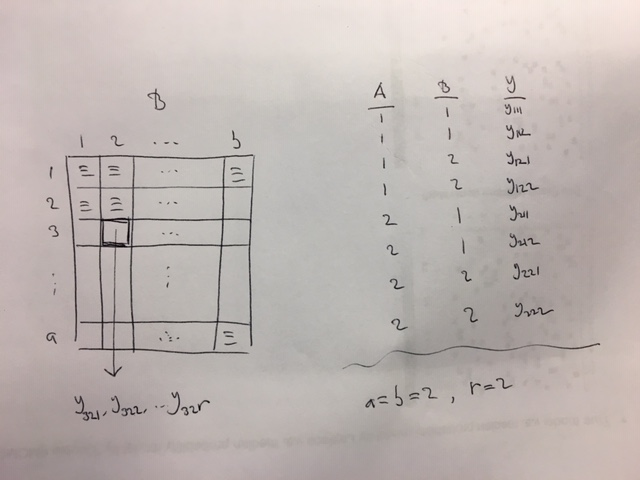
\includegraphics{IMG_0071.jpg}}
\end{center}
\caption{Two-way factorial design layout and spreadsheet form.}
\label{fig:twoway}
\end{figure}

The design is called ``factorial'' because the treatments are made up of combinations of the different factor levels.  In the case of one factor, there was no need to distinguish between the factor and treatment, because they were the same.  In this case, however, the treatments correspond to cells in the two-way arrangement, and the cells correspond to combinations of A and B factor levels.  Therefore, it makes sense now to distinguish between factor and treatment.  


\subsection*{03/07/2019}

Like in the one-way case, there is a mean parameter corresponding to each treatment, in this case, each cell.  Since we refer to cells by their row and column labels, we need two subscripts to denote the means: $\mu_{ij}$ denotes the mean response for units assigned to level $i$ of factor A and level $j$ of factor B so, altogether, there are $ab$ total mean parameters.  These means can easily be estimated by calculating the average of the $r$ replicates within each cell; that is, the estimate, $\hat\mu_{ij}$, of $\mu_{ij}$ is just the average of $y_{ij1},\ldots,y_{ijr}$, and SAS's PROC MEANS will do this calculation for us.  But in situations with two factors under consideration, often the primary objective is to understand how the factor levels simultaneously influence the mean response, but these summary statistics don't help in that direction.  To deal with this more complicated question, we need to formulate a statistical model.  

As in the one-way case, the model in terms of the cell means is the simplest to state but not really helpful to analyze.  That is, the means model says 
\[ y_{ijk} = \mu_{ij} + \eps_{ijk}, \quad \begin{cases} i=1,2,\ldots,a \\ j = 1,2,\ldots,b \\ k=1,2,\ldots,r, \end{cases} \]
where $\eps_{ijk}$ satisfy the same assumptions as before, namely, independent, normally distributed, with mean 0 and variance $\sigma_\eps^2$ that does not depend on $(i,j,k)$.  But, again, this version of the model doesn't isolate the effects of A, of B, or of some ``joint'' A--B effect.  So we can expand on the overly-simple model above as follows:
\[ \mu_{ij} = \mu + \alpha_i + \beta_j + (\alpha\beta)_{ij}. \]
That is, the cell means can be expressed in terms of a baseline mean, an effect of level $i$ of factor A, an effect of level $j$ of factor B, and a joint effect of the cell $(i,j)$ of A--B.  The latter is called the {\em interaction} effect, which is often of primary interest; see below.  It is worth to point out that $(\alpha\beta)_{ij}$ does not correspond to the product of $\alpha_i$ and $\beta_j$, it is a separate symbol that represents the joint effect of the $(i,j)$ levels of factors A and B, hence the concatenation of ``$\alpha$'' and ``$\beta$.''  

There are a lot of these effects parameters, but they can be estimated using PROC GLM just like as we've seen before.  In the code, however, we have to tell SAS if we want to include the interaction term or not.  There's a couple ways that we can do it, one is a shortcut for the other.  If the two factors are labeled as {\tt A} and {\tt B} in the data set, and the response is {\tt y}, then to fit the full two-way interaction model in PROC GLM, either one of the following model statements would suffice:
\[ \text{\tt model y = A B A*B;} \quad \text{or} \quad \text{\tt model y = A | B;} \]
That is, the vertical bar ``{\tt |}'' tells SAS to include {\tt A}, {\tt B}, and their interaction, which is a shortcut to writing out all three of the terms manually.  When we have more than two factors, the vertical bar shortcut saves more time.  

The first step in analyzing data relative to this model is, as we've discussed a number of times before, to determine if there's anything interesting going on at all, i.e., if there is any differences across the treatment means, the $\mu_{ij}$'s.  For this, we have an overall F test.  That is, if the goal is to test the hypothesis 
\[ H_0: \text{all $\mu_{ij}$'s are the same} \]
or, equivalently, 
\[ H_0: \text{all of $\alpha_i$'s, $\beta_j$'s, and $(\alpha\beta)_{ij}$'s equal zero}, \]
then we can look to the first analysis of variance table in the PROC GLM output.  If that p-value is small, as it often will be, then we can conclude that the hypothesis that nothing interesting is going on is implausible, and we can proceed to ask more precise follow-up questions.  

\begin{example}[14-6 in Ott \& Longnecker]
This example considers two factors, pesticide ($a=4$ levels) and citrus plant variety ($b=3$ levels); the design is a full two-way factorial with $r=2$ replications per factor level combination so, altogether, there are $n=24$ experimental units, i.e., trees.  The response is the fruit yield from each tree.  The scientific goal is to understand how the mean fruit yield is related to the pesticide type and plant variety.  The first basic question is to determine if there is any difference across the combinations of the two factors and, for this, we can carry out an overall F test.  From the PROC GLM output in Figure~\ref{fig:factorial.anova}, we find that the p-value for the overall F test is very small, which indicates that, yes, there is some difference in the mean fruit yields across the different combinations of pesticide and variety.  
\end{example}

\begin{figure}[t]
\begin{center}
\scalebox{0.55}{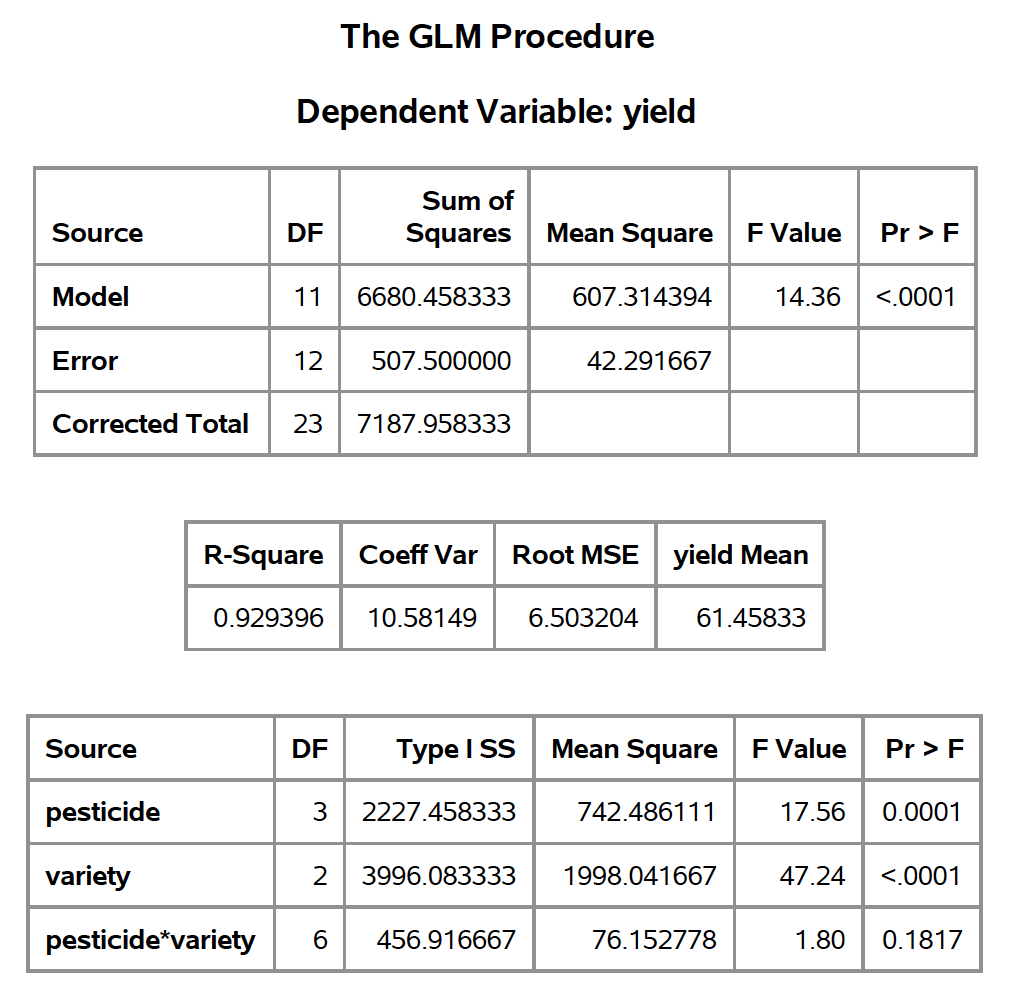
\includegraphics{factorial_output.png}}
\end{center}
\caption{PROC GLM output for Example~14-6 in Ott \& Longnecker.}
\label{fig:factorial.anova}
\end{figure}

When the overall F test rejects, like in the above example, we are in a position to ask some additional follow-up questions about how the treatment means differ.  As hinted at above, the question of primary interest concerns the interaction term in the model, and here's why.  The presence of interaction in the model implies that there's something special about particular combinations of the factor A and B levels, i.e., that the ``best'' treatment isn't necessarily just the combination of the ``best'' levels of factors A and B, respectively.  For example, interaction suggests that changing from level 1 to 2 of factor A could {\em increase} the mean response under level 1 of factor B, but {\em decrease} the mean response under level 2 of factor B.  Since interaction tells us something potentially relevant about the relationship between factors A and B, a natural follow-up question is if interaction is needed.  

Before discussing the formal test about interaction, I want to give some more details about the above relationship between the mean responses when interaction is and isn't present in the model.  For this, lets consider the simplest setup of a $2 \times 2$ factorial design, i.e., $a=b=2$.  In this case, there are four mean responses: $\mu_{11}$, $\mu_{12}$, $\mu_{21}$, and $\mu_{22}$.  Assuming, first, that there's {\em no interaction}, the model (with SAS's choice of level 2 as baseline) says the mean responses can be expressed as 
\begin{align*}
\mu_{11} & = \mu + \alpha_1 + \beta_1 \\
\mu_{12} & = \mu + \alpha_1 + 0\\
\mu_{21} & = \mu + 0 + \beta_1 \\
\mu_{22} & = \mu + 0 + 0
\end{align*}
So if we look at the how the mean response changes when we move from (the baseline) level 2 to level 1 of factor B, at each level of factor A, we find that 
\begin{align}
\mu_{11} - \mu_{12} & = (\mu + \alpha_1 + \beta_1) - (\mu +\alpha_1) = \beta_1 \tag{$B=1$} \\
\mu_{21} - \mu_{22} & = (\mu + \beta_1) - \mu = \beta_1 \tag{$B=2$}
\end{align}
This says that the change in mean response, when we move from (the baseline) level 2 to level 1 of factor A, is the same---equal to $\beta_1$---for both levels of factor B.  That this difference is constant implies that the lines in the {\em interaction plot}, also sometimes referred to as the {\em profile plot}, are parallel; see Figure~\ref{fig:interaction.drawing} (left).  The plot that determines with certainty whether interaction is present or absent is based on the true $\mu_{ij}$ values, which are unknown to us; however, if we draw the corresponding plot with the estimates, the $\hat\mu_{ij}$'s, which SAS does as part of the PROC GLM output when the model has two factors, and if we see roughly parallel lines, then that's an indication that interaction may not be necessary.  A formal test will be discussed below.  

\begin{figure}[t]
\begin{center}
\scalebox{0.55}{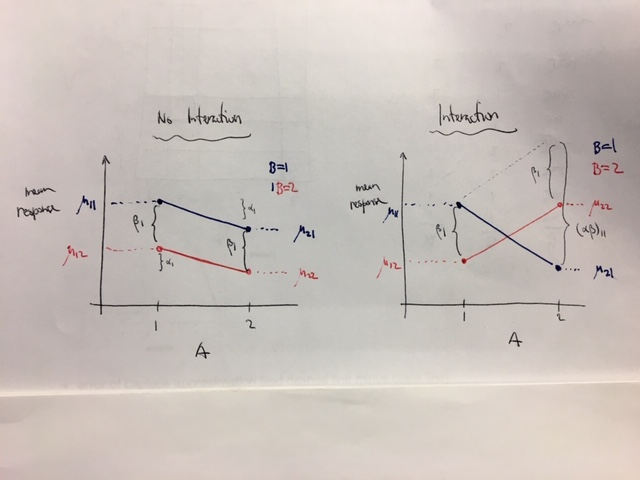
\includegraphics{IMG_0072.jpg}}
\end{center}
\caption{Profile plot when interaction is absent (left) and present (right).}
\label{fig:interaction.drawing}
\end{figure}

A next question is what happens in the above $2 \times 2$ example if there {\em is interaction}.  In that case, the model is slightly more complicated, i.e., using SAS's choice of baseline, 
\begin{align*}
\mu_{11} & = \mu + \alpha_1 + \beta_1 + (\alpha\beta)_{11} \\
\mu_{12} & = \mu + \alpha_1 + 0\\
\mu_{21} & = \mu + 0 + \beta_1 \\
\mu_{22} & = \mu + 0 + 0
\end{align*}
Then the same calculations as above give
\begin{align}
\mu_{11} - \mu_{12} & = \{\mu + \alpha_1 + \beta_1 + (\alpha\beta)_{11}\} - (\mu +\alpha_1) = \beta_1 + (\alpha\beta)_{11} \tag{$B=1$} \\
\mu_{21} - \mu_{22} & = (\mu + \beta_1) - \mu = \beta_1 \tag{$B=2$}
\end{align}
Notice now that the two differences are not the same, which explains why the lines in Figure~\ref{fig:interaction.drawing} (right) are not parallel.  Also, the difference between the two differences is controlled by the interaction term, $(\alpha\beta)_{11}$.  Therefore, when interaction is present, the change in the mean response, when we move from (the baseline) level 2 to level 1 of factor A, is different depending on whether we're in level 1 or 2 of factor B.  And if we see an interaction plot in the PROC GLM output with lines that are not parallel, then that's an indication that interaction is present.  

The next question is how to formally test for the presence of interaction.  This is important for two reasons: first, if interaction is present, then it means we need to consider the factor level settings jointly when trying to determine a ``best'' treatment; and, second, if interaction is not present, then we can remove it from the model which will reduce the number of parameters, improve the accuracy of the error variance estimation, and make the model simpler/easier to interpret.  The scientific question---is interaction important---can be stated statistically as the hypothesis
\[ H_0: \text{all the $(\alpha\beta)_{ij}$'s equal 0}. \]
For this, as you might anticipate, there's a corresponding F test.  In the PROC GLM output, there's a couple tables that display sums of squares, etc, for the two factors and their interaction.\footnote{These tables have ``Type I SS'' and ``Type~III SS,'' respectively, and at the moment they contain identical sets of numbers.  The numbers are the same because we're considering only {\em balanced} factorial experiments; if the design is unbalanced, then the Type~I and Type~III sums of squares will be different, and I'll explain this difference later.}  The F test about the presence of interaction is in the row corresponding to the interaction; we can just read off the F statistic and p-value as usual and, if the p-value is small, then we can conclude that the null hypothesis above is implausible and reject, otherwise, it's sufficiently plausible and we don't reject.  

\begin{example}[14-6 in Ott \& Longnecker, cont]
The interaction plot for this example is shown in Figure~\ref{fig:factorial.interaction}.  Keep in mind, the points where the line segments join are {\em not} the true mean, these are estimates.  So we don't expect to see perfectly parallel lines,\footnote{Note that ``parallel'' is only defined for straight lines, whereas the lines in these interaction plots are typically not straight, they often have kinks.  So when I refer to lines in an interaction plot as being ``parallel'' or not, I mean the individual line segments.} even if interaction is genuinely absent.  In this case, the lines are ``close'' to parallel, which suggests that perhaps interaction is not present in this case.  To carry about the formal test, go to the bottom part of the PROC GLM output displayed in Figure~\ref{fig:factorial.anova}, where we find the sum of squares, etc., for the interaction.  The p-value is about 0.18 which is relatively large, so we conclude that the null hypothesis of no interaction is not so implausible, so we cannot reject.  This confirms the finding based on the interaction plot.  Hence, a simpler model that excludes the interaction term seems to be a better choice.  
\end{example}

\begin{figure}[t]
\begin{center}
\scalebox{0.35}{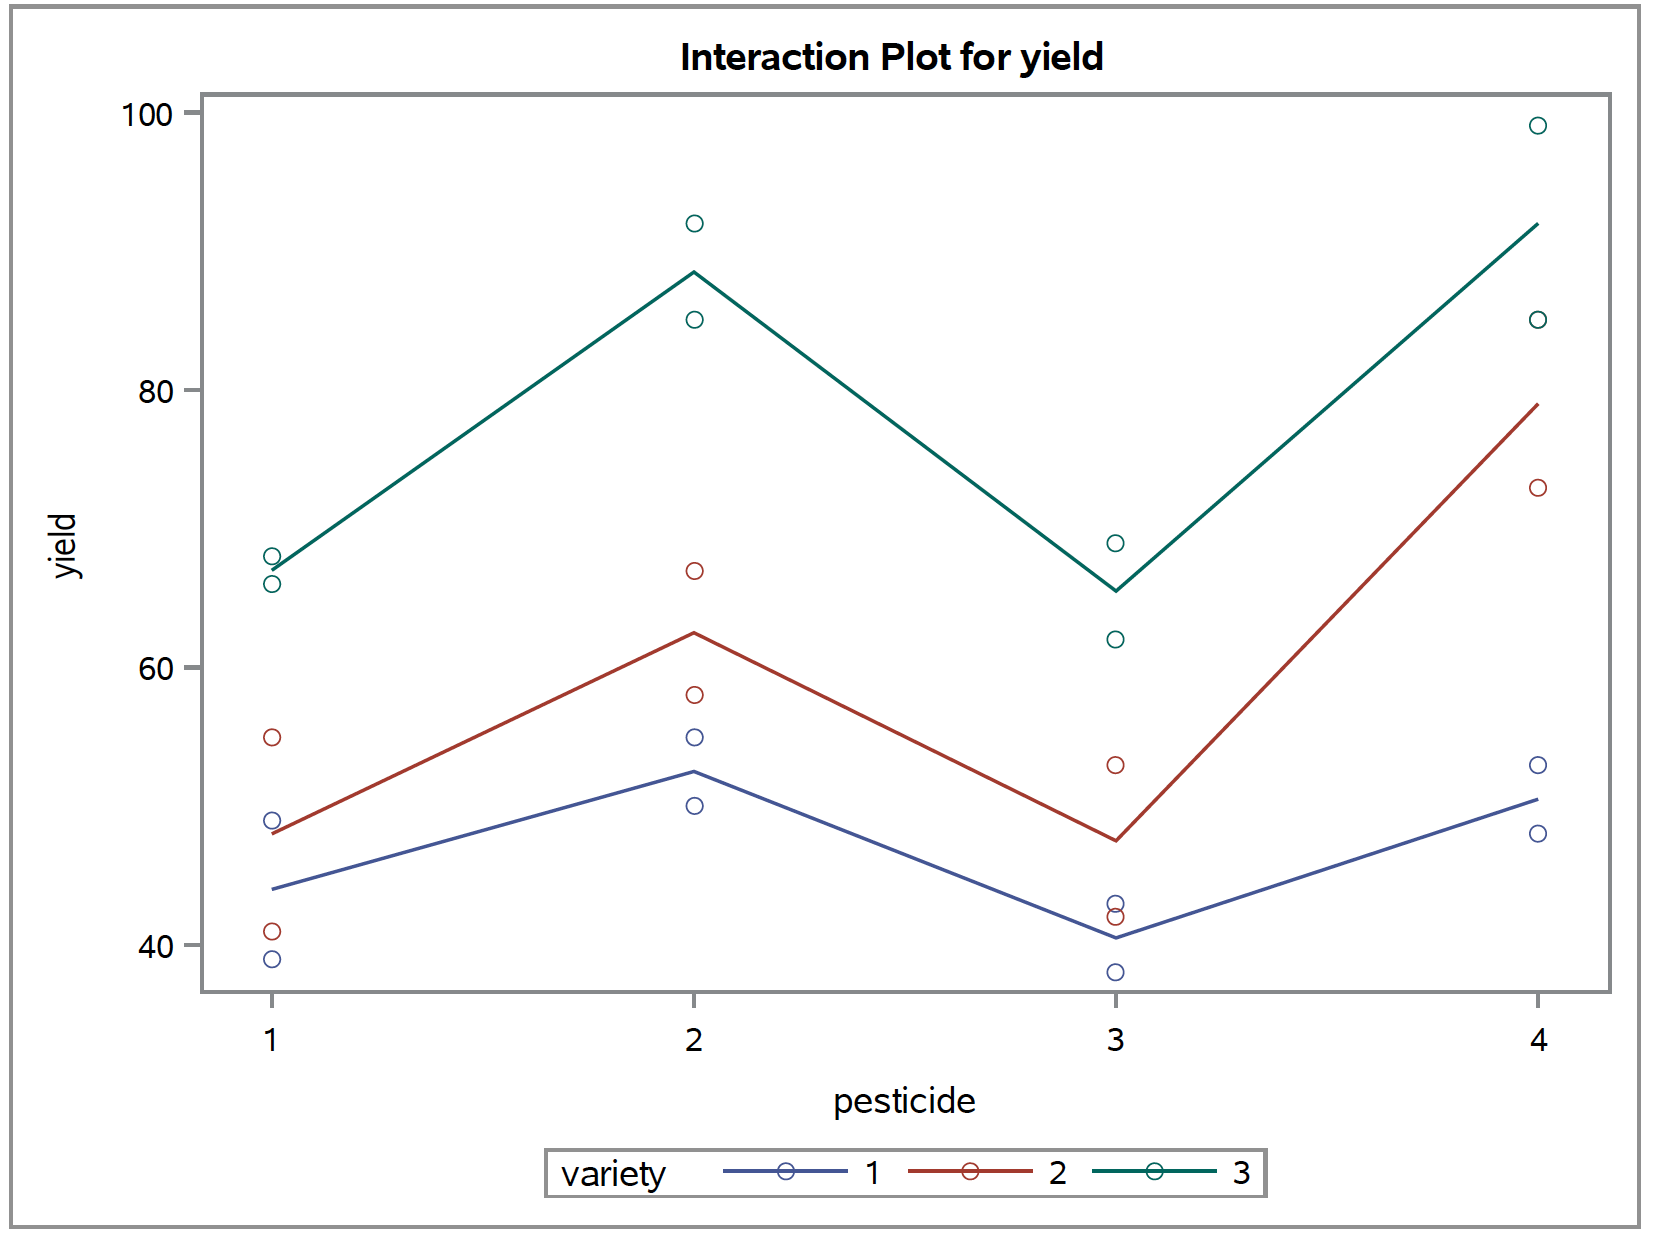
\includegraphics{factorial_interaction.png}}
\end{center}
\caption{Interaction plot for Example~14-6 in Ott \& Longnecker.}
\label{fig:factorial.interaction}
\end{figure}

To conclude this discussion about the balanced two-way factorial designs and analysis, I want to give a few technical details about the connection between orthogonal contrasts and the sums of squares for the main effects and interaction in the SAS output.  For this, let's revisit the simple $2 \times 2$ setup from before.  Define the three quantities:
\begin{align*}
\theta_A & = \tfrac12(\mu_{11} + \mu_{12}) - \tfrac12(\mu_{21} + \mu_{22}) \\
\theta_B & = \tfrac12(\mu_{11} + \mu_{21}) - \tfrac12(\mu_{12} + \mu_{22}) \\
\theta_{AB} & = \tfrac12 (\mu_{11} - \mu_{21}) - \tfrac12 (\mu_{12} - \mu_{22}).
\end{align*}
It's a simple calculation to check that (i)~these three are contrasts and (ii)~they're orthogonal; it is a mathematical fact that contrasts which are orthogonal are also linearly independent.  So these three contrasts can be pooled together into a single F test that is based on a sum of squares, $\text{SS}(\theta_A, \theta_B, \theta_{AB})$.  But since these contrasts are also orthogonal, by the theory of orthogonal contrasts described above, the $\text{SS}(\theta_A, \theta_B, \theta_{AB})$ partitions as a sum:
\[ \text{SS}(\theta_A, \theta_B, \theta_{AB}) = \text{SS}(\theta_A) + \text{SS}(\theta_B) + \text{SS}(\theta_{AB}). \]
This, on it's own, isn't particularly interesting.  The more interesting part is that the sum of squares on the left-hand side is actually a more familiar sum of squares.  In the present case, there are four total means---$\mu_{11}$, $\mu_{12}$, $\mu_{21}$, and $\mu_{22}$---so the maximal number of linearly independent contrasts is $4-1=3$.  Since here we have exactly three linearly independent contrasts, and this set is ``exhaustive'' in some sense, it follows that 
\[ \text{SS}(\theta_A, \theta_B, \theta_{AB}) = \text{SS}(\text{Model}). \]
This explains why, in the PROC GLM output, the three sums of squares---two main effects and one interaction---add up to the model sum of squares in the first ANOVA table.  In other words, these questions about the effects parameters boil down to hypotheses stated in terms of (orthogonal) contrasts.  Moreover, the test for presence of interaction can be viewed as looking at the proportion of the model sum of squares that corresponds to the interaction-focused contrast.  

\subsection*{03/26/2019}

\subsubsection*{More than two factors}

We have focused so far on one- and two-way layouts, involving one and two factors, respectively.  But if we can do two factors, then we basically know how to do three-, ten-, and 50-way layouts too.  These are conceptually the same as the two-way formulation, just more complicated to write out the details and, the more factors we have, the more homogeneous experimental units required.  

Consider a three-way setup with factors A, B, and C, whose number of levels are $a$, $b$, and $c$, respectively.  The design can be visualized as a three-dimensional array of cells, with the three dimensions corresponding to the levels of A, B, and C, respectively.  Each cell corresponds to a treatment, i.e., a combination of levels for each of the three factors, and $r$ many experimental units are assigned to each treatment.  After the experiment is finished, there are $r$ numerical entries (the response, $y$) in each cell.  This is the data we will analyze.  Of course, it's not easy to visualize a three-dimensional array so this is not how the data will be presented; it's common to draw the three-way layout via a two-way layout for each level of the third factor, and the data is usually displayed as a spreadsheet with columns for each of the factors and the response.  

Once the data is in hand, it is time to carry out the analysis, and, for the three factor case, the usual model is as follows:
\begin{align*}
y_{ijk\ell} & = \text{response at level $i$ of A, level $j$ of B, level $k$ of C, replicate $\ell$} \\
& = \mu + \alpha_i + \beta_j + \gamma_k \\
& \qquad + (\alpha\beta)_{ij} + (\alpha\gamma)_{ik} + (\beta\gamma)_{ij} \\
& \qquad + (\alpha\beta\gamma)_{ijk} \\
& \qquad + \eps_{ijk\ell}, 
\end{align*}
where $\alpha_i$, $\beta_j$, and $\gamma_k$ are the main effects for factors A, B, and C, respectively, $(\alpha\beta)_{ij}$, $(\alpha\gamma)_{ik}$, and $(\beta\gamma)_{jk}$ are the AB, AC, and BC interaction effects, respectively, $(\alpha\beta\gamma)_{ijk}$ are the ABC interaction effects, and $\eps_{ijk\ell}$ are the usual random errors, assumed to be iid $\nm(0,\sigma_\eps^2)$.  Even with only three factors, this is pretty messy---imagine with 10 factors!  

As usual, the first thing we're interested when we fit this model is if there's anything interesting going on at all.  The corresponding hypothesis is that all the means---one for each cell in the $a \times b \times c$ table---are the same or, equivalently, all the effect parameters in the above model statement are 0.  For this we can carry out the usual overall F test, the results of which are displayed in the first analysis of variance table in the SAS output.  Usually this overall F test will reject, in which case we can proceed to ask various follow-up questions.  In the two-way setup, the interesting follow-up question was about the interaction, and the same is true here.  The only difference is that there are more interaction terms.  But we start with the most complicated term, the three-way interaction, and work our way down from more to less complex.  When the design is balanced, there is a contrast corresponding to all the effects in the above model---main effects, two-way, and three-way interactions---and we can test for each of them using the output in the contrast sum of squares table in the SAS output.  For example, if we want to know if the three-way interaction is needed to explain the relationship between the variable under investigation, we consider a hypothesis 
\[ H_0: \text{all the $(\alpha\beta\gamma)_{ijk}$'s are 0}. \]
Then we find the three-way interaction row in the contrast sum of squares table and read off the corresponding F statistic and p-value.  If the p-value is small, then we conclude that the hypothesis is implausible, hence the three-way interaction is needed; otherwise we can consider to remove it, to simplify the model and move the corresponding degrees of freedom to error.  If the three-way interaction term is removed, then one can proceed to look at each of the two-way interactions in the same way.  

\begin{example}[14-7 in Ott \& Longnecker]
See SAS code on the course webpage.
\end{example}


\subsubsection*{Unbalanced designs}

In the two-way settings considered so far, we have only discussed {\em balanced designs}, where the number of replicates in each factor level combination are equal; equal replications was not important in the one-way setting.  But {\em unbalanced designs} can arise too.  For example, suppose you have two factors, A and B, each with two levels, but you only have resources for 10 experimental units.  This is not enough to do three replicates in each of the four level combinations, so you could either do an unbalanced design, e.g., 3--3--2--2, or just throw away two of the experimental units.  Often the money for the experimental units is already spent, no point in being wasteful, so one goes with an unbalanced design.  Alternatively, suppose you had enough experimental units for a balanced design but, for some reason, a plant dies or a patient moves away and the response variable can't be measured.  Then despite your best efforts to make the design balanced, it still ends up being unbalanced.  So we need to know how to handle this.  

Fortunately, very little of the analysis changes.  In fact, everything is the same except for some differences in the SAS output.  For this discussion, assume we're in a two-way setting with factors A and B.  When the design is balanced, the partition of SS(Model) into sums of squares corresponding to the main effect and interaction contrasts is unique.  However, when the design is unbalanced, it turns out there are lots of different yet interpretable ways SS(Model) can be partitioned.  Each of these different partitions corresponds to a {\em type} of sums of squares.  By default, SAS displays Type~I and Type~III; there are also Type~II, Type~IV, etc., but these are not commonly used.  When the design is balanced, these different types of sums of squares are all the same, which is why we didn't need to pay attention to which table we read our output from.  But in the unbalanced case, the sums of squares are different.  

\begin{itemize}

\item {\em Type I}. In a word, the Type~I sums of squares are {\em sequential} in the sense that they depend on the order of the factors.  That is, the sum of squares table contains the following information (and more):
\begin{center}
\begin{tabular}{cc}
\hline
Source & Type~I SS \\
\hline
A & $\text{SS}(A)$ \\
B & $\text{SS}(B \mid A)$ \\
AB & $\text{SS}(AB \mid A, B)$ \\
\hline
\end{tabular}
\end{center}
Here, $\text{SS}(A)$ is the sum of squares for factor A alone, $\text{SS}(B \mid A)$ is sum of squares for B, given A, and $\text{SS}(AB \mid A, B)$ is the sum of squares for the AB interaction, given A and B.  Notice how it is sort of building up along the ordering of the factors: first A, then add B, and then add AB interaction.  Since we generally don't have a meaningful ordering among the factors (no reason to say that A comes ``first'' before B), so the Type~I sum of squares table is {\em not} the one that we will use.  

\item {\em Type III}. In a word, the Type~III sums of squares are {\em conditional} in the sense that they look at each term given all the others.  That is, the sum of squares table contains the following information (and more):
\begin{center}
\begin{tabular}{cc}
\hline
Source & Type~III SS \\
\hline
A & $\text{SS}(A \mid B, AB)$ \\
B & $\text{SS}(B \mid A, AB)$ \\
AB & $\text{SS}(AB \mid A, B)$ \\
\hline
\end{tabular}
\end{center} 
This one treats each term---A, B, and AB---symmetrically, i.e., doesn't assume any kind of ordering.  So we will focus on the Type~III sums of squares in ST512.  

Note that the only difference between the sums of squares (and all the other output in these tables) is in the rows corresponding to main effects.  If we're investigating the importance of interaction, it doesn't matter which of the two tables we look at, since the sum of squares for AB are the same in both cases.  But care is needed when investigating main effects.  

\end{itemize}

\begin{example}[14-8 in Ott \& Longnecker]
See SAS code on the course webpage.
\end{example}





\section{Analysis of variance for blocked designs}

\subsection*{03/28/2019}

So far we've been considering cases where the available experimental units are judged to be homogeneous, or at least we don't know how they might be heterogeneous, so we rely on randomization to protect us from confounding.  But there will be cases where we know that the experimental units are not homogeneous and, more than that, we might know---or at least can measure---how and to what extent they are heterogeneous.  And in such cases, it makes sense to use that information as part of the design and analysis, so as not to put such a burden on randomization.  The way in which this information can be incorporated is through the use of {\em blocks}.  I'm going to start with a setup that is not exactly ``blocking,'' but is related and, in some sense, maybe an easier transition from the full randomization we've considered previously to the restricted randomization that's coming below.  

This first setting is commonly referred to as {\em analysis of covariance} or {\em ANCOVA} for short.  The simplest version, which is our focus here, is when there is a single factor of interest, i.e., we want to know if this one treatment affects the mean response and, if so, how.  The twist is that the experimental units might not be homogeneous, but we are able to take certain measurements that give at least some indication of heterogeneity.  As a running example, I'll consider a situation where the treatment is fertilizer and of primary interest is how it affects the mean growth of plants.  Suppose the units are small potted plants, definitely not identical.  But we might make a judgment that the development of the plants before the fertilizer treatment is started might affect how the plants respond.  To measure the pre-experimental development level, we might consider the plant heights.  So then the setup is as follows.  We take the plants and randomly allocate them to the different levels of the fertilizer treatments, but before the treatments are applied, we measure each plant's height.  Once the experiment has been carried out, we measure how much each plant has grown during the study period.  Finally, the data we have is the following 
\begin{align*}
y_{ij} & = \text{growth of the $j$th plant assigned to fertilizer type $i$} \\
x_{ij} & = \text{per-experimental height of the $j$th plant assigned to fertilizer type $i$},
\end{align*}
where $i$ indexes the fertilizer levels and $j$ indexes the replicates.  We want to make use of both the treatment levels assigned to the units and the auxiliary height measurement in our analysis of plant growth.  

For this, we can consider the following model:
\[ y_{ij} = \mu + \tau_i + \beta x_{ij} + \eps_{ij}, \]
where, as usual, the $\eps_{ij}$'s are assumed to be iid $\nm(0, \sigma_\eps^2)$.  In this model, $\mu$ is a baseline mean parameter, like an ``intercept,'' $\tau_i$ is the effect parameter corresponding to the $i$th level of the treatment, and $\beta$ is the ``slope'' parameter, all of which---in addition to the error variance, $\sigma_\eps^2$---will be estimated when we fit this model to our data using software.  We've actually seen this model before, when we discussed the incorporation of categorical predictor variables into our multiple linear regression models.  The difference is that, there, we cared mostly about how the categorical variable affected the relationship between the response and the numerical predictor, whereas here we care mostly about the treatment effects.  That is, we aren't interested in the heights of the plants before the fertilizer was applied, we simply use this height measurement in an attempt to account for the known heterogeneity.  Another ``assumption'' built in to this model specification is that the $x_{ij}$ values should not be influenced by the treatment.  The reason is that it can't be considered as a measure of the heterogeneity in the experimental units if it depends on the treatment that was applied.  This condition is not a concern if the $x_{ij}$'s are measured before the actual experiment is carried out.  For example, if I thought how the plants smelled was relevant, then I could measure that, but it would only make sense if it was before the fertilizer treatment was applied because, as I know from growing up around the cornfields of Indiana, the type of fertilizer used can affect how plants smell!

The analysis is relatively straightforward now that the model is in place.  A couple of differences here that are worth noting:
\begin{itemize}
\item The $x$ variable is numerical, not categorical, so it should not be included in the {\tt class} statement in PROC GLM.  
\item Since the $x$ variable is numerical, there is no reason to expect that there will be any kind of balance in the data set we collect.  For example, there could easily be two plants that are 6 inches tall at the start and only 1 that is 11 inches tall; the point is that we have no control over this so it's unlikely to be any kind of balance.  So when we're carrying out tests, we need to be aware that the Type~I and Type~III sum of squares tables will be different, and we should base our inferences (at least in ST512) on the Type~III table.  
\item Since we believe that the $x$ variable is important to understanding the mean response, we should incorporate that variable into the estimation of the mean response.  If we use the {\tt means} statement in PROC GLM, then we get just the average of the response variable in each of the treatment levels, which effectively ignores the $x$ variable.  But the ``least squares'' estimates of the mean response, which adjusts for $x$ by given 
\[ \hat \mu_{\text{adj}, i} = \hat\mu + \hat\tau_i + \hat\beta \bar x_{\dot\dot}, \]
where $\bar x_{\dot\dot}$ is the average value of $x$ in the data set, can be obtained by using the {\tt lsmeans} statement instead.  
\end{itemize}

\begin{example}[16-1 in Ott \& Longnecker]
See SAS code on the course webpage.
\end{example}

Next we turn to some more traditional blocking strategies.  Reconsider our original analysis of variance formulation, where we had $T$ treatment levels and a collection of (presumably homogeneous) experimental units that are randomly allocated to the treatment levels.  Now, however, suppose we {\em know} that the experimental units are not homogeneous be we know how to divide up the experimental units into groups, or {\em blocks}, consisting of roughly homogeneous units within each block, but heterogeneous between blocks.  For example, suppose we want to investigate the durability of paint used for the yellow stripes in the middle of the road.  We have $T=4$ different types of paint and, given a collection of road sections, we can randomly allocate these to a paint type, apply the paint, and measure the wear after some period of time.  However, not all roads are the same, e.g., some have higher traffic volume than others, and perhaps the traffic volume could influence the wear of the paint.  But it is possible to know which of the available sections of road are low, medium, and high traffic volumes, so we could form blocks based on the road sections' traffic volume.  And like the analysis of covariance situation described above, if we know about this heterogeneity in the experimental units, and think it might be relevant, then this should be incorporated into the analysis.  But to make this happen, we have to use the block structure carefully.  

The setup to be considered here is called a {\em randomized complete block design}, or RCBD for short.  There is a single factor or treatment of interest, with $T$ levels.  And the set of experimental units can be split into blocks which are homogeneous within blocks but heterogeneous between.  We will assume that there are $T$ many units in each of the blocks, so if there are $b$ blocks then we need $b \times T$ experimental units.\footnote{The design that has more than one unit from each block in the treatment levels is called a {\em generalized RCBD} but we will not discuss that scenario in ST512.}  The difference between RCBD and the completely randomized design described before is in how we carry out the randomization.  In the completely randomized case, the units are allocated {\em completely at random}, hence the name.  But in this RCBD, the randomization is restricted because we have to respect the block structure.  Instead, we randomly allocate one unit from every block to each treatment level.  In the end, there will be $b$ units in each treatment level, one from each block.  In the road paint example, if there are three blocks of roads---corresponding to low, medium, and high traffic---and four types of paint, then we need altogether $3 \times 4 = 12$ sections of road, four in each traffic volume block.  Then we proceed by randomly allocating the four units in a block to each of the paint types.  All of different blocking strategies in ST512 and beyond correspond to some kind of restricted randomization.  This restriction on randomization has some consequences on the analysis, which I'll explain below.  

Why do we carry out the design in this way?  An alternative strategy would be to treat the blocks like a separate factor, making it like the two-factor studies we considered previously.  There is nothing wrong with this formulation, except that it's overkill.  That is, to do the full two-way factorial study, with $r > 1$ replications, we would need $rbT$ total units.  This would give us an opportunity to fit a full two-way model and investigate interaction and main effects, but we don't actually care about all this.  Remember, the goal was to investigate just the one factor, the treatment, so we don't care about blocks or their interaction with treatment.  So the question is if it is possible save resources and use a more efficient design---with few number of units, $bT$---that allows us to answer the primary question of interest, about the treatment.  The RCBD serves this purpose.  

After properly allocating the experimental units to the treatment levels, measurements are taken and data is collected.  The data are of the form 
\[ y_{ij} = \text{response from treatment level $i$ from block $j$}. \]
To analyze these data, a commonly assumed model is 
\[ y_{ij} = \mu + \tau_i + \beta_j + \eps_{ij}, \]
where $\mu$ is a baseline level mean, $\tau_i$ is the effect for treatment level $i$, $\beta_j$ is the effect for block level $j$, and $\eps_{ij}$ are the errors assumed to be iid $\nm(0,\sigma_\eps^2)$.  Notice that, despite having two factors---treatment and block---the model {\em does not} include an interaction.  This is intentional and there are two reasons for it.  First, we do not have replications in each treatment--block combination, so we don't have sufficient data to fit such a complicated model; second, and more importantly, we are only interested in the treatment, so we don't care about interaction.  Anyway, this is just a two-way analysis of variance model but without interaction, so we can fit this using PROC GLM as usual, omitting the interaction term.  

\begin{example}[15-1 in Ott \& Longnecker]
See SAS code on the course webpage.
\end{example}

Note that {\em we do not carry out F tests concerning the block}.  For one thing, we don't care about the block so there's no reason to bother testing it; also, we already made a judgment that the block matters, otherwise we wouldn't have chosen introduce such a block in the first place.  The more subtle point is that an F test about the block is not appropriate.  The reason is that the F tests that we're familiar with are assuming that the units have been randomly allocated to the factor levels, but this is not the case for the blocks---the features that determine what block a unit is in are predetermined, not random at all.  So, besides the fact that we don't care about blocks, it is also technically not appropriate to carry out the test.  Of course, SAS doesn't know that the factor you entered in your model is block and not an actual factor, so it gives you all the output; it's up to you, the data analyst, to know what output is appropriate to use and what isn't.  There are some informal ways to assess whether the blocking factor is necessary, based on ``efficiency'' compared to analyzing the data as if it were a (gold-standard) completely randomized design.  I won't discuss this here or in lecture, but see Ott \& Longnecker, page 874, if you're interested in these details.  


\subsection*{04/02/2019}

Remember, the goal of using a carefully designed experiment was to create an opportunity in which causal conclusions could be made, e.g., the new drug {\em caused} the patients' health to improve.  And part of a good experiment was starting with a collection of {\em homogeneous} experimental units.  Randomization will probably take care of minor heterogeneity, but is not guaranteed---because it's random.  But if there is non-negligible heterogeneity, as there would be if we are even considering blocking, then it makes sense to be proactive and not rely entirely on randomization.  But how do we know that this particular type of blocking strategy is guaranteed to prevent the bias that would occur from treatment getting confounded with blocks?  To conclude this section, I'll give an answer to this question.  Unfortunately, my explanation is a bit on the technical side---lots of Greek letters---but I think it's important to demonstrate that this specific type of blocking is needed in order to eliminate potential bias from heterogeneity.  

To keep the notation as simple as possible, consider a case where the treatment has $T=2$ levels, e.g., Drug~1 and Drug~2.  Suppose we have $n=6$ experimental units, all with, say, the flu, and our goal is to learn which drug is the most effective at treating the flu.  If we believe the experimental units to be homogeneous, then we would carry use a completely randomized design (CRD) and randomly allocate, say, $r=3$ units to each of the two treatment levels, with the goal of estimating and subsequently comparing the mean responses for the two drugs.  Let $\mu_{ij}$ denote the mean response for treatment level $i$ and replication $j$; we usually don't write the second subscript, $j$, when analyzing data from a CRD because the  homogeneity assumption implies all the means in each treatment group are the same, i.e., $\mu_{i1}=\cdots=\mu_{ir}$, but this will be needed for my main point later, so please bear with me.  The replicates aren't important, so we focus on the {\em average} mean response in each treatment group:
\[ \bar\mu_{i\cdot} = \frac{\mu_{i1} + \cdots + \mu_{ir}}{r}, \quad i=1,2. \]
(For CRDs, all of these means are the same and denoted by $\mu_i$ and, of course, in such cases, $\bar \mu_{i\cdot} = \mu_i$.)  If we plug in our usual one-way model, then we have 
\begin{align*}
\bar\mu_{1\cdot} & = \mu + \tau_1 \\
\bar\mu_{2\cdot} & = \mu + \tau_2
\end{align*}
and, if we take the difference, then 
\[ \hat\mu_{1\cdot} - \hat\mu_{2\cdot} = \tau_1 - \tau_2. \]
Since the quantity on the left-hand side can be easily estimated, using the sample means in each group, so too can the right-hand side.  But the right-hand side is the difference in treatment effects, which is the quantity we care about since the goal is comparing the treatments.  This is just to set the stage, to show that the CRD allows us to make conclusions about the difference in treatments when the experimental units are homogeneous.  

Now assume that there is some heterogeneity in the experimental units.  For example, maybe two of the patients are under-average, two are average, and the other two are above-average weights; label these categories $j=1,2,3$, respectively.  If we believe that these blocks, based on weight, are relevant, then we modify the model, 
\[ \mu_{ij} = \mu + \tau_i + \beta_j, \]
to indicate that the block in which the unit comes from has an impact on the mean response.  Suppose first that we ignore this heterogeneity and carry out the CRD just like before.  When we do the random allocation, suppose we end up with 
\begin{align*}
\text{Treatment 1} & \gets \{\text{Block 1, Block 1, Block 2}\} \\
\text{Treatment 2} & \gets \{\text{Block 2, Block 3, Block 3}\}. 
\end{align*}
If we look again at the average mean response for each treatment level, but now with the inherent heterogeneity, we get 
\begin{align*}
\bar\mu_{1\cdot} & = \mu + \tau_1 + \tfrac13(\beta_1 + \beta_1 + \beta_2) \\
\bar\mu_{2\cdot} & = \mu + \tau_2 + \tfrac13(\beta_2 + \beta_3 + \beta_3). 
\end{align*}
Taking the difference we get 
\[ \bar\mu_{1\cdot} - \bar\mu_{2\cdot} = \tau_1 - \tau_2 + \{\tfrac13(\beta_1 + \beta_1 + \beta_2) - \tfrac13 (\beta_2 + \beta_3 + \beta_3)\}. \]
We can, as usual, estimate the left-hand side.  But the right-hand side no longer represents the difference in treatment effects because the block effects are also present.  The expression in braces above represents the bias resulting from unaccounted for heterogeneity in the experimental units.  How can we overcome this?  If instead of doing a complete random assignment of units to treatment levels, suppose we allocated one unit from each block to the two treatments.  That is, suppose 
\begin{align*}
\text{Treatment 1} & \gets \{\text{Block 1, Block 2, Block 3}\} \\
\text{Treatment 2} & \gets \{\text{Block 1, Block 2, Block 3}\}. 
\end{align*}
The two average mean response are 
\begin{align*}
\bar\mu_{1\cdot} & = \mu + \tau_1 + \tfrac13(\beta_1 + \beta_2 + \beta_3) \\
\bar\mu_{2\cdot} & = \mu + \tau_2 + \tfrac13(\beta_1 + \beta_2 + \beta_3) 
\end{align*}
and taking the difference we get 
\[ \bar\mu_{1\cdot} - \bar\mu_{2\cdot} = \tau_1 - \tau_2 + \{\tfrac13(\beta_1 + \beta_2+ \beta_3) - \tfrac13 (\beta_1 + \beta_2 + \beta_3)\} = \tau_1 - \tau_2. \]
That is, by forcing each treatment level to have a unit from each block, we create the kind of balance needed such that the block effects cancel, allowing us to estimate and answer subsequent questions about the difference in treatment effects.  


\subsection*{04/04/2019}

\subsubsection*{Latin square designs}

Previously we considered the case where the heterogeneity in the experimental units could be described by a single blocking factor, e.g., the traffic load for each of the road segments on which the yellow paint is to be tested.  But it could happen that two blocking factors are needed to describe the heterogeneity, in which case, a design more flexible than the RCBD is needed.  In particular, a {\em Latin square} design is for exactly this purpose.  

As a running example, consider a case where the goal is to learn about differences across brands of air filters in terms of their effectiveness.  We could identify a collection of households in which to install the air filters for a test and then randomly allocate the different brands of filters to the households.  However, there are reasons to be concerned about heterogeneity and possible confounding.  For example, we can't control what's going on in the different households so it's possible that one is ``dirtier'' than another, which can affect the air filter performance.  Also, air can be affected by time of year (e.g., North Carolina sees lots of pollen in the air during springtime) which can also affect the air filter effectiveness.  So it makes sense to consider blocking according to combinations of the levels of household and month.  

In general, if we have two blocking factors, we imagine arranging the experimental units in a grid like the one below.  The two blocking factors are generically described as Row and Column factors because of how the table is arranged, but there is nothing special about which blocking factor is called Row and which is called Column.  The version drawn below is for a $5 \times 5$ Latin square, but any other dimension square can be handled similarly.  
{\small
\begin{verbatim}
                      Column 
                 | 1  2  3  4  5
             -------------------
               1 | .  .  .  .  .
               2 | .  .  .  .  .
          Row  3 | .  .  .  .  .
               4 | .  .  .  .  .
               5 | .  .  .  .  .
\end{verbatim}
}
Note that each cell in the above grid corresponds to a single experimental unit, e.g., a particular household in a particular month.  Then the design is about how to allocate those experimental units to the levels of the treatment, in this case, the brand of air filter.  An equivalent way to think about this task, which is convenient here, is to assign the treatment levels to the different cells in the above table.\footnote{Note that we usually think about assigning experimental units to a treatment level, but there's no reason why that perspective can't be reversed; that is, to think instead about assigning treatment levels to the experimental units.}  The key point, like with the RCBD above, is that there needs to be a certain amount of {\em balance} in that allocation of treatments to experimental units, so that there is no confounding between treatment and blocks.  Again, we don't directly care about the blocking factors, only the treatment, so we're interested in the most efficient design that will allow us to answer questions about the treatment while accounting for known heterogeneity in the experimental units.  

Based on our experience with RCBD, you might anticipate how this allocation of units to the cells in the above grid might go.  That is, we want to make sure that each level of the treatment appears exactly once in every row and every column.  This requirement puts some constraints on the design setting.  In particular, it requires that the above grid be a {\em square}, i.e., that $r=c$ and that there also be the same number of treatment levels.  In our example, we have 5 households, 5 months over which the study is carried out, and 5 brands of air filter.  We typically label the treatment levels by numbers, but to see why this design is called Latin square, write the brands of air filter as A, B, C, D, and E---Latin letters.  Then the Latin square design puts these letters in the cells of the grid in such a way that each letter appears exactly once in every row and column.  One example is as follows:
{\small
\begin{verbatim}
                      Column 
                 | 1  2  3  4  5
             -------------------
               1 | A  E  D  C  B
               2 | B  A  E  D  C
          Row  3 | C  B  A  E  D
               4 | D  C  B  A  E
               5 | E  D  C  B  A
\end{verbatim}
}
This is not the only way to fill in the cells with letters; the {\em randomization} in this context is to randomly choose among the different ways to assign the letters to the grid.  If you're familiar with Sudoku puzzles you might see some similarities to the Latin square design.  In fact, the interesting structures that underly the construction of Sudoku puzzles have applications in the construction of experimental designs.

Once the treatment levels are assigned to the cells in the above grid, the experiment is carried out and data are collected.  The measurements are 
\[ y_{ijk} = \text{response in treatment $i$, row $j$, column $k$}. \]
To analyze these data, towards answering questions about the treatment, we consider the following model:
\[ y_{ijk} = \mu + \tau_i + \rho_j + \gamma_k + \eps_{ijk}, \]
where $\mu$ is a baseline mean, $\tau$ is the effect of treatment level $i$, $\rho_j$ is the effect of row\footnote{I'm using Greek letter $\rho$ (``rho'') to represent the row effect.} level $j$, $\gamma_k$ is the effect of column level $k$, and $\eps_{ijk}$ are the usual random errors, assumed to normal with mean 0 and variance $\sigma_\eps^2$ that doesn't depend on row, column, or treatment.  Two points to note:
\begin{itemize}
\item There is no interaction in this model, in part because we don't care about main effects for blocks so, likewise, we don't care about their interation with treatment or each other, but also because we don't have the replication necessary to fit a model that includes interaction.
\item Like in the RCBD context, it is not appropriate to test for significance of the row or column block effects based on this analysis.  The reason, as before, is that those F tests assume units are randomly allocated to the various levels but, in our present case, the blocks are determined by the units themselves, not randomly allocated.  Anyway, software doesn't know that a factor is a block or not, so it will report the output for these tests by default.  It's up to us to recognize which tests are appropriate to carry out and ignore the others.  
\end{itemize}

\begin{example}[15-5 in Ott \& Longnecker]
See SAS code on the course webpage.
\end{example}

There's an interesting extension of the Latin square design in which it is possible to three blocking factors with the same number of experimental units.  This is more complicated than the Latin square design so we won't cover this in any detail, but I thought it was worth at least mentioning.  The idea is to take two Latin squares having the same rows and columns, one for the treatment factor and one for the third blocking factor.  Let's look at the $5 \times 5$ case like above.  Here are two such Latin squares, where I used A, B, C, D, and E for the levels of the treatment and a, b, c, d, and e for the levels of the third blocking factor, but I should be using $\alpha$, $\beta$, $\gamma$, $\delta$, $\eps$ in the latter case,\footnote{The reason I'm not using the Greek letters here is just because I'm lazy; I'd have to write special codes to generate these tables with the regular fonts, but I can do it directly using plain text.} for reasons that will become clear shortly.  Below are two such Latin squares, though these are not the only two:
{\small
\begin{verbatim}
                    Column                            Column
               | 1  2  3  4  5                   | 1  2  3  4  5
           -------------------               ------------------
             1 | A  E  D  C  B                 1 | a  c  e  b  d
             2 | B  A  E  D  C                 2 | b  d  a  c  e
        Row  3 | C  B  A  E  D            Row  3 | c  e  b  d  a  
             4 | D  C  B  A  E                 4 | d  a  c  e  b
             5 | E  D  C  B  A                 5 | e  b  d  a  c
\end{verbatim}
}
Now superimpose the two tables, to get a new table:
{\small
\begin{verbatim}
                         Column 
                 |  1   2   3   4   5
             ------------------------
               1 | Aa  Ec  De  Cb  Bd
               2 | Bb  Ad  Ea  Dc  Ce
          Row  3 | Cc  Be  Ab  Ed  Da
               4 | Dd  Ca  Bc  Ae  Eb
               5 | Ee  Db  Cd  Ba  Ac
\end{verbatim}
}
What's special about this new table is that each of the Latin letters appears exactly once with each Greek letter (or lower-case Latin letters in my table).  Such designs are called {\em Graeco-Latin square designs}.  



\subsubsection*{Factorial-within-block designs}

Recall the situation where we had two factors of interest, call them A and B, and the treatments correspond to combinations of the levels of these two factors.  For example, suppose we are interested to understand the effect of both flour type ($a=3$ levels) and baking temperature ($b=3$ levels) on the protein content in bread.  Ideally, we could to a $3 \times 3$ factorial design with replication, say, $r=3$ replicates under each flour--temperature combination.  For such a design, we would need $3 \times 3 \times 3 = 27$ runs, but it's possible that there's not enough time to do all those runs in a single day.  If we were concerned about some differences across days, e.g., different employees making the batter or operating the ovens, then blindly extending the experiment over multiple days might introduce some bias, due to confounding factors.  

To avoid this, we want to block on days, but we don't want to increase the total number of runs.  The way these can both be achieved is by doing separate factorial experiments on the three days, where each of the $3 \times 3 = 9$ combinations of flour and temperature are run, with a single replication, on each day.  This still has 27 runs split over 3 days, but allows us to estimate flour--temperature main effects and interactions, all while controlling for possible heterogeneity across days.  

Once the experiment has been designed, the runs are carried out and the data is collected.  We get values $y_{ijk}$ corresponding to the response in level $i$ of factor A, level $j$ of factor B, in block $k$.  The model is 
\[ y_{ijk} = \mu + \alpha_i + \beta_j + (\alpha\beta)_{ij} + \gamma_k + \eps_{ijk}, \]
where $\mu$ is a baseline level mean, $\alpha_i$ and $\beta_j$ are main effects for levels $i$ and $j$ of factor A and B, respectively, $(\alpha\beta)_{ij}$ is the interaction effect, and $\gamma_k$ is the main effect for block.  As before, we do not carry out tests for the block main effect because we have not randomized over the block, in fact, block is a constraint on randomization.  Anyway, of primary interest is the interaction and main effects of the factors A and B.  We proceed with first assessing the most complicated term---the interaction---and, if this can be removed from the model, then we look at main effects and consider simplifying the model further.  

\begin{example}[15-9 in Ott \& Longnecker]
See SAS code on the course webpage.
\end{example}



\section{Random- and mixed-effects models}

\subsection*{04/09/2019}

So far, we have focused on experiments with what would be called {\em fixed-effects}.  That is, where the levels of the factors being considered were fixed in advance, prior to considerations about how the design would be laid out.  In, say, the road paint example, there were four brands of paint that were identified in advance of our considerations about how to design the experiment.  We didn't call this a fixed-effect model because, at that time, there was nothing else to compare to.  But now we're considering a different situation where the levels of the factor might be sampled at random from some population of levels.  

As an example, suppose we want to investigate some student health feature across the different high schools in North Carolina.  There are hundreds of high schools so we might not have the resources to actually go and collect data from all of them.  An idea is to take a random sample of schools from that population and collect/analyze data just from those sampled schools.  That's a perfectly reasonable idea, and analyzing the data from such an experiment isn't really any different from what we did previously, but the questions we want to answer are a bit different---of broader scope---so we have to add some assumptions, adjust how we formulate the statistical hypotheses, and in some cases be careful with how we carry out the tests.  

To set up the one-way random-effects study/model, there will be some factor/treatment of interest, with an associated population of levels.  In the running example, the factor is school and the population is all the high schools in North Carolina.  Since there's insufficient resources to look at the entire population of levels, we randomly sample $T$ many of them; in our example, let's say we have $T=10$ schools.  Experimental units are then allocated to the different factor levels and $r$ measurements of the response variable are taken on each one; e.g., maybe $r=10$ students from each sampled school are randomly sampled and they get measurements taken on their health.  This results in data $y_{ij}$, the response measured on unit $j$ in treatment level $i$.  

There will be no visible difference in the data from this experiment that will identify it as a random- instead of fixed-effect setup.  It is only through the description of how the study was carried out that random versus fixed can be determined.  The strategy is to ask the following question: {\em the experiment were repeated, would I necessarily have the same levels of the factor?}  If the answer is YES, then it's a fixed-effect study, otherwise, it's a random-effect study; there will be cases, called {\em mixed-effects} studies, where some factors are fixed and some are random, more on this later.  

Before going forward, let's review some of the basic principles of statistics you should have seen in ST511.  Remember that we don't carry out hypothesis tests, etc, {\em about the data}.  That is, I don't have to test if the {\em sample mean} is greater than 0, I just have to look at the number.  The formal test is needed because we are trying to tell if the {\em population mean} is greater than 0, but all we have is an estimate, the sample mean.  A crucial but often overlooked point is that the sample mean is informative about the population mean only if the sample is ``representative.''  Unfortunately, a judgment of ``representative'' is impossible; we'd have to know the population in question to say one way or the other.  And if we knew about the population, then we wouldn't need to do a statistical analysis in the first place.  To deal with this, we focus on the quality of the {\em procedure} by which the sample is obtained, not on the specific sample.  One way to reliably produce a ``representative'' sample is via random sampling; there are other sampling procedures that are designed to deal with constraints that prevent completely random sampling.  Anyway, if we can get a random sample from the population, then in principle we are able to make certain conclusion about the population from the obtained sample; that's what statistical inference is about.  But if we don't have a random (or otherwise ``representative'') sample, then it can be difficult to justify generalizing the conclusions from the single sample to the population.  This is why we want to avoid using so-called ``convenience samples;'' there's nothing fundamentally wrong with convenience samples, it's just that it's difficult to generalize the conclusions based on them to a bigger relevant population.  

Returning from that digression, the point is that if we get a random sample of the factor levels from the population, then it is possible to make conclusions that apply to the population, not just the factor levels we happened to sample.  So, for our example, the goal is to answer the question {\em are there any differences in the mean student health across all high schools in North Carolina?}, and this is possible through the use of these random effect studies.  The price we pay is that the randomness complicates the model to be fit; here, in ST512 and similar courses, we side-step most of this complication by adding a very special assumption, described below.\footnote{There are much more sophisticated kinds of statistical methods that, instead of making strong assumptions about the random effects distribution, try to actually estimate that distribution from the data.  In fact, some of the work that I did as part of my PhD thesis fits under this umbrella; in case you're interested, I wrote a review of this work (in honor of my PhD advisor, who recently passed away) here: \url{https://www.researchers.one/article/2018-12-5}}

When we've collected data from a one-way random-effect study, the model commonly assumed is 
\[ y_{ij} = \mu + \tau_i + \eps_{ij}, \]
where $\mu$ is a baseline level mean, $\tau_i$ is the effect of treatment level $i$, and $\eps_{ij}$ are the random errors, assumed iid $\nm(0,\sigma_\eps^2)$.  So far, this looks identical to our previous analysis of variance models.  The difference here is that the $\tau_i$'s are no longer fixed-but-unknown quantities to be estimated, they are {\em random}---because the particular level of the treatment is random.  So we have to say something about the sense in which they are random, and this is where the extra assumptions come in.  In particular, we {\em assume} that 
\[ \text{$\tau_1,\ldots,\tau_T$ are iid $\nm(0, \sigma_\tau^2)$.} \]
To be clear, this is an assumption and, unfortunately, one that is much more different to justify compared to those assumptions about the $\eps_{ij}$'s.  Now we finally see why we've been including the subscript ``$\eps$'' on the variance $\sigma_\eps^2$ all this time, because new variances are going to start showing up.  In fact, both $\sigma_\eps^2$ and $\sigma_\tau^2$ are called {\em variance components}, and we'll be seeing more of these in the coming lectures.  

Previously, in the fixed-effects setting, the way we formulated the hypothesis corresponding to the question about difference in mean response across treatment levels was 
\[ H_0: \tau_1 = \cdots = \tau_T = 0. \]
But now this hypothesis doesn't make sense because the $\tau_i$'s are not fixed numbers that we can make hypotheses about.  Moreover, this is a question just about the effects associated with the levels in this study, what we're interested in is answers questions about the population from which these effects were sampled from.  That population is characterized by the assumption about the distribution, $\nm(0, \sigma_\tau^2)$, so we should formulate our scientific question in terms of the (only) parameter in that distribution, namely, $\sigma_\tau^2$.  What would it take for all the $\tau_i$'s in the population to be equal 0?  Zero variance!  So that becomes our new hypothesis, i.e., 
\[ H_0: \sigma_\tau^2 = 0. \]
In this simple setting with only one random effect, the procedure we follow to carry out the F test is identical to what we had done before.  But there will be some differences as we get to more complicated settings.  

The adjustments we need to make to the F test will be clear from what are called the {\em expected mean squares} table that SAS reports to us when at least one effect is random.  We don't need the expected mean squares table now, but I'll explain it here anyway because we're in the simplest case; I hope this will make the discussion in the more complicated case easier.  

Recall that we used the mean square error, which I'll write here as MS(error), as an estimate of the error variance, $\sigma_\eps^2$.  The reason this is used as an estimator is because it's ``unbiased,'' i.e., 
\[ \E\{\text{MS(error)}\} = \sigma_\eps^2, \]
where $\E$ is what's called the {\em expected value} operator, and its function is to average MS(error) over all possible data sets.  But there are other mean squares and these also have expected values, in particular, 
\[ \E\{\text{MS(treatment)}\} = \sigma_\eps^2 + r \sigma_\tau^2, \]
where $r$ is the number of replications in each treatment level.  Notice that both variance components show up in this expression, and this is what allows us to isolate the variance component of interest, $\sigma_\tau^2$.  Note that, if the null hypothesis above is true, i.e., if $\sigma_\tau^2=0$, then we have 
\[ \text{MS(treatment)} \approx \text{MS(error)}. \]
Therefore, in this case, the ratio 
\[ F = \frac{\text{MS(treatment)}}{\text{MS(error)}} \]
would be close to 1.  But if $\sigma_\tau^2 > 0$, then the ratio would be bigger than 1.  This is how we isolate the treatment effect, and why we reject the null hypothesis when the F ratio is large.  When we get to the more complicated situations below, we'll apply the same logic when looking at the expected mean squares, i.e., choose the terms for the ratio that isolate the variance component of interest.  


\subsection*{04/11/2019}

Like in our previous discussion of fixed factors and analysis of variance models, there are lots of variations on the one-way random effects setup introduced above.  In particular, we can have multiple factors, all or some of which are random, with a block interpretation or as additional factors of interest in a factorial setup.  Let's talk about two such cases.  

Like in Example~17.2 in Ott \& Longnecker, consider a situation where the goal is to assess the reliability of DNA analyses across different analysts.  While the particular context to be considered here is different, such a question might be relevant in legal applications, since DNA evidence is often used but, if the DNA analysis results vary across analysts, then this could affect the reliability of DNA evidence, etc.  Anyway, here the DNA being considered is that found in plaque on subjects teeth.  There are lots of analyst with the credentials to do such an analysis, too many to study individually, so a sample of 5 analysts is taken from that population.  Similarly, there are lots of subjects available to participate in the study, so these are sampled from a large population as well.  Heterogeneity across subjects is not of scientific interest, so we treat subject as a (random) blocking factor.  The experiment is carried out as follows: 10 subjects are sampled and 5 specimens of plaque are taken from their teeth; those five specimens are then randomly allocated, one to each analyst.  So each analyst measures 10 plaque specimens, exactly one from each of the subjects.  The measurements $y_{ij}$ are summaries of the DNA measured by analyst $i$ on subject $j$.  

The model for this situation looks exactly like that for block designs with fixed effects.  That is, 
\[ y_{ij} = \mu + \tau_i + \beta_j + \eps_{ij}, \]
where $\mu$ is a baseline level mean, $\eps_{ij}$'s are random errors, $\tau_i$ is a random effect for treatment (analyst), and $\beta_j$ is a random effect for block (subject).  Each of these random effects has an associated population from which the levels are sampled, namely, 
\[ \text{$\tau_i$'s are iid $\nm(0, \sigma_\tau^2)$} \quad \text{and} \quad \text{$\beta_j$'s are iid $\nm(0, \sigma_\beta^2)$}. \]
Then $\sigma_\tau^2$, $\sigma_\beta^2$ and, of course, $\sigma_\eps^2$ are the variance components.  Note that there is no interaction between block and treatment in this model, in part because we don't care about this interaction, but also because we don't have the necessary replications to fit such a complicated model.  Since we're not interested in blocks, we proceed just like in the one-way layout considered above, and focus our attention on the variance component, $\sigma_\tau^2$, associated with the treatment (analyst).  That is, the hypothesis we wish to test is 
\[ H_0: \sigma_\tau^2 = 0, \]
and if this test rejects, then we can conclude that there are differences in the mean response across the {\em whole population} of levels of the treatment (analyst).  This test is the usual F test for main effect of treatment, since 
\[ \E\{\text{MS(treatment)}\} = \sigma_\eps^2 + b \sigma_\tau^2, \]
where $b$ is the number of block (subject) levels, $b=10$ in this case.  Note that software will give us output for testing significance of blocks, but we ignore this because it's not of interest here, and also not fully appropriate.  

\begin{example}[17-2 in Ott \& Longnecker]
See SAS code on the course webpage.
\end{example}

A second situation we'll consider here is when, as before, we have two factors of interest, say, A and B, and the treatment corresponds to combinations of the levels of these factors.  We first discussed this in the case where factors were fixed, but there's no reason we can't handle random effects in much the same way.  

Example 17-3 in Ott \& Longnecker considers a situation where interest is in measuring certain calcium levels, but it is believed that these measurements are impacted by the particular assay being used, the lab at which the measurements are taken, and perhaps on the combination of the two.  They take samples of $a=3$ assays and $b=3$ labs, and take $r=3$ calcium measurements at each of the $3 \times 3 = 9$ assay--lab combinations.  This is a factorial design, with replication, on two factors, with random levels---random because the assays and labs are sampled from a population.  The data collected consists of $y_{ijk}$ which is the calcium level measured in assay $i$, lab $j$, and replicate $k$.  A model that we might consider is 
\[ y_{ijk} = \mu + \alpha_i + \beta_j + (\alpha\beta)_{ij} + \eps_{ijk}, \]
where $\mu$ is a baseline level mean, $\alpha_i$ is the random effect corresponding to level $i$ of assay, $\beta_j$ is the random effect corresponding to level $j$ of lab, $(\alpha\beta)_{ij}$ is the random effect corresponding the the interaction of level $(i,j)$ of assay--lab, and $\eps_{ijk}$ is the error corresponding to replicate $k$ at level combination $(i,j)$.  All three of these random effects have a variance component attached to them, that is, 
\begin{align*}
\alpha_1,\ldots,\alpha_a & \iid \nm(0, \sigma_\alpha^2) \\
\beta_1, \ldots,\beta_b & \iid \nm(0, \sigma_\beta^2) \\
(\alpha\beta)_{ij} & \iid \nm(0, \sigma_{\alpha\beta}^2), \quad i=1,\ldots,a, \; j=1,\ldots,b, 
\end{align*}
where $\sigma_\alpha^2$, $\sigma_\beta^2$, and $\sigma_{\alpha\beta}^2$ are the variance components for assay, lab, and their interaction, respectively.  This model can be fit as usual in SAS, using PROC GLM, but with declaring the two factors and their interaction in the {\tt random} statement.  

In this factorial setting, there will be some differences in how the F tests are carried out.  To see this, we write out the expected mean squares for the relevant terms, namely, assay (A), lab (B), and their interaction (AB).  These take the form 
\begin{align*}
\E\{\text{MS(A)}\} & = \sigma_\eps^2 + r \sigma_{\alpha\beta}^2 + br \sigma_\alpha^2 \\
\E\{\text{MS(B)}\} & = \sigma_\eps^2 + r \sigma_{\alpha\beta}^2 + ar \sigma_\beta^2 \\
\E\{\text{MS(AB)}\} & = \sigma_\eps^2 + r \sigma_{\alpha\beta}^2 
\end{align*}
So, for tests about whether the interaction effect is significant/important, i.e., $H_0: \sigma_{\alpha\beta}^2 = 0$, the relevant F test would seek to isolate the variance component for the interaction, hence 
\[ F = \frac{\text{MS(AB)}}{\text{MS(error)}}, \]
as usual.  However, to assess the importance/significance of the main effects, for example, to test $H_0: \sigma_\alpha^2 = 0$, we need to isolate the variance component for A, hence, 
\[ F = \frac{\text{MS(A)}}{\text{MS(AB)}}. \]
That is, the F ratio this time {\em does not} have MS(error) in the denominator---this is the first time we've seen this!  This is true in general: tests about main effects in two-way ANOVA models with random effects have a modified F statistic, where interaction mean square plays the role of the error mean square.  You might notice that this situation only comes up if you are ``breaking the rules'' by testing main effects when interaction is present.  One who sticks to the policy of only testing main effects if the interaction effect is absent will not encounter this issue; even though I, personally, would adhere to this hierarchical, it's important for me to warn students about this change that arises in random effects models that include interaction.  

Another thing to be careful about is that SAS does not (without help from us) know to adjust how the F ratio is calculated in this case.  So, if you go to the line in the contrast sum of squares corresponding to the main effect, A, it will show and F statistic and p-value, {\em but this is wrong}.  That F statistic is based on MS(error) in the denominator.  To adjust for this, we have two options.  The first is to do the division, $\text{MS(A)}/\text{MS(AB)}$, ourselves; this is fine but we don't get the corresponding p-value without further efforts (with a F distribution table or R and the {\tt pf} function).  The second option is to ask SAS directly to give us output for the relevant F test.  We do this with a {\tt test} statement.  In this case, case, if we want to test $H_0: \sigma_\alpha^2 = 0$, where $\alpha$ corresponds to {\tt assay}, then we add a line 
\[ \text{\tt test h=assay e=assay*lab;} \]
This tells SAS to test the hypothesis ({\tt h}) about the assay main effect by using the mean square for the interaction {\tt assay*lab} in place of the mean square for error ({\tt e}).  This will return an extra table of output corresponding to the requested hypothesis tests.  

\begin{example}[17-3 in Ott \& Longnecker]
See SAS code on the course webpage.
\end{example}



\section{Additional topics}

Note: The material in this section will {\em not} be covered on the final exam.

\subsection*{04/23/2019}

Split-plot designs are a more general version of the kinds of factorial designs considered previously.  This generalization comes with a number of added technical complications, due to the presence of multiple variance components and nesting, but it also has a number of practical advantages, especially in agricultural and industrial applications, where it may be difficult and/or costly to vary the levels of certain key factors.  

I don't find the presentation of split-plot designs in the textbook to be especially informative, because it ultimately doesn't really explain why the model looks the way it does; none of the other books I looked at do much better.  So I'm going to try to explain things differently here, in a way that I hope makes the (admittedly weird) form of the model more understandable.\footnote{This is my first attempt at teaching this material, so this is a learning experience for me too.}  This will build on some of our recently-introduced terminology, such as random effects, variance components, etc.  

Think back to when we first discussed the completely randomized designs, with a single factor and a collection of homogeneous units.  A key element of that design was the random allocation of units to the factor levels.  As a result of that random allocation, a random effect, namely, $\eps_{ij}$, showed up in our model, having a variance component $\sigma_\eps^2$.  We didn't describe the $\eps$'s as random effects at that time, because we didn't have that terminology yet, but that's all it is.  And note that the random effect indices, the pair $(i,j)$, correspond to the experimental units, to which the randomization was applied.  The factorial designs were exactly the same, the randomization was at the experimental unit level and, therefore, the only random effect that showed up was $\eps_{ijk}$, with variance component $\sigma_\eps^2$.  In the randomized complete block designs, the situation was a little bit different, due to the restriction on randomization, but since there was no randomization associated with the blocking factor, no additional random effects turned up.  It wasn't until we discussed random effects models specifically that new random effects and variance components showed up.  A way to understand this is that the random selection of levels of the factor is an additional layer of randomization on top of that we have been applying all along.  And with this additional randomization, comes an extra random effect.  

What does this have to do with the new setup?  The split-plot design is one where, for reasons I'll describe below, the randomization is done in multiple steps and, corresponding to each randomization step, a random effect is introduced.  Consider now a situation where we have two factors, say, A and B, both of which I'll take to be fixed effects.  For example, consider a paper manufacturer who is interested in the effect of pulp preparation (A) and cooking temperature (B) on the paper strength.  Suppose there are $a=3$ pulp preparation methods and $b=4$ temperatures, and we want $r=3$ replicates.  This requires altogether $abr = 36$ runs; note that runs is the experimental unit in this case.  To carry this out as a full factorial experiment, we randomly assign runs to the preparation--temperature combinations.  So the first run could be preparation level 1 and temperature level 2, and the second run could be preparation level 3 and temperature 1, and so on.  The point is that the experimenter would likely have to change the levels at each run.  

However, it might be more convenient/economical to prepare a large batch of pulp using a single method, then split that batch into smaller portions that can be cooked at different temperatures.  For example, if one can only do 12 runs per day, then it might make sense to make a batch of pulp using each of the three preparation methods per day, divide into four portions to be cooked at different temperatures.  In that way, only nine total pulp batches need to be prepared, compared to the 36 batches required for a full factorial.  The point for doing it this way is that, presumably, it's hard to make a batch of pulp but easy to split a big batch into portions to be cooked at different temperatures, so we try to save time/money/etc by preparing as few batches of pulp as possible.  But this gain in design efficiency comes at a cost, that is, the problem formulation becomes more complicated and there is also a loss in statistical efficiency (e.g., power) behind the answers to certain questions.  

Anyway, we can imagine the design being carried out in steps as follows.  On the first day, three batches of pulp will be prepared and we randomize the order of the three preparation methods used.  Each of those batches will be split into four portions, and each portion will be randomly assigned one of the temperatures at which it will be cooked.  Using the standard terminology in this literature, the pulp preparation is called a {\em wholeplot factor} and the temperature is called a {\em subplot factor}.\footnote{Naturally, this terminology comes from agricultural applications.  In many cases, the wholeplot is a larger plot of land to which one level of a difficult-to-vary factor is applied; for example, it might be most efficient to plant a single variety of a crop over this entire plot.  Then that plot can be split into smaller regions to which different types of insecticides can easily applied.}  Obviously, this is called a {\em split-plot design} because the wholeplots are split into smaller subplots.  But what makes the model and analysis a bit more complicated in this setting is that the design is carried out in multiple steps, each of which has its own randomization element.  

The general approach has a wholeplot corresponding to factor A and a subplot corresponding to factor B, and because there's randomization that takes place at both stages, we get random effects corresponding to both wholeplot and subplot.  As before, if $y_{ijk}$ is the response (e.g., tensile strength in the paper example) at level $i$ of A, level $j$ of B, and replicate $k$, then the model takes the form 
\[ y_{ijk} = \underbrace{\mu + \alpha_i + \beta_j + (\alpha\beta)_{ij}}_{\mu_{ij}} + \text{wholeplot error} + \text{subplot error}. \]
The subplot error is effectively our familiar $\eps_{ijk}$ term, but the wholeplot error is a new object to us.  Its particular form can depend on some finer details of the design.  The situation we've been considering so far is where we have replications in the wholeplots, e.g., days in the paper example.  In that case, we are carrying out what is called a {\em completely randomized split-plot design}.  Then the wholeplot error term acts very much like the error term that showed up in our completely randomized design case; a key point here is that replicates are {\em nested} under wholeplots, e.g., the times when pulp preparation method 1 is applied corresponds to different days.  So the wholeplot error takes the form of a nested random effect
\[ \delta_{k(i)} \iid \nm(0, \sigma_\delta^2), \quad k=1,\ldots,r; \quad i=1,\ldots,a. \]
We can ask SAS to include this wholeplot error term in the model with an appropriate {\tt random} statement, including the nested factor, e.g., {\tt day(pulp)}.  Including this nested random effect will affect how the various F tests would be carried out, so it's best to see the expected mean squares table from PROC GLM or PROC MIXED.  We are interested in the factors A, B, and their interaction, so we proceed as usual with a test about the importance of the interaction term, i.e., 
\[ H_0: (\alpha\beta)_{ij} = 0 \text{ for all $(i,j)$}. \]
This is carried out via the usual F test, which takes the ratio of mean square for AB and mean square for error.  Test about the main effect for wholeplot is adjusted due to the additional wholeplot error.  The intuition behind this adjustment is that we employed a completely randomized design at the wholeplot level, so to test for the wholeplot main effect, we ought to use an F ratio that has the mean square corresponding to wholeplot error in the denominator.  

A variation on the above approach is one that treats day as a block rather than replicate.  The motivation for this alternative approach is that there may be some underlying heterogeneity due to day, in which case we'd like to control for that.  (Ott \& Longnecker, like many other books, focus almost exclusively on this blocked version of the split-plot design; I'm not sure why.)  Very little about the model formulation above changes; just like before, when we transitioned from completely randomized designs to randomized complete block designs, we add a new additive term in the model corresponding to the block.  The other change will come in the representation of the wholeplot error.  So, in the case where the replicates are treated as blocks, the model now looks like 
\[ y_{ijk} = \mu + \alpha_i + \beta_j + (\alpha\beta)_{ij} + \gamma_k + \text{wholeplot error} + \text{subplot error}, \]
where $\gamma_k$ denotes the effect for block.  (Ott \& Longnecker, like other books I found, treat $\gamma_k$ as a random effect but I wasn't able to figure out why; more on this below.)  The form of the wholeplot error will look weird, so I want to motivate it with an analogy, which requires us to reflect on some old stuff.  Recall in the case of randomized complete block designs, I said we don't include interaction between treatment and block in the model.  I gave several reasons for this, one being that there's insufficient replication to be able to estimate the interaction effect parameters.  Another way to interpret this explanation is that, without replication, {\em interaction and error are confounded}.  So, while it's not especially natural to do so, one could interpret the block--treatment interaction as a random effect and equivalent to the error in the randomized complete block design.  Take this latter interpretation and go back to the split-plot case at hand.  Now, if we're treating replicates (days) as a block, then the top level wholeplot experiment corresponds to a randomized complete block design, so now, by analogy, we can make sense of representing the wholeplot error as the block--wholeplot interaction.  Therefore, we would write the wholeplot error as a random effect of the form 
\[ (\alpha\gamma)_{ik} \iid \nm(0, \sigma_{\alpha\gamma}^2). \]
Recall my previous parenthetical point about the block being treated as a random effect; one possible explanation for this is that we're treating $\alpha$ as a fixed effect and so maybe it's weird to take $(\alpha\gamma)$ as random while both $\alpha$ and $\gamma$ are fixed.  In any case, we aren't interested in the block factor, i.e., we don't carry out tests about block, so whether it's fixed or random has no practical consequence.  As you would expect, tests about the wholeplot main effect would require some adjustment to the F ratio, but no adjustment is needed for the first quantity of interest, namely, the wholeplot--subplot interaction.  

\begin{example}[18-1 in Ott \& Longnecker]
See SAS code on the course website.
\end{example}



\subsection*{04/18/2019}

From Day~1 of the course till now, we have focused on cases where the underlying error distribution was normal.  Remember, normality is an assumption that we make, and we use the various residual plots to help justify that assumption in applications.  There are certain phenomena\footnote{The {\em central limit theorem} helps to explain why normality is common.} that suggest normality will be a reasonable assumption in many real cases, but it is by no means universal.  So a relevant question is: what to do if the normality assumption isn't justified?  In such cases, the various procedures presented in this course are not valid, so something else needs to be done.  There are basically two approaches and I'll discuss both, but I'll have more to say about the second one.  

If the procedures we discussed in the course depend on the normality assumption, can we just use some different procedures that are somehow not sensitive to departures from normality?  Such procedures are referred to as {\em robust}, {\em nonparametric}, or maybe {\em model-free}.  One example is in the context of linear regression, where the residuals obtained from the usual least-squares fit have too large of a magnitude to be normal.\footnote{Residuals with magnitude ``too large to be normal'' can be seen when, in the QQ plot, the points go way below the diagonal line on the right and/or way above the diagonal on the left.}  In such cases, we might say that there are ``outliers''---relative to a normal error model---and, since the quality of the least squares estimates deteriorates in the presence of outliers, we would consider an alternative {\em robust regression} approach.  There are lots of tools available for such a situation, but the details are beyond our scope here.  

The methods employed in ST512 were all derived based on the normality assumption.  If normality is not appropriate in a particular setting, then why not specify a different and more appropriate distribution and derive the corresponding methods?  This is an alternative approach but is much easier said than done.  Let me discuss here a specific case that is of practical relevance.  Suppose that the response variable is {\em binary}, i.e., $y$ takes only values 0 and 1.  For example, we might be interested in investigating the the relationship between some specific genetic features and the prevalence of cancer.  So the predictor variables might be a patient's gene expression levels and the response is whether or not the person has cancer.  If the response variable is binary, then a normal distribution model is definitely inappropriate; this is an extreme case, but there would be other kinds of data structure for which a normal model is not suitable.  This binary case corresponds to a different, non-normal distribution, and we can use that formulation to develop a new model and corresponding methods to describe the relationship of interest.  

Recall that, when we say a variable $y$ has a $\nm(\mu, \sigma^2)$ distribution, we are defining the probability of certain $y$ outcomes by the area under the normal bell-shaped curve.  So think of a distribution as defining probabilities, and then a model just as a device for connecting the parameters of that distribution to the relevant predictor variables.  In the binary case, there is only one relevant event, namely, $\{y=1\}$, and so the distribution is determined by the probability of that event, $\prob(y=1)$.  In the normal case, we expressed a model according to the formula 
\[ \E(y) = \beta_0 + \beta_1 x, \]
where $\E$ denotes the expected value operator; that is, we express the mean (a parameter of the normal distribution) as a linear function of the predictor variable $x$.  If we apply this same idea in the binary case, we might consider a model 
\[ \prob(y=1) = \beta_0 + \beta_1 x, \]
where we express the probability (a parameter of the binary distribution) as a linear function of the predictor variable $x$.  This, however, would not be an appropriate relationship in this case, since the probability on the left-hand side is a number between 0 and 1, while the quantity on the right-hand side can be any number.  So it is customary to make some adjustment, and the most common such adjustment is as follows:
\[ \log \Bigl\{\frac{\prob(y=1)}{1-\prob(y=1)} \Bigr\} = \beta_0 + \beta_1 x \]
or, equivalently, 
\[ \prob(y=1) = \frac{e^{\beta_0 + \beta_1 x}}{1 + e^{\beta_0 + \beta_1 x}}. \]
The model just described is called {\em logistic regression} and is widely used for analyzing data with a binary response; a plot of this logistic curve is given in Figure~\ref{fig:logistic}.  This model can be fit using what's called the {\em maximum likelihood}, which is beyond our scope here.  But this method produces estimates of $\beta$ parameters and there are corresponding hypothesis testing procedures, etc.  

\begin{example}
A widely cited example in this context is that of the 1985 Challenger space shuttle explosion.  It was eventually determined that the cause of that explosion was the failure of a particular part, called an {\em o-ring}.  Studies had been carried out to investigate the relationship between o-ring failure and launch temperature (in $^\circ$F), and the data are displayed in Figure~\ref{fig:logistic}; the values on the vertical axis are the proportion of o-ring failures in 6 experiments run at that temperature.  The pattern revealed in this plot is that o-rings seem more likely to fail when the temperature is lower.  To analyze these data more formally, and to build a model that describes this scenario, we may consider a logistic regression model.  The parameter estimates in this case are $\hat\beta_0 = 11.7$ and $\hat\beta_1=-0.22$.  That the estimated $\beta_1$ is negative implies that the failure probability is decreasing in $x$.  For visualization, the fitted logistic regression curve is overlaid on the data in Figure~\ref{fig:logistic}, and we see that this curve generally captures the shape of the data.  Like we discussed in our section on linear regression, an advantage of having such a model is that we can predict the mean response---or, in this case, the probability of o-ring failure---at any specified temperature value.  We're particularly interested in $x=32$, which was the temperature on the day of Challenger shuttle launch.  This can be seen roughly from the plot but, more precisely, the estimated probability of o-ring failure at 32 degrees is 0.99.  Unfortunately, these results were not considered on the launch day so, despite the near certainty of o-ring failure at the day's temperature based on the data analysis, they proceeded with the launch and it ended in catastrophe. 
\end{example}

\begin{figure}[t]
\begin{center}
\scalebox{0.75}{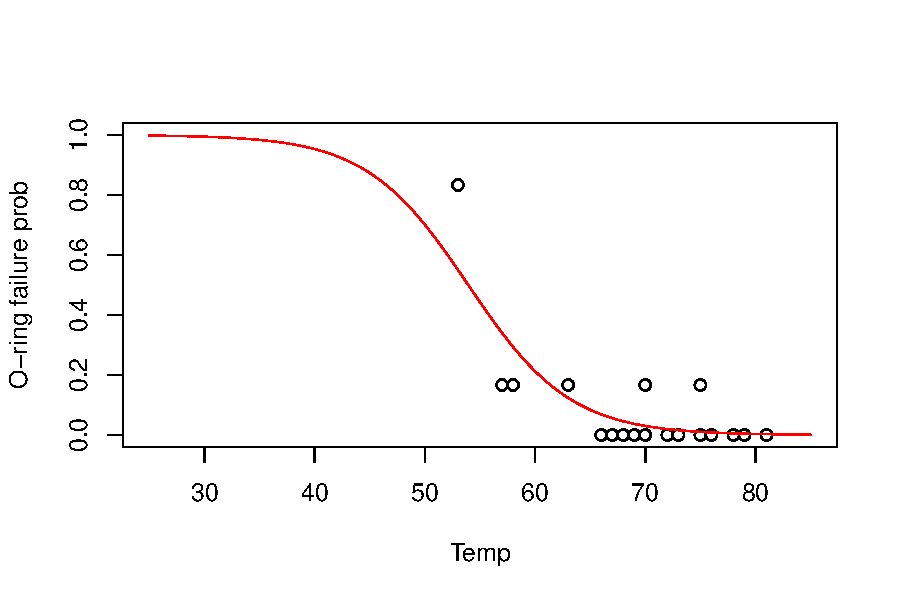
\includegraphics{oring}}
\end{center}
\caption{Plot of the o-ring failure data and the fitted logistic regression curve.}
\label{fig:logistic}
\end{figure}

\vfill

%\pagebreak


%\bibliographystyle{apalike}
%\bibliography{/Users/rgmartin/Dropbox/Research/mybib}


  




\end{document}



